% Options for packages loaded elsewhere
\PassOptionsToPackage{unicode}{hyperref}
\PassOptionsToPackage{hyphens}{url}
%
\documentclass[
  letterpaper,
  oneside,
  open=any]{scrbook}

\usepackage{amsmath,amssymb}
\usepackage{lmodern}
\usepackage{iftex}
\ifPDFTeX
  \usepackage[T1]{fontenc}
  \usepackage[utf8]{inputenc}
  \usepackage{textcomp} % provide euro and other symbols
\else % if luatex or xetex
  \usepackage{unicode-math}
  \defaultfontfeatures{Scale=MatchLowercase}
  \defaultfontfeatures[\rmfamily]{Ligatures=TeX,Scale=1}
\fi
% Use upquote if available, for straight quotes in verbatim environments
\IfFileExists{upquote.sty}{\usepackage{upquote}}{}
\IfFileExists{microtype.sty}{% use microtype if available
  \usepackage[]{microtype}
  \UseMicrotypeSet[protrusion]{basicmath} % disable protrusion for tt fonts
}{}
\makeatletter
\@ifundefined{KOMAClassName}{% if non-KOMA class
  \IfFileExists{parskip.sty}{%
    \usepackage{parskip}
  }{% else
    \setlength{\parindent}{0pt}
    \setlength{\parskip}{6pt plus 2pt minus 1pt}}
}{% if KOMA class
  \KOMAoptions{parskip=half}}
\makeatother
\usepackage{xcolor}
\setlength{\emergencystretch}{3em} % prevent overfull lines
\setcounter{secnumdepth}{5}
% Make \paragraph and \subparagraph free-standing
\ifx\paragraph\undefined\else
  \let\oldparagraph\paragraph
  \renewcommand{\paragraph}[1]{\oldparagraph{#1}\mbox{}}
\fi
\ifx\subparagraph\undefined\else
  \let\oldsubparagraph\subparagraph
  \renewcommand{\subparagraph}[1]{\oldsubparagraph{#1}\mbox{}}
\fi

\providecommand{\tightlist}{%
  \setlength{\itemsep}{0pt}\setlength{\parskip}{0pt}}\usepackage{longtable,booktabs,array}
\usepackage{calc} % for calculating minipage widths
% Correct order of tables after \paragraph or \subparagraph
\usepackage{etoolbox}
\makeatletter
\patchcmd\longtable{\par}{\if@noskipsec\mbox{}\fi\par}{}{}
\makeatother
% Allow footnotes in longtable head/foot
\IfFileExists{footnotehyper.sty}{\usepackage{footnotehyper}}{\usepackage{footnote}}
\makesavenoteenv{longtable}
\usepackage{graphicx}
\makeatletter
\def\maxwidth{\ifdim\Gin@nat@width>\linewidth\linewidth\else\Gin@nat@width\fi}
\def\maxheight{\ifdim\Gin@nat@height>\textheight\textheight\else\Gin@nat@height\fi}
\makeatother
% Scale images if necessary, so that they will not overflow the page
% margins by default, and it is still possible to overwrite the defaults
% using explicit options in \includegraphics[width, height, ...]{}
\setkeys{Gin}{width=\maxwidth,height=\maxheight,keepaspectratio}
% Set default figure placement to htbp
\makeatletter
\def\fps@figure{htbp}
\makeatother
\newlength{\cslhangindent}
\setlength{\cslhangindent}{1.5em}
\newlength{\csllabelwidth}
\setlength{\csllabelwidth}{3em}
\newlength{\cslentryspacingunit} % times entry-spacing
\setlength{\cslentryspacingunit}{\parskip}
\newenvironment{CSLReferences}[2] % #1 hanging-ident, #2 entry spacing
 {% don't indent paragraphs
  \setlength{\parindent}{0pt}
  % turn on hanging indent if param 1 is 1
  \ifodd #1
  \let\oldpar\par
  \def\par{\hangindent=\cslhangindent\oldpar}
  \fi
  % set entry spacing
  \setlength{\parskip}{#2\cslentryspacingunit}
 }%
 {}
\usepackage{calc}
\newcommand{\CSLBlock}[1]{#1\hfill\break}
\newcommand{\CSLLeftMargin}[1]{\parbox[t]{\csllabelwidth}{#1}}
\newcommand{\CSLRightInline}[1]{\parbox[t]{\linewidth - \csllabelwidth}{#1}\break}
\newcommand{\CSLIndent}[1]{\hspace{\cslhangindent}#1}

\usepackage[default]{opensans}
\fontseries{lc}\selectfont
\makeatletter
\makeatother
\makeatletter
\@ifpackageloaded{bookmark}{}{\usepackage{bookmark}}
\makeatother
\makeatletter
\@ifpackageloaded{caption}{}{\usepackage{caption}}
\AtBeginDocument{%
\ifdefined\contentsname
  \renewcommand*\contentsname{Table of contents}
\else
  \newcommand\contentsname{Table of contents}
\fi
\ifdefined\listfigurename
  \renewcommand*\listfigurename{List of Figures}
\else
  \newcommand\listfigurename{List of Figures}
\fi
\ifdefined\listtablename
  \renewcommand*\listtablename{List of Tables}
\else
  \newcommand\listtablename{List of Tables}
\fi
\ifdefined\figurename
  \renewcommand*\figurename{Figure}
\else
  \newcommand\figurename{Figure}
\fi
\ifdefined\tablename
  \renewcommand*\tablename{Table}
\else
  \newcommand\tablename{Table}
\fi
}
\@ifpackageloaded{float}{}{\usepackage{float}}
\floatstyle{ruled}
\@ifundefined{c@chapter}{\newfloat{codelisting}{h}{lop}}{\newfloat{codelisting}{h}{lop}[chapter]}
\floatname{codelisting}{Listing}
\newcommand*\listoflistings{\listof{codelisting}{List of Listings}}
\makeatother
\makeatletter
\@ifpackageloaded{caption}{}{\usepackage{caption}}
\@ifpackageloaded{subcaption}{}{\usepackage{subcaption}}
\makeatother
\makeatletter
\@ifpackageloaded{tcolorbox}{}{\usepackage[many]{tcolorbox}}
\makeatother
\makeatletter
\@ifundefined{shadecolor}{\definecolor{shadecolor}{rgb}{.97, .97, .97}}
\makeatother
\makeatletter
\makeatother

\usepackage{hyphenat}
\usepackage{ifthen}
\usepackage{calc}
\usepackage{calculator}

\usepackage{graphicx}
\usepackage{wallpaper}

\usepackage{geometry}

\usepackage{graphicx}
\usepackage{geometry}
\usepackage{afterpage}
\usepackage{tikz}
\usetikzlibrary{calc}
\usetikzlibrary{fadings}
\usepackage[pagecolor=none]{pagecolor}



% Set the titlepage font families







% Set the coverpage font families





\ifLuaTeX
  \usepackage{selnolig}  % disable illegal ligatures
\fi
\IfFileExists{bookmark.sty}{\usepackage{bookmark}}{\usepackage{hyperref}}
\IfFileExists{xurl.sty}{\usepackage{xurl}}{} % add URL line breaks if available
\urlstyle{same} % disable monospaced font for URLs
\hypersetup{
  pdftitle={NW Viability Report 2020},
  pdfauthor={Mike Ford},
  hidelinks,
  pdfcreator={LaTeX via pandoc}}

\title{NW Viability Report 2020}
\author{Mike Ford}
\date{}

\begin{document}
%%%%% begin titlepage extension code

  \begin{frontmatter}

\begin{titlepage}
% This is a combination of Pandoc templating and LaTeX
% Pandoc templating https://pandoc.org/MANUAL.html#templates
% See the README for help

\thispagestyle{empty}

\newgeometry{top=-100in}

% Page color

\newcommand{\coverauthorstyle}[1]{{\fontsize{20}{24.0}\selectfont
#1}}

\begin{tikzpicture}[remember picture, overlay, inner sep=0pt, outer sep=0pt]

\tikzfading[name=fadeout, inner color=transparent!0,outer color=transparent!100]
\tikzfading[name=fadein, inner color=transparent!100,outer color=transparent!0]
\node[anchor=south west, rotate=0.0, opacity=1.0] at ($(current page.south west)+(0pt, 8.75in)$) {

\includegraphics[width=\paperwidth, keepaspectratio]{images/cover-header-2.png}};

% Title
\newcommand{\titlelocationleft}{2.3in}
\newcommand{\titlelocationbottom}{7in}
\newcommand{\titlealign}{left}

\begin{scope}
{%
\fontsize{30}{36.0}\selectfont
\node[anchor=north
west, align=left, rotate=0] (Title1) at ($(current page.south west)+(\titlelocationleft,\titlelocationbottom)$)  [text width = 5in]  {\textcolor{black}{\bfseries{\nohyphens{NW
Viability Report 2020}}}};
}
\end{scope}

% Author
\newcommand{\authorlocationleft}{2.3in}
\newcommand{\authorlocationbottom}{5in}
\newcommand{\authoralign}{left}

\begin{scope}
{%
\fontsize{20}{24.0}\selectfont
\node[anchor=north
west, align=left, rotate=0] (Author1) at ($(current page.south west)+(\authorlocationleft,\authorlocationbottom)$)  [text width = 5in]  {
\coverauthorstyle{Mike Ford\\}};
}
\end{scope}

% Header
\newcommand{\headerlocationleft}{2.3in}
\newcommand{\headerlocationbottom}{9.8in}
\newcommand{\headerlocationalign}{left}

\begin{scope}
{%
\fontsize{16}{19.2}\selectfont
 \node[anchor=north west, align=left, rotate=0] (Header1) at %
($(current page.south west)+(\headerlocationleft,\headerlocationbottom)$)  [text width = 5in]  {\textcolor{white}{\nohyphens{NOAA
Technical Memorandum NMFS-XXX-\#\#}}};
}
\end{scope}

% Footer
\newcommand{\footerlocationleft}{6in}
\newcommand{\footerlocationbottom}{0.1\paperheight}
\newcommand{\footerlocationalign}{left}

\begin{scope}
{%
\fontsize{8}{9.6}\selectfont
 \node[anchor=north west, align=left, rotate=0] (Footer1) at %
($(current page.south west)+(\footerlocationleft,\footerlocationbottom)$)  [text width = 2.5in]  {{\nohyphens{U.S.
DEPARTMENT OF COMMERCE\\
\strut \\
National Oceanic and Atmospheric Administration\\
National Marine Fisheries Service\\
Northwest Fisheries Science Center}}};
}
\end{scope}

\end{tikzpicture}
\clearpage
\restoregeometry
%%% TITLE PAGE START

% Set up alignment commands
%Page
\newcommand{\titlepagepagealign}{
\ifthenelse{\equal{left}{right}}{\raggedleft}{}
\ifthenelse{\equal{left}{center}}{\centering}{}
\ifthenelse{\equal{left}{left}}{\raggedright}{}
}
%% Titles
\newcommand{\titlepagetitlealign}{
\ifthenelse{\equal{left}{right}}{\raggedleft}{}
\ifthenelse{\equal{left}{center}}{\centering}{}
\ifthenelse{\equal{left}{left}}{\raggedright}{}
\ifthenelse{\equal{left}{spread}}{\makebox[\linewidth][s]}{}
}


\newcommand{\titleandsubtitle}{
% Title and subtitle
{\fontsize{30}{36.0}\selectfont
\textcolor{black}{\bfseries{\nohyphens{NW Viability Report 2020}}}\par
}%
}
\newcommand{\titlepagetitleblock}{
\titleandsubtitle
}

\newcommand{\authorstyle}[1]{{\fontsize{20}{24.0}\selectfont
#1}}

\newcommand{\affiliationstyle}[1]{{#1}}

\newcommand{\titlepageauthorblock}{
\authorstyle{%
Mike Ford{\textsuperscript{1}}
}}

\newcommand{\titlepageaffiliationblock}{
\hangindent=1em
\hangafter=1
\affiliationstyle{
{1}.~NOAA Fisheres, Northwest Fisheries Science Center


\vspace{1\baselineskip} 
}
}
\newcommand{\headerstyled}{%
{}
}
\newcommand{\footerstyled}{%
{}
}
\newcommand{\datestyled}{%
{}
}


\newcommand{\titlepageheaderblock}{\headerstyled}

\newcommand{\titlepagefooterblock}{
\footerstyled
}

\newcommand{\titlepagedateblock}{
\datestyled
}

%set up blocks so user can specify order
\newcommand{\titleblock}{{\titlepagetitlealign

{\titlepagetitleblock}
}

\vspace{4\baselineskip}
}

\newcommand{\authorblock}{{\titlepageauthorblock}

\vspace{2\baselineskip}
}

\newcommand{\affiliationblock}{{\titlepageaffiliationblock}

\vspace{2\baselineskip}
}

\newcommand{\logoblock}{}

\newcommand{\footerblock}{}

\newcommand{\dateblock}{}

\newcommand{\headerblock}{}
\newgeometry{top=3in,bottom=1in,right=1in,left=1.75in}
% background image
\newlength{\bgimagesize}
\setlength{\bgimagesize}{0.75\paperwidth}
\LENGTHDIVIDE{\bgimagesize}{\paperwidth}{\theRatio} % from calculator pkg
\ThisULCornerWallPaper{\theRatio}{images/corner-image.png}

\thispagestyle{empty} % no page numbers on titlepages


\newcommand{\vrulecode}{\rule{\vrulewidth}{\textheight}}
\newlength{\vrulewidth}
\setlength{\vrulewidth}{0pt}
\newlength{\B}
\setlength{\B}{\ifdim\vrulewidth > 0pt 0.05\textwidth\else 0pt\fi}
\newlength{\minipagewidth}
\ifthenelse{\equal{left}{left} \OR \equal{left}{right} }
{% True case
\setlength{\minipagewidth}{\textwidth - \vrulewidth - \B - 0.1\textwidth}
}{
\setlength{\minipagewidth}{\textwidth - 2\vrulewidth - 2\B - 0.1\textwidth}
}
\ifthenelse{\equal{left}{left} \OR \equal{left}{leftright}}
{% True case
\raggedleft % needed for the minipage to work
\vrulecode
\hspace{\B}
}{%
\raggedright % else it is right only and width is not 0
}
% [position of box][box height][inner position]{width}
% [s] means stretch out vertically; assuming there is a vfill
\begin{minipage}[b][\textheight][s]{\minipagewidth}
\titlepagepagealign
\headerblock

\titleblock

\authorblock

\affiliationblock

\vfill

\logoblock

\footerblock
\par

\end{minipage}\ifthenelse{\equal{left}{right} \OR \equal{left}{leftright} }{
\hspace{\B}
\vrulecode}{}
\clearpage
\restoregeometry
%%% TITLE PAGE END
\end{titlepage}
\setcounter{page}{1}
\end{frontmatter}

%%%%% end titlepage extension code\ifdefined\Shaded\renewenvironment{Shaded}{\begin{tcolorbox}[enhanced, sharp corners, interior hidden, borderline west={3pt}{0pt}{shadecolor}, breakable, frame hidden, boxrule=0pt]}{\end{tcolorbox}}\fi

\renewcommand*\contentsname{Table of contents}
{
\setcounter{tocdepth}{1}
\tableofcontents
}
\listoffigures
\listoftables
\mainmatter
\bookmarksetup{startatroot}

\hypertarget{preface}{%
\chapter*{Preface}\label{preface}}
\addcontentsline{toc}{chapter}{Preface}

\markboth{Preface}{Preface}

This report can be cited as:

Northwest Fisheries Science Center. 2021. Biological viability
assessment update for Pacific salmon and steelhead listed under the
Endangered Species Act: Pacific Northwest.

Author contributions:

\begin{itemize}
\tightlist
\item
  Christopher Jordan: Interior Columbia
\item
  Damon Holzer: maps
\item
  Elizabeth Eli Holmes: status and trends analyses and graphs
\item
  James Myers: Lower Columbia, Willamette, Puget Sound
\item
  Katie Barnas: data management, habitat
\item
  Laurie Weitkamp: Oregon coast
\item
  Lisa Crozier: climate, environment
\item
  Mari Williams: Interior Columbia
\item
  Martin Liermann: Lake Ozette
\item
  Michael Ford: editor, project management
\item
  Mindy Rowse: Puget Sound
\item
  Monica Diaz: data management
\end{itemize}

\bookmarksetup{startatroot}

\hypertarget{introduction-and-summary-of-conclusions}{%
\chapter{Introduction and summary of
conclusions}\label{introduction-and-summary-of-conclusions}}

In the Pacific Northwest, there are currently 17 distinct population
segments (DPS) or evolutionarily significant units (ESUs){[}\^{}2{]} of
Pacific salmon and steelhead listed as threatened or endangered under
the Endangered Species Act (ESA) (Table 1). The ESA requires that the
National Marine Fisheries Service (NMFS) review the status of listed
species under its authority at least every five years and determine
whether any species should be removed from the list or have its listing
status changed. The most recent such review for ESA listed salmon in the
Pacific Northwest occurred in 2016
(https://www.fisheries.noaa.gov/action/2016-5-year-reviews-28-listed-species-pacific-salmon-steelhead-and-eulachon).
NMFS is again conducting such a review in 2020/21 (84 FR 53117).

The NMFS West Coast Region is responsible for the 5-year review process
for Pacific salmon and steelhead and for decision-making regarding any
proposed changes in listing status. This report provides updated
information and analyses on the biological viability of the listed
species, focusing primarily on trends and status in abundance,
productivity, spatial structure and diversity. In some cases, the report
considers new information available on ESU or population boundaries.
Where possible, this review also summarizes current information with
respect to recovery goals identified in recovery plans or Technical
Recovery Team viability documents.

In three prior viability reports that supported the current listings
NWFSC (2015) the report categorized each ESU as either ``in danger of
extinction'', ``likely to become endangered'' or ``not likely to become
endangered'', based on the ESU's abundance, productivity, spatial
structure and diversity. In a fourth report (Oregon Coast coho salmon;
Stout et al. (2012) ), the three categories were instead referred to as
``high'', ``moderate'' and ``low'' risk, and included narrative
definitions for the ``high'' and ``moderate'' risk categories (see
p.~114 of Stout \emph{et al}. 2012). In this report we use the ``high'',
``moderate'', ``low'' risk categories of Stout et al. (2012). In
addition, we also note whether the viability of each ESU appears to be
unchanged, improving, or declining, even if the magnitude of the change
is not sufficient to warrant a move among the three risk categories
(Table 1). The information in the report will be incorporated into the
Region's review, and the Region will make final determinations about
whether changes in listing status are or are not warranted, taking into
account not only biological information but also ongoing or planned
protective efforts and recovery actions.

Several ESU/DPS were evaluated to have a declining trend in overall
status since the last review (Table 1). Upper Willamette steelhead and
Chinook salmon were judged to have declining viability due to
chronically declining abundance and persistent concerns regarding
spatial structure and diversity. Snake River sockeye was judged to have
a declining viability trend, the result of abundance declines combined
with very high vulnerability to climate change. In contrast, a few
ESU/DPS were evaluated to be improving in viability. Lower Columbia
Chinook salmon were judged to have an increasing viability trend, the
result of natural spawner increases in multiple populations combined
with dramatic improvements in the fraction natural origin spawners in
several populations. Columbia River chum also showed marked improvement
in abundance for several extant populations, although many historical
populations remain extirpated or at extremely low abundance. Puget Sound
steelhead also showed some evidence of improving viability, with the
reversal of some previous strong negative trends.

Table -- Summary of current ESA listing status, recent trends and
summary of conclusions

\begin{longtable}[]{@{}
  >{\raggedright\arraybackslash}p{(\columnwidth - 8\tabcolsep) * \real{0.2000}}
  >{\raggedright\arraybackslash}p{(\columnwidth - 8\tabcolsep) * \real{0.2000}}
  >{\raggedright\arraybackslash}p{(\columnwidth - 8\tabcolsep) * \real{0.2000}}
  >{\raggedright\arraybackslash}p{(\columnwidth - 8\tabcolsep) * \real{0.2000}}
  >{\raggedright\arraybackslash}p{(\columnwidth - 8\tabcolsep) * \real{0.2000}}@{}}
\caption{Table . 15-year trends in log natural spawner abundance
computed from a linear regression applied to the smoothed natural
spawner log abundance estimate. Only populations with at least 4 natural
spawner estimates from 1980 to 2014 are shown and with at least 2 data
points in the first 5 years and last 5 years of the 15-year
period.}\tabularnewline
\toprule()
\endhead
\textbf{Species} & \textbf{ESU/DPS} & \textbf{ESA listing status} &
\textbf{Recent viability trend\textsuperscript{1}} & \textbf{2020
extinction risk category\textsuperscript{2}} \\
Chinook & Upper Columbia spring & Endangered & unchanged & high \\
& Snake River spring/summer & Threatened & unchanged &
moderate-to-high \\
& Snake River fall & Threatened & unchanged & moderate-to-low \\
& Upper Willamette & Threatened & declining & moderate \\
& Lower Columbia & Threatened & increasing & moderate \\
& Puget Sound & Threatened & unchanged & moderate \\
Coho & Lower Columbia & Threatened & unchanged & moderate \\
& Oregon Coast & Threatened & unchanged & moderate-to-low \\
Sockeye & Snake River & Endangered & declining & high \\
& Lake Ozette & Threatened & mixed & moderate-to-high \\
Chum & Hood Canal summer & Threatened & unchanged & moderate-to-low \\
& Columbia River & Threatened & unchanged & moderate \\
Steelhead & Upper Columbia & Threatened & unchanged & high \\
& Snake River & Threatened & unchanged & moderate \\
& Middle Columbia & Threatened & unchanged & moderate \\
& Upper Willamette & Threatened & declining & moderate-to-high \\
& Lower Columbia & Threatened & unchanged & moderate \\
& Puget Sound & Threatened & increasing & moderate \\
\bottomrule()
\end{longtable}

\textsuperscript{1}Recent viability trend summarizes the short-term
trend in viability for each ESU/DPS since the prior status review, based
on the expert opinion of the chapter author considering all four VSP
criteria (abundance, productivity, spatial structure and diversity).

\textsuperscript{2} High risk: A DPS or ESU with a high risk of
extinction is at or near a level of abundance, productivity, spatial
structure or diversity that places its persistence in question, such
that the risk of extinction is more than 5\% in 100 years. The
demographics of a species/DPS at such a high level of risk may be highly
uncertain and strongly influenced by stochastic or depensatory
processes. Similarly, a species/DPS may be at high risk of extinction if
it faces clear and present threats (e.g., confinement to a small
geographic area, imminent destruction, modification or curtailment of
its habitat, or disease epidemic) that are likely to create such
imminent demographic risk. Moderate risk: A DPS or ESU is at moderate
risk of extinction if it exhibits a trajectory indicating that it is
more likely than not to be at a high level of extinction risk within
30-80 years. A DPS/ESU may be at moderate risk of extinction due to
projected threats or declining trends in abundance, productivity,
spatial structure, or diversity. Low risk: neither moderate nor high
risk.

\bookmarksetup{startatroot}

\hypertarget{methods}{%
\chapter{Methods}\label{methods}}

This report includes both a set of common analyses conducted for each
ESU as well as in some cases ESU-specific analyses developed by the
individual technical recovery teams (TRTs). Here, we describe only the
common set of analyses; see the individual sections for a description of
the analyses that pertain to specific ESUs. Abundance and productivity
were generally analyzed using quantitative methods, while spatial
structure and diversity were analyzed qualitatively.

All of the Pacific Northwest TRTs spent considerable time and effort
developing spawning abundance data for the populations they identified
within ESUs. In almost all cases these estimates are derived from state,
tribal or federal monitoring programs. The raw information upon which
the spawning abundance estimates were developed consists of numerous
types of data, including redd counts, dam counts, carcass surveys,
information on pre-spawning mortality, and distribution within
populations, which the TRTs used to develop estimates of natural origin
spawning abundance. It is important to recognize that spawning abundance
estimates and related information such as the fraction of spawners that
are natural origin are not in most cases `facts' that are known with
certainty. Rather, they typically are estimates based on a variety of
sources of information, some known with greater precision or accuracy
than others. Ideally, these estimates would be characterized by a good
understanding of the degree of variation due to measurement error.
However, for the most part such a statistical characterization is either
not possible or has not been attempted, although many improvements have
been made in the last decade (see specific chapters for details). The
spawning time series summarized here and references to the methods and
sources for their development are available from the Northwest Fisheries
Science Center's Salmon Population Summary database and are also
discussed in the ESU-specific chapters.

\hypertarget{common-metrics}{%
\section{Common metrics}\label{common-metrics}}

Multivariate dynamic linear modeling (DLM) was used to estimate
population-specific mean trends in each ESU from the log of total
spawner counts. The result is an estimate of the mean or smoothed total
spawner counts, from which summary statistics regarding trends were
computed. We focus exclusively on fish spawning in nature, but often
these naturally spawning populations include some numbers of
hatchery-origin fish, either as part of a deliberate supplementation
effort or due to straying from hatchery programs. For the rest of this
report, a ``natural-origin'' or ``wild'' fish refers to a fish whose
parents spawned naturally, and a ``hatchery-origin'' fish refers to a
fish whose parents were spawned in a hatchery, regardless of prior
generation origin.

In order to estimate the trend of natural-origin spawners in populations
that also include hatchery-origin spawners, a univariate DLM was applied
to the logit of the fraction natural-origin estimate to produce a
smoothed proportion natural-origin time series. This was used to produce
an estimate of the mean natural-origin spawners for years when fraction
natural-origin estimates were unavailable.

The mean or smoothed total spawner count is similar in concept to a 3-
or 5-year geometric mean; the goal is the same---to produce an estimate
that smooths over single year variation. Such variation arises from
observation error in the spawning counts and also from peaks and troughs
in spawners numbers due to the life-history of salmonids or
environmental variation. The multivariate DLM approach has a number of
advantages. Most importantly it is a statistical model for which
maximum-likelihood diagnostics, model selection criteria, and confidence
intervals are available. It is a time-series model, which addresses
temporal autocorrelation in the data. Where there are missing data, it
provides an estimate for the missing year with appropriately wider
confidence intervals. And lastly, it allows us to use information across
all populations within an ESU to estimate the level of year-to-year
variation in the mean spawner count---the process variance---and allows
us to estimate the year-to-year covariance, which is often high, across
populations within an ESU. The latter improves estimation of missing
values because populations with data in one year help inform the values
for populations with missing data that year.

\hypertarget{dynamic-linear-modeling-for-time-varying-trend-estimation}{%
\section{Dynamic linear modeling for time-varying trend
estimation}\label{dynamic-linear-modeling-for-time-varying-trend-estimation}}

Dynamic linear models (DLMs) are similar to linear regression models
with a yearly trend. Like a classic trend analysis using linear
regression, the goal is to estimate the mean spawner count at \emph{x},
where \emph{x} is year (time). Linear regression models, however, use a
time-constant yearly trend (which appears as the regression line versus
time) while DLMs allow the trend to be time-varying.

In mathematical terms this means that the classic linear regression of
log spawners (\emph{y}) against year treats the trend (β) or yearly
growth in the mean spawner count as a constant and fits the following
model:

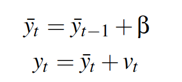
\includegraphics[width=0.61in,height=\textheight]{content/../media/image1.png}

where \emph{y\textsubscript{t}}are the observations, yt is the mean of
\emph{y\textsubscript{t}} and \emph{v\textsubscript{t}} are
normal-distributed errors. The mean spawner count in year \emph{t} is
the mean spawner count in year \emph{t−} 1 plus the constant trend value
β. Normally, we write this model in classic linear regression form as

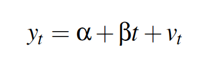
\includegraphics[width=0.69in,height=\textheight]{content/../media/image2.png}

with the mean of \emph{y\textsubscript{t}} equal to α + β\emph{t}. A
DLM, in contrast, allows us to fit a model with a time-varying β.
Specifically, the following model

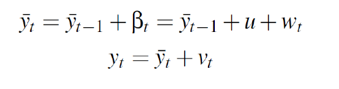
\includegraphics[width=1.13in,height=\textheight]{content/../media/image3.png}

The time-varying β is modeled as \emph{u} + \emph{w\textsubscript{t}},
where \emph{w\textsubscript{t}} is a normally distributed random
variable.

Figure 1 shows example spawner data where a time-varying sinusoidal β
(yearly growth rate) was used to generate counts (the circles) using the
DLM model above. The black line in the top panel of Figure 1 shows the
true mean \emph{y}. The red line shows the estimate from a linear
regression of \emph{y} against year with a non-time-varying β. The blue
line shows the estimate from a DLM where the β is allowed to vary in
time. The bottom panel shows the estimate of β compared to the true
sinusoidal β that generated the data. This illustrates the power of DLM
when the objective is to estimate a time-varying trend.

\hypertarget{multivariate-dlms-for-analysis-of-multiple-time-series-from-one-esu}{%
\section{Multivariate DLMs for analysis of multiple time series from one
ESU}\label{multivariate-dlms-for-analysis-of-multiple-time-series-from-one-esu}}

A multivariate DLM allows one to estimate time-varying trends using a
multiple observed time series, in our case populations within ESU, where
parameter sharing is allowed across the time series. Specifically, one
can constrain the variances to be the same across time series and to
allow covariance across time series. The latter allows information from
time series with data in year \emph{t} to help inform the estimate of
mean \emph{y} for time series that have no data in year \emph{t}. The
multivariate DLM allowed us to use all spawner count information in the
ESU to deal with measurement error in the spawner count data and more
importantly to estimate missing spawner count data.

Mathematically, the model being fit is

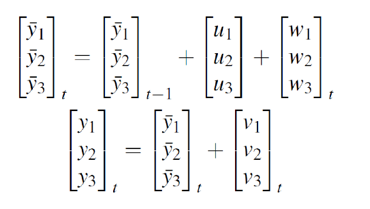
\includegraphics[width=1.23in,height=\textheight]{content/../media/image4.png}

The \emph{u\textsubscript{j}} are the long-term mean of
β\emph{\textsubscript{j,t}} . The trend at year \emph{t} is
β\emph{\textsubscript{j,t}} = \emph{u\textsubscript{j}} +
\emph{w\textsubscript{j,t}} . The \emph{w\textsubscript{t}} and
\emph{v\textsubscript{t} } are error terms drawn from a multivariate
normal distribution with variance-covariance matrix \textbf{Q} and
\textbf{R} respectively. The structure of \textbf{Q} and \textbf{R}
allows one to specify different types of parameter constraints (for
example equal variances across populations).

\hypertarget{model-selection}{%
\section{Model selection}\label{model-selection}}

Model selection was used to select the structure of \textbf{Q} and
\textbf{R}. The following structures were explored for \textbf{Q}:
diagonal with unequal variances (no covariance across populations in
terms of good and bad years and populations allowed to have different
year-to-year variability), diagonal with equal variances (no covariance
across populations and populations constrained to have the same
year-to-year variability), one variance and one covariance across all
populations, equal variances and covariances across similar run timings
in a population, and unconstrained (unique variances and covariances
across all populations). For \textbf{R} the following structures were
explored: diagonal with unequal variances (no covariance) and diagonal
with equal variances. The \textbf{R} represents the residual
non-time-dependent error and was assumed not to covary across
populations (\textbf{Q} and \textbf{R} cannot both have covariance terms
in the DLM due to identifiability constraints). Across the majority of
ESUs, model selection gave the most data support (quantified with AICc)
to a \textbf{Q} with one variance and one covariance across all
populations in an ESU and an \textbf{R}, the residual
variance-covariance matrix, with one variance across populations.
Because \textbf{Q} has covariance terms, estimates of mean spawner
numbers can be provided for populations with missing data because the
data from other populations helps inform the estimates (Figure 2 shows
an example).

\begin{figure}

{\centering 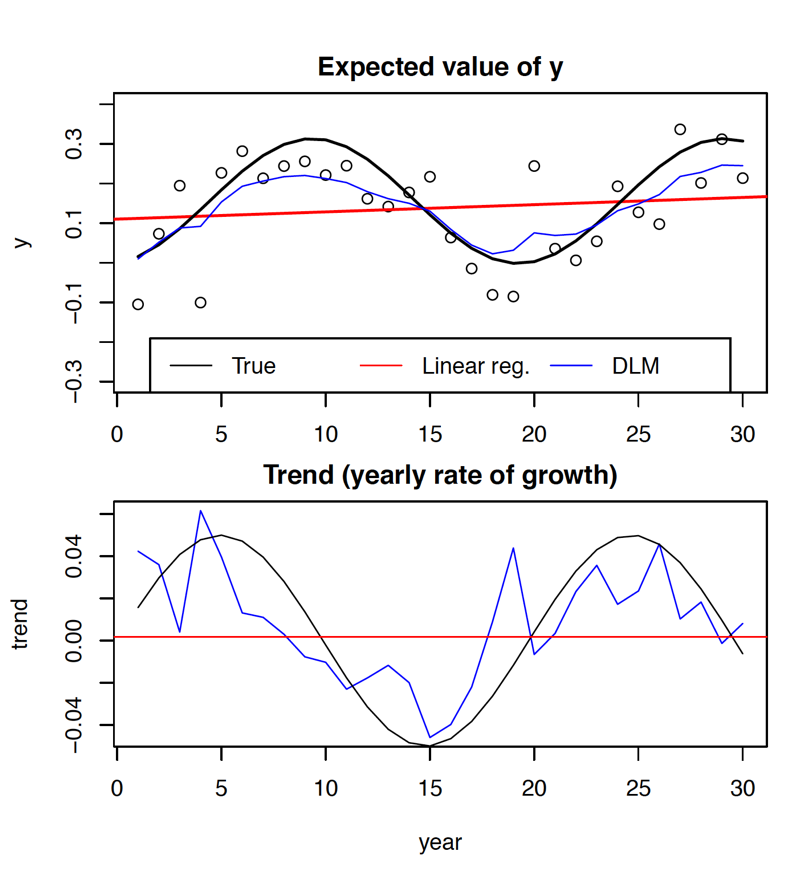
\includegraphics[width=2.69in,height=\textheight]{content/../media/image5.png}

}

\caption{This figure compares a trend analysis using a non-time-varying
trend (red line) via linear regression versus a trend analysis using a
time-varying trend (blue line). The black line is the true line we are
trying to estimate (with the red or blue line) and the dots in the top
panel are the observations of the black line. In the top plot, y is the
log-spawners. The trend in the lower plot is the yearly change in
log-spawners.}

\end{figure}

\hypertarget{code-to-fit-a-multivariate-dlm}{%
\subsection{Code to fit a multivariate
DLM}\label{code-to-fit-a-multivariate-dlm}}

The MARSS R package was used to fit multivariate DLMs to the log-spawner
counts (or indices in some cases). The package handles missing data
entered as NAs for missing years. The following example code fits 2
time-series via a multivariate DLM using the MARSS R package:

\begin{verbatim}
library(MARSS)
logspawners = log(matrix(c(1106, 1503, 853, 566, 251, 424, 783, 639, 566, 413, 1035, 890, 7348, 6880, 2699, 1096, NA, NA, NA, 1318, 1127, 472, 637, 869), 2,12, byrow=TRUE))
model=list(
  Q="equalvarcov", 
  R="diagonal and equal",
  U="unequal")
fit=MARSS(logspawners, model=model)
\end{verbatim}

\hypertarget{natural-origin-spawner-estimates}{%
\section{Natural-origin spawner
estimates}\label{natural-origin-spawner-estimates}}

For some populations, there were estimates of the fraction of total
natural spawners that were of natural-origin. However, for many
populations, these data were noisy and had many missing years. In
addition, the number of years with fraction natural-origin information
was often shorter than the years with total spawner counts. To estimate
a mean natural-origin spawner estimate, similar to the mean total
spawner estimate, the mean total spawner estimate was multiplied by a
smoothed estimate of the fraction natural-origin. The smoothed estimate
was produced by fitting a univariate DLM to the logit
\emph{z\textsubscript{t}} = log(\emph{f /}(1 \emph{− f} )) of the
fraction natural-origin estimates with a time-varying β. Specifically,
the following model was fit:

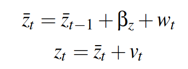
\includegraphics[width=0.63in,height=\textheight]{content/../media/image6.png}

The mean natural-origin spawner estimate at time \emph{t} was then
\emph{y}¯\emph{\textsubscript{t} exp(z}¯\emph{\textsubscript{t}
)/}(exp(\emph{z}¯\emph{\textsubscript{t} )}+ 1). Each time series of
fraction natural-origin from each population was fit independently (no
covariance assumed across populations). Missing values were allowed
within the fraction natural-origin time series and would be estimated by
the DLM, however no estimates were used more than 1-year before the
available data or 1-year after. For example, if the natural origin data
started in 2001, then the first DLM estimate would be for 2000. This
prevents the model from extrapolating too far outside the data.

\begin{figure}

{\centering 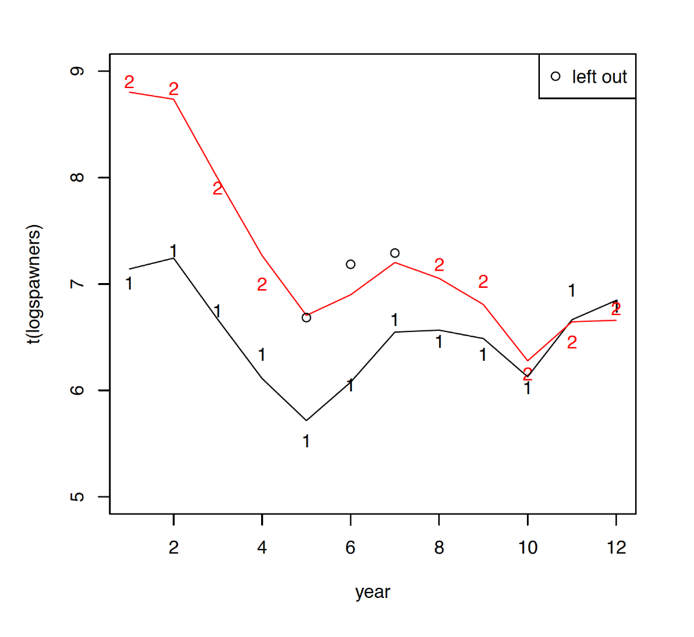
\includegraphics[width=2.31in,height=\textheight]{content/../media/image7.png}

}

\caption{The estimated mean log (spawners) using a multivariate DLM.
Notice that the information from the years when data are available for
time-series 1 are used to inform the estimate for time-series 2 for the
missing years (marked with a circle).}

\end{figure}

\hypertarget{summary-statistics}{%
\section{Summary statistics}\label{summary-statistics}}

The following summary statistics were reported for all ESUs: the mean
total spawner DLM estimates (from the multivariate DLM fit to the raw
total spawners time series in the ESU), the mean natural origin spawner
DLM estimates (the total spawner DLM estimate times the fraction natural
origin DLM estimate), and the raw (original data) total spawners and the
raw natural origin spawner estimates (raw total times fraction natural
origin). The definition of `spawner' with respect to age varied somewhat
across data sources and was dependent in some cases upon decisions made
by data providers. For Chinook salmon, jacks (males one year younger
than the model age) were included as spawners in most cases but
`mini-jacks' (males two or more years younger than the model age) were
never included. Jacks were not included for coho salmon. For steelhead,
only anadromous spawners were included.

These metrics are similar to statistics reported in prior viability
reports and provide a common set of relatively simple metrics for
comparison across all ESU/DPS and populations and with prior reports. In
most cases, there are also ESU/DPS-specific metrics that were developed
by technical recovery teams and/or included in recovery plans. Where
feasible, these metrics are also reported in the individual ESU/DPS
chapters.

\textbf{15-year trends. } A linear regression was fit to 15 years of the
mean natural origin spawner DLM estimates and the slope (trend)
reported. The 15-year time period was chosen to remain consistent with
prior viability reports and does not necessarily correspond to any peaks
or troughs in the time series.

\textbf{5-year geometric means. } 5-year geometric means
(\emph{y}\textsubscript{1}\emph{y}\textsubscript{2}\emph{y}\textsubscript{3}
\emph{y}\textsubscript{4}\emph{y}\textsubscript{5})\textsuperscript{(1\emph{/}5)}
were computed from the raw total natural spawner and natural origin
spawner DLM estimates. The raw data could have missing values in the
calculation, while the DLM estimates would not. For the raw estimates,
when there were missing values, the geometric mean was computed only
from the non-missing values. For example, if 3 values were available,
(\emph{y}\textsubscript{1}\emph{y}\textsubscript{2}\emph{y}\textsubscript{3})\textsuperscript{(1\emph{/}3)}
was reported.

\textbf{Average fraction natural origin. } These were computed over
5-year time frames from the raw estimates of fraction natural-origin.

\textbf{Productivity metric.} Because age of return data were not
consistently available across all ESUs and populations, a generic
productivity metric was computed as the mean natural-origin spawner DLM
estimate at year \emph{t} divided by the mean total spawner DLM estimate
at year \emph{t −} 3 for coho salmon and \emph{t −} 4 for all other
species. This metric was plotted for all years of available data.

\textbf{Harvest.} We compiled data on trends in the adult equivalent
exploitation rate for each ESU. This information was used to provide
some additional context for interpreting abundance trends, similar to
the environmental trend information we also report. It is important to
note that magnitude and trend of an exploitation rate cannot be
interpreted uncritically as a trend in level of risk from harvest.
Analyses relating exploitation rate to extinction risk or recovery
probability have been conducted in a quantitative way for several ESUs (
e.g., NMFS 2001; Ford \emph{et al.} 2007; NWFSC 2010) and qualitatively
for others (NMFS 2004). See specific sections for details.

\bookmarksetup{startatroot}

\hypertarget{esu-boundaries}{%
\chapter{ESU boundaries}\label{esu-boundaries}}

In the 2015 report NWFSC (2015) recommended a revision of the Lower
Columbia River Steelhead DPS and Upper Willamette River Steelhead DPS
boundaries. Specifically, that the Clackamas River winter steelhead
demographically independent population (DIP) originally included as part
of the Lower Columbia River DPS, instead be included in the Upper
Willamette River DPS. Genetic research published since 2015 further
supports the closer affinity of the Clackamas River winter-run steelhead
DIP to Upper Willamette River steelhead DPS populations rather than
Lower Columbia River steelhead DPS populations (Winans et al. 2018). We
believe that the rationale for revising the placement of the Clackamas
River winter steelhead DIP originally stated in the 2015 Status Review
is still accurate and appropriate and does not need further review or
revision.

\bookmarksetup{startatroot}

\hypertarget{upper-columbia-river-steelhead-dps}{%
\chapter{Upper Columbia River steelhead
DPS}\label{upper-columbia-river-steelhead-dps}}

The Upper Columbia Steelhead DPS includes all naturally spawned
anadromous \emph{O. mykiss} (steelhead) populations below natural and
manmade impassable barriers in streams in the Columbia River Basin
upstream from the Yakima River, Washington, to the US-Canada border, as
well as six artificial propagation programs (85 FR 81822 and Figure 10).
The Upper Columbia Steelhead DPS was originally listed under the ESA in
1997; it is currently designated as threatened.

\begin{figure}

{\centering 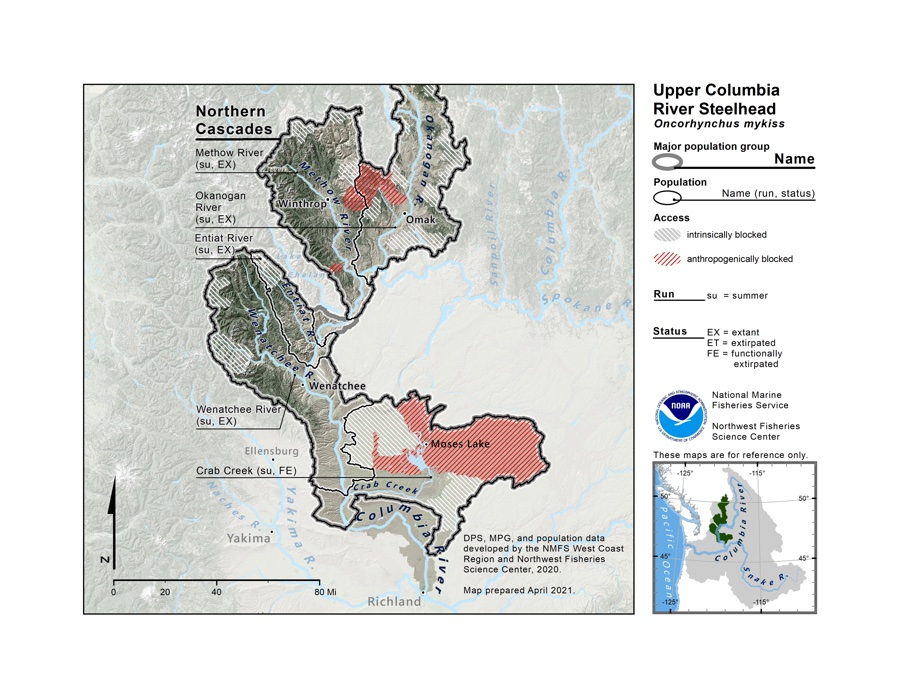
\includegraphics[width=3in,height=\textheight]{content/Interior_Columbia/../../media/image14.jpg}

}

\caption{\label{fig-UCR-steelhead-spawning-areas}Map of the Upper
steelhead DPS's spawning and rearing areas, illustrating populations and
major population groups.}

\end{figure}

NOAA Fisheries has defined DPSs of steelhead to include only the
anadromous members of this species (70 FR 67130). Our approach to
assessing the current viability of a steelhead DPS is based on
evaluating information on the abundance, productivity, spatial structure
and diversity of the anadromous component of the species (Good \emph{et
al}. 2005; 85 FR 81822). Many steelhead populations along the West Coast
of the U.S. co-occur with conspecific populations of resident rainbow
trout. We recognize that there may be situations where reproductive
contributions from resident rainbow trout may mitigate short-term
extinction risk for some steelhead DPSs (Good \emph{et al.} 2005); 85 FR
81822). We assume that any benefits to an anadromous population
resulting from the presence of a conspecific resident form will be
reflected in direct measures of the current viability of the anadromous
form.

\hypertarget{summary-of-previous-viability-conclusions}{%
\section{Summary of previous viability
conclusions}\label{summary-of-previous-viability-conclusions}}

\emph{2005}

The 2005 BRT cited low growth rate/productivity as the most serious risk
factor for the Upper Columbia River steelhead DPS (Good \emph{et al.}
2005). In particular, the BRT concluded that the extremely low
replacement rate of natural spawners highlighted in the 1998 review
continued through the subsequent brood cycle. The 2005 BRT assessment
also identified very low natural spawner abundance compared to interim
escapement objectives and high levels of hatchery spawners in natural
areas as contributing risk factors. The 2005 BRT report did note that
the number of naturally produced steelhead returning to spawn within
this DPS had increased over the levels reported in the 1998 status
review. As with the Mid-Columbia and Snake River DPS reviews, the 2005
BRT recognized that resident \emph{O. mykiss} were associated with
anadromous steelhead production areas for this DPS. The review stated
that the presence of resident \emph{O. mykiss} was considered a
mitigating factor by many of the BRT members in rating extinction risk.

\emph{2010}

The 2010 status review update reported that Upper Columbia steelhead
populations had increased in natural origin abundance in recent years,
but productivity levels remained low (Ford \emph{et al.} 2011). The
proportions of hatchery origin returns in natural spawning areas
remained extremely high across the DPS, especially in the Methow and
Okanogan River populations. The modest improvements in natural returns
that had been observed the years prior to the review were probably
primarily the result of several years of relatively good natural
survival in the ocean and tributary habitats. Tributary habitat actions
called for in the Upper Columbia Recovery Plan were anticipated to be
implemented over the next 25 years and the benefits of some of those
actions would require some time to be realized. Overall, the new
information considered did not indicate a change in the biological risk
category since the time of the last BRT status review.

\emph{2015}

Based on the review in 2015, Upper Columbia River steelhead populations
were determined to have increased relative to the low levels observed in
the 1990s, but natural origin abundance and productivity remained well
below viability thresholds for three out of the four populations (NWFSC
2015). The viability of the Wenatchee River steelhead population
continued to improve based on the additional years information available
for this review. The abundance and productivity viability rating for the
Wenatchee River exceeds the minimum threshold for 5\% extinction risk.
However, the overall DPS viability remains unchanged from the prior
review, remaining at high risk driven by low abundance and productivity
relative to viability objectives and diversity concerns. Application of
the criteria for abundance/productivity results in relatively coarse
scale ratings for each population. Across Interior Columbia DPSs, the
populations differ in the relative changes in survival or limiting
capacities that could lead to viable ratings. The required improvement
to improve the abundance/productivity estimates for Upper Columbia
Steelhead populations is at the high end of the range for all listed
Interior populations.

\hypertarget{description-of-new-data-available-for-this-review}{%
\section{Description of new data available for this
review}\label{description-of-new-data-available-for-this-review}}

The 2015 NWFSC status review (NWFSC 2015) evaluated the viability of the
Upper Columbia Steelhead DPS based on data series through cycle year
2013/2014 for each of the four extant populations, along with sampling
information collected at Priest Rapids Dam for the aggregate return to
the Upper Columbia Basin and Wells Dam (Methow and Okanogan populations
combined). Estimates generated using that methodology are currently
available through the 2018/2019 cycle years for each population.
Spawning escapement estimates are based on a run reconstruction model
incorporating annual dam counts, results of a three year radio tracking
program and estimates of broodstock and fisheries removals in various
reaches above Rock Island Dam. Estimates are generated by WDFW regional
staff (incorporating information from the Colville Tribal Fish \&
Wildlife Department) and are available through the StreamNet Coordinated
Assessment Project website. An updated approach for estimating
population level escapements has been initiated in recent years. That
approach uses mark/recapture statistics based on data generated from the
combination of systematic PIT tagging of a target proportion of the
returns passing Rock Island Dam (below all four population spawning
tributaries) and subsequent detections at arrays in each of the
tributaries (Waterhouse \emph{et al.} 2020). Comparisons of the results
from the updated approach with the methods used in prior years indicate
they generally produce compatible estimates for a given year.
Preliminary results are included in this assessment, in parallel to the
ongoing data collection based population assessments, with the
understanding that ongoing methodological and data evaluations will
result in a single approach to annual population enumeration in the
future.

\emph{Smolt to Adult Return and Recruits per Spawner Rates}

Smolt to Adult Return (SAR) estimates (Bonneville to Bonneville) for all
four Upper Columbia River Steelhead population data series are generated
by the Columbia River Data Access in Real Time (CBR, 2020) project using
PIT tag detections from all release locations within each population
basin (Columbia River DART, 2020). The indices represent cumulative
marine, nearshore and estuary survival. The SAR series includes
estimates for the range of brood years 2002-2015 (Figure 11). Over the
period of record, the geometric mean SAR for the Entiat, Methow and
Okanogan populations (\textasciitilde3\%) represents a low, but
reasonable marine survival (2\% is generally considered a minimal
replacement rate), with the Wenatchee SAR of \textasciitilde5\% being a
robust rate for a stable population. Recruits per Spawner (R/S) indices
are reported as available from the StreamNet Coordinated Assessments
data portal (StreamNet, 2020a). All populations in the ESU have low
(\textless{} 1.0) R/S values, implying that the natural replacement rate
is not keeping up with all sources of mortality across the life-cycle.

\begin{figure}

{\centering 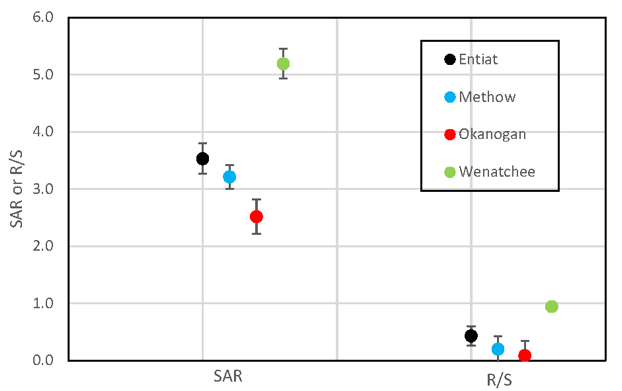
\includegraphics[width=2.07in,height=\textheight]{content/Interior_Columbia/../../media/image15.png}

}

\caption{\label{fig-UC-steelhead-Smolt-to-Adult}Smolt to Adult Return
and Recruits per Spawner for each of the populations in the ESU.
Geometric means of SAR and R/S are shown for each population, along with
the standard error of the estimate (whiskers represent +/- one standard
error). The time period included in the SAR or R/S indices is the past
20 years, depending on data availability.}

\end{figure}

\emph{Ocean Condition Indices}

Juvenile steelhead are more pelagic than salmon, heading off the
continental shelf soon after entering the ocean in the spring (Burgner
1992). Steelhead migrate seasonally across the North Pacific Ocean,
moving to the north and west in spring and to the south and east, across
the entire Pacific, from autumn through winter (Atcheson \emph{et al.}
2012). Thus, steelhead ocean survival may be impacted by different
factors than salmon. In fact, recent work has shown steelhead population
groupings from geographic regions have unique smolt survival trends that
appear to be driven by factors affecting them early in their ocean
residence despite steelhead smolts generally being larger than Pacific
salmon smolts when they enter the ocean and all making wide-ranging, off
the continental shelf migrations, rather than remaining more coastal, as
Pacific salmon smolts tend to do (Kendall \emph{et al.} 2017).

Aggregate annual returns of Columbia River steelhead are correlated with
a range of ocean condition indices including measures of broad scale
physical conditions, local biological indicators, and local physical
factors (Peterson \emph{et al.} 2014a). Work is ongoing to relate
indices of ocean condition to steelhead populations up and down the West
Coast. Steelhead marine survival seems to be related to ocean surface
temperature in the first summer of ocean entry, and populations respond
similarly to spatial patterns of ocean conditions at a rough grain of
250km between ocean entry points (Kendall \emph{et al.} 2017).
Therefore, broad spatial patterns of ocean conditions may not capture
the finer spatial scale of response that steelhead seem to exhibit.

Indicators of ocean condition are highly correlated with each other, and
exhibit strong temporal autocorrelation (Figure 129, (Peterson \emph{et
al.} 2019)). As a result, when indicators point to conditions that
result in poor ocean productivity for salmonid populations, they do so
as a suite of indicators, and for runs of `good' or `bad' years (see
Habitat chapter). Historically, ocean conditions cycled between periods
of high and low productivity. However, global climate change is likely
to disrupt this pattern, in general, leading to a preponderance of low
productivity years, with an unknown temporal distribution (Crozier
\emph{et al.} 2019b). Recent (2015-2019) ensemble ocean indicators
rankings include four of the worst seven years in the past 20, meaning
that an entire salmon or steelhead generation could have been subjected
to poor ocean productivity conditions.

\hypertarget{abundance-and-productivity}{%
\section{Abundance and productivity}\label{abundance-and-productivity}}

Updated data series on spawner abundance, age structure and hatchery
wild proportions were used to generate current assessments of abundance
and productivity at the population level. Evaluations were done using
both a set of metrics corresponding to those used in prior ESA Status
Reviews as well as a set corresponding to the specific viability
criteria based on ICTRT recommendations for this DPS. The standard
Status Review metrics were consistently done across all ESUs and DPSs to
facilitate comparisons across domains. Assessments using the ICTRT
metrics are described in the TRT and Recovery Plan Criteria section
below. The ICTRT abundance and productivity metrics are measured over
longer time frames to dampen the effects of annual variations and they
use annual natural origin age composition to calculate brood year
recruitment when sampling levels meet regional fishery agency criteria.

The most recent estimates (5-year geometric mean) of total and
natural-origin spawner abundance have declined dramatically, erasing
gains observed over the past two decades for all four populations
(Figure 12, Table 6). Recent declines are persistent and large enough to
result in small, but negative 15-year trends in abundance for all four
populations (Table 7). Updated spawner estimation methods show a strong
concordance with existing methods (Figure 13), which is extremely
encouraging as the estimation process based on detecting tags from a
run-at-large tagging program is a very robust approach to monitoring
across the DPS. Annual brood year return-per-spawner estimates have been
well below replacement in recent years for all four populations. The
return per spawner estimates summarized in Figure 14 are ratios of the
estimated natural origin returns produced from spawners in each brood
year, under the assumption that both hatchery and natural origin fish
contribute to production as parent spawners. All populations are
consistently exhibiting natural production rates well below replacement,
and natural production has also declined consistently, resulting in an
increasing fraction of hatchery fish on the spawning grounds each year.

The required improvement to increase abundance and productivity for
Upper Columbia Steelhead populations is at the high end of the range for
all listed Interior populations. Using the R/S and SAR indicators by
population (Figure 15), it is possible to generate an indicator of fresh
water productivity (FWPI) as a ratio of R/S and SAR. This quantity can
be thought of as an indicator of smolts per spawner, and thus, the
overall population productivity in the freshwater environment. FWPI for
Upper Columbia steelhead populations are very low
(\textless\textless100, Figure 15), confirming areas of recovery action
focus such as pre-spawn mortality and juvenile rearing habitat
condition, as well as mainstem migratory impacts as the SAR are based on
Bonneville to Bonneville tag detections and the R/S are based on
spawning ground recruits. The initial ICTRT assessment of
abundance/productivity gaps resulted in a pattern similar to that
indicated by the long-term productivity metrics (ICTRT 2007,). The
Wenatchee River population has somewhat higher productivity (SAR, R/S,
and FWPI) than the remaining populations in the DPS, but still falls
into a high risk category due to the recent downward trend in both
abundance and productivity.

\begin{figure}

\begin{minipage}[t]{\linewidth}

{\centering 

\raisebox{-\height}{

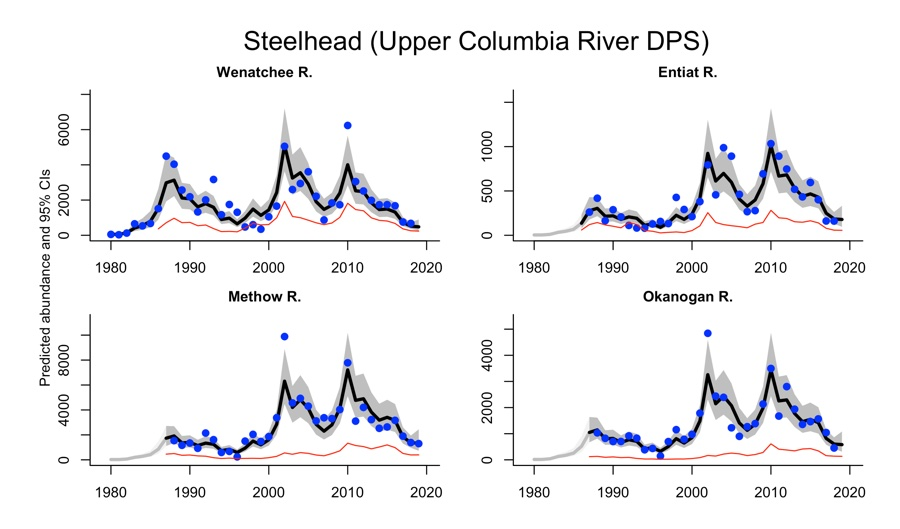
\includegraphics[width=3in,height=\textheight]{content/Interior_Columbia/../../media/image16.jpg}

}

}

\subcaption{\label{fig-UC-steelhead-smoothed-trends-1}Traditionally
generated spawner abundance}
\end{minipage}%
\newline
\begin{minipage}[t]{\linewidth}

{\centering 

\raisebox{-\height}{

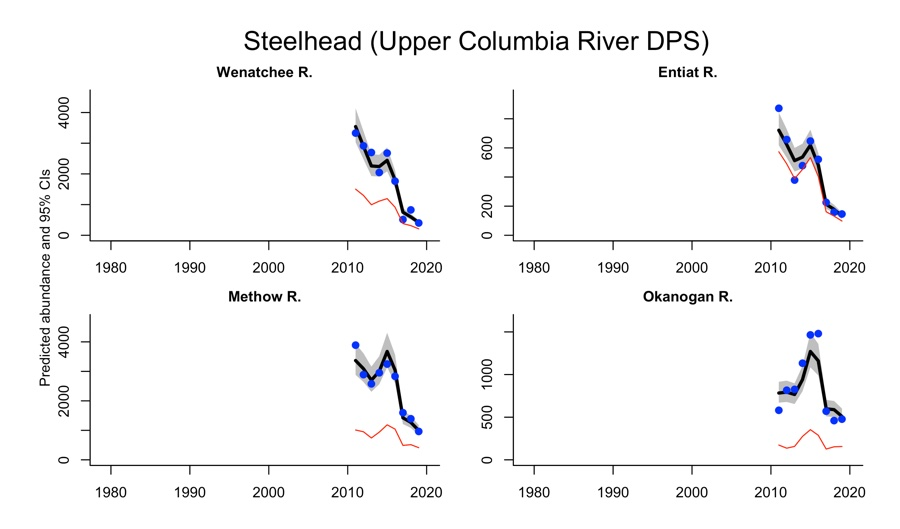
\includegraphics[width=3in,height=\textheight]{content/Interior_Columbia/../../media/image17.jpg}

}

}

\subcaption{\label{fig-UC-steelhead-smoothed-trends-2}PIT tag based}
\end{minipage}%

\caption{\label{fig-UC-steelhead-smoothed-trends}Smoothed trend in
estimated total (thick black line, with 95\% confidence internal in
gray) and natural (thin red line) population spawning abundance. In
portions of a time series where a population has no annual estimates but
smoothed spawning abundance is estimated from correlations with other
populations the smoothed estimate is shown in light gray. Points show
the annual raw spawning abundance estimates. For some trends the
smoothed estimate may be influenced by earlier data points not included
in the plot. Upper panel is the traditionally generated spawner
abundance timeseries for each population. The lower panel is the PIT tag
based population estimates based on a tag detections within each
population watershed relative to tagging the aggregate Upper Columbia
River run at large.}

\end{figure}

\begin{figure}

{\centering 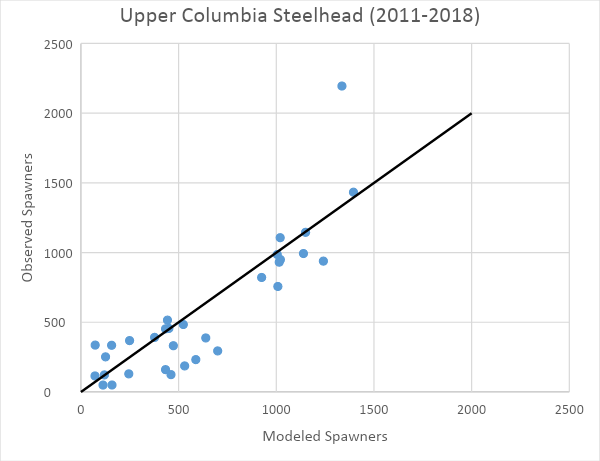
\includegraphics[width=2in,height=\textheight]{content/Interior_Columbia/../../media/image18.png}

}

\caption{\label{fig-UC-steelhead-one-to-one}Estimate spawners relative
to observed spawners across all four populations for all years where
both measures exist. Black line represents the expected 1:1 relationship
if the run-at-large tagging based, model estimated population measures
match the current redd survey based measures.}

\end{figure}

\begin{figure}

{\centering 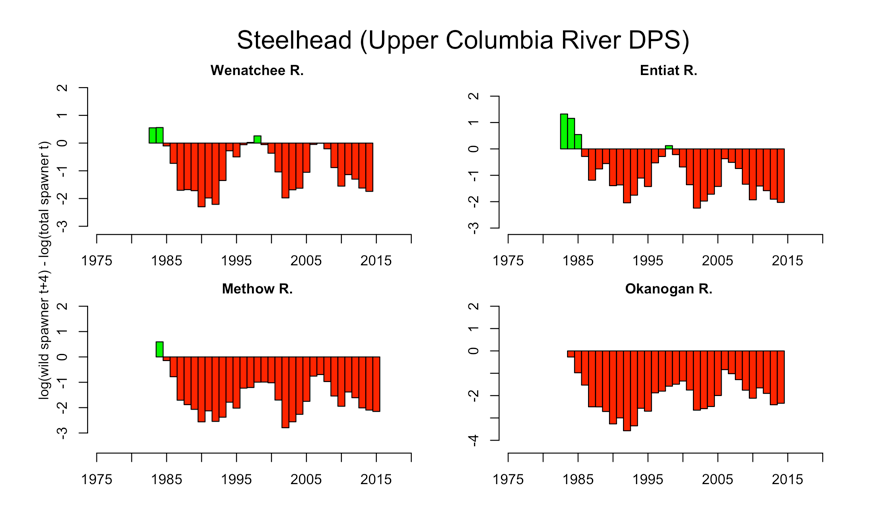
\includegraphics[width=2.92in,height=\textheight]{content/Interior_Columbia/../../media/image19.png}

}

\caption{\label{fig-UC-Spr-Chinook-productivity-trends}Trends in
population productivity, estimated as the log of the smoothed natural
spawning abundance in year \emph{t} divided by the smoothed natural
spawning abundance in year \emph{t}- 4. Spawning years on x axis.}

\end{figure}

\begin{figure}

{\centering 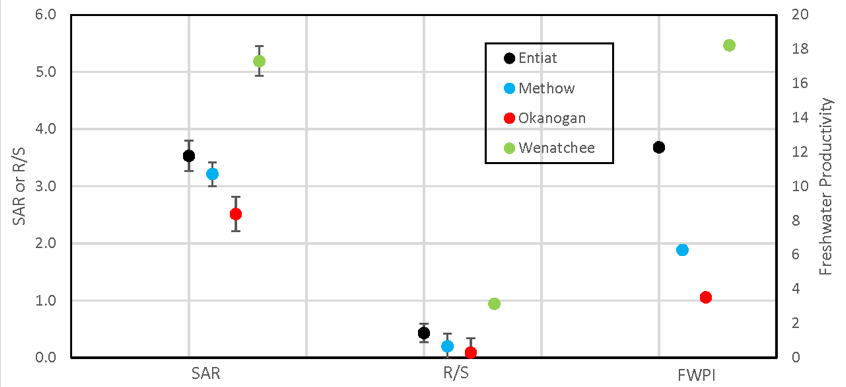
\includegraphics[width=2.82in,height=\textheight]{content/Interior_Columbia/../../media/image20.png}

}

\caption{\label{fig-UC-Spr-Chinook-Smolt-to-Adult-Productivity}Smolt to
Adult Return, Recruits per Spawner, and Freshwater Productivity Index
(FWPI) for each of the populations in the DPS. Geometric means of SAR
and R/S are shown for each population, along with the standard error of
the estimate (whiskers represent +/- one standard error). The time
period included in the SAR or R/S indices is the past 20 years,
depending on data availability. The FWPI is constructed as a ratio of
the geomean R/S and SAR, and can be thought of as a measure of smolts
per spawner.}

\end{figure}

\begin{longtable}[]{@{}
  >{\raggedright\arraybackslash}p{(\columnwidth - 16\tabcolsep) * \real{0.1215}}
  >{\raggedright\arraybackslash}p{(\columnwidth - 16\tabcolsep) * \real{0.1028}}
  >{\raggedright\arraybackslash}p{(\columnwidth - 16\tabcolsep) * \real{0.1121}}
  >{\raggedright\arraybackslash}p{(\columnwidth - 16\tabcolsep) * \real{0.1121}}
  >{\raggedright\arraybackslash}p{(\columnwidth - 16\tabcolsep) * \real{0.1121}}
  >{\raggedright\arraybackslash}p{(\columnwidth - 16\tabcolsep) * \real{0.1121}}
  >{\raggedright\arraybackslash}p{(\columnwidth - 16\tabcolsep) * \real{0.1121}}
  >{\raggedright\arraybackslash}p{(\columnwidth - 16\tabcolsep) * \real{0.1121}}
  >{\raggedright\arraybackslash}p{(\columnwidth - 16\tabcolsep) * \real{0.0841}}@{}}
\caption{Table . 5-year mean of fraction natural origin (sum of all
estimates divided by the number of estimates). Blanks mean no estimate
available in that 5-year range.}\tabularnewline
\toprule()
\begin{minipage}[b]{\linewidth}\raggedright
Population
\end{minipage} & \begin{minipage}[b]{\linewidth}\raggedright
MPG
\end{minipage} & \begin{minipage}[b]{\linewidth}\raggedright
1990-1994
\end{minipage} & \begin{minipage}[b]{\linewidth}\raggedright
1995-1999
\end{minipage} & \begin{minipage}[b]{\linewidth}\raggedright
2000-2004
\end{minipage} & \begin{minipage}[b]{\linewidth}\raggedright
2005-2009
\end{minipage} & \begin{minipage}[b]{\linewidth}\raggedright
2010-2014
\end{minipage} & \begin{minipage}[b]{\linewidth}\raggedright
2015-2019
\end{minipage} & \begin{minipage}[b]{\linewidth}\raggedright
\% Change
\end{minipage} \\
\midrule()
\endfirsthead
\toprule()
\begin{minipage}[b]{\linewidth}\raggedright
Population
\end{minipage} & \begin{minipage}[b]{\linewidth}\raggedright
MPG
\end{minipage} & \begin{minipage}[b]{\linewidth}\raggedright
1990-1994
\end{minipage} & \begin{minipage}[b]{\linewidth}\raggedright
1995-1999
\end{minipage} & \begin{minipage}[b]{\linewidth}\raggedright
2000-2004
\end{minipage} & \begin{minipage}[b]{\linewidth}\raggedright
2005-2009
\end{minipage} & \begin{minipage}[b]{\linewidth}\raggedright
2010-2014
\end{minipage} & \begin{minipage}[b]{\linewidth}\raggedright
2015-2019
\end{minipage} & \begin{minipage}[b]{\linewidth}\raggedright
\% Change
\end{minipage} \\
\midrule()
\endhead
Wenatchee R. & North Cascades & 527 (1847) & 264 (741) & 774 (2319) &
684 (1857) & 1497 (2774) & 554 (1104) & -63 (-60) \\
Entiat R. & North Cascades & 68 (134) & 38 (201) & 110 (491) & 102 (462)
& 203 (688) & 92 (280) & -55 (-59) \\
Methow R. & North Cascades & 210 (1206) & 97 (937) & 435 (4255) & 523
(3599) & 829 (3833) & 595 (1954) & -28 (-49) \\
Okanogan R. & North Cascades & 65 (678) & 25 (526) & 124 (2178) & 184
(1328) & 404 (2122) & 223 (1020) & -45 (-52) \\
\bottomrule()
\end{longtable}

\begin{longtable}[]{@{}
  >{\raggedright\arraybackslash}p{(\columnwidth - 6\tabcolsep) * \real{0.2267}}
  >{\raggedright\arraybackslash}p{(\columnwidth - 6\tabcolsep) * \real{0.2400}}
  >{\raggedright\arraybackslash}p{(\columnwidth - 6\tabcolsep) * \real{0.2400}}
  >{\raggedright\arraybackslash}p{(\columnwidth - 6\tabcolsep) * \real{0.2667}}@{}}
\caption{Table . Viability assessments for extant Upper Columbia
Steelhead DPS populations. Natural spawning abundance: most recent 10
year geometric mean (range). ICTRT productivity: 20 year geometric mean
for parent escapements below 75\% of population threshold. Current
abundance and productivity estimates are geometric means. Range in
annual abundance, standard error and number of qualifying estimates for
productivities in parentheses..}\tabularnewline
\toprule()
\begin{minipage}[b]{\linewidth}\raggedright
Population
\end{minipage} & \begin{minipage}[b]{\linewidth}\raggedright
MPG
\end{minipage} & \begin{minipage}[b]{\linewidth}\raggedright
1990-2005
\end{minipage} & \begin{minipage}[b]{\linewidth}\raggedright
2004-2019
\end{minipage} \\
\midrule()
\endfirsthead
\toprule()
\begin{minipage}[b]{\linewidth}\raggedright
Population
\end{minipage} & \begin{minipage}[b]{\linewidth}\raggedright
MPG
\end{minipage} & \begin{minipage}[b]{\linewidth}\raggedright
1990-2005
\end{minipage} & \begin{minipage}[b]{\linewidth}\raggedright
2004-2019
\end{minipage} \\
\midrule()
\endhead
Wenatchee R. & North Cascades & 0.06 (0.01, 0.12) & -0.1 (-0.15,
-0.06) \\
Entiat R. & North Cascades & 0.11 (0.05, 0.17) & -0.06 (-0.11, -0.01) \\
Methow R. & North Cascades & 0.11 (0.06, 0.17) & -0.05 (-0.1, -0.01) \\
Okanogan R. & North Cascades & 0.1 (0.05, 0.16) & -0.06 (-0.11,
-0.02) \\
\bottomrule()
\end{longtable}

\hypertarget{spatial-structure-and-diversity}{%
\section{Spatial structure and
diversity}\label{spatial-structure-and-diversity}}

With the exception of the Okanogan population, the upper Columbia River
populations were rated as low risk for spatial structure. The high risk
ratings for diversity are largely driven by high levels of hatchery
spawners within natural spawning areas and lack of genetic diversity
among the populations. The basic major life history patterns (summer
A-run type, tributary and mainstem spawning/rearing patterns, and the
presence of resident populations and subpopulations) appear to be
present. All of the populations were rated at high risk for current
genetic characteristics by the ICTRT. Genetics samples taken in the
1980s indicate little differentiation within populations in the upper
Columbia River DPS. More recent studies within the Wenatchee River basin
have found differences between samples from the Peshastin River,
believed to be relatively isolated from hatchery spawning, and those
from other reaches within the Wenatchee. This suggests that there may
have been a higher level of within and among population diversity prior
to the advent of major hatchery releases (Seamons \emph{et al.} 2012).
Genetic studies based on sampling in the Wenatchee as well as other
Upper Columbia River steelhead population tributaries are underway and
should allow for future analyses of current genetic structure and any
impacts of changing hatchery release practices.

Hatchery-origin returns continue to constitute a high fraction of total
spawners in natural spawning areas for this DPS (Table 8). The estimated
proportion of natural-origin spawners has increased consistently since
the late 1990s for all four populations (Figure 16). Natural-origin
proportions were the highest in the Wenatchee River (58\%). Although
increasing, natural origin proportions in the Methow and Okanogan rivers
remained at low levels. There are currently direct releases of hatchery
origin juveniles in three of the four populations, the exception being
the Entiat River. Based on PIT detections, hatchery origin spawners in
the Entiat River include stray hatchery returns from releases into the
Wenatchee River (Hillman \emph{et al.} 2015). Reproductive effectiveness
studies on the Wenatchee population indicate that hatchery-hatchery
matings have dramatically reduced fitness compared to matings among
natural-origin fish (Ford \emph{et al.} 2016), reinforcing the weight
the ICTRT placed on the presence of hatchery origin spawners in the
Spatial Structure and Diversity metric.

\begin{figure}

{\centering 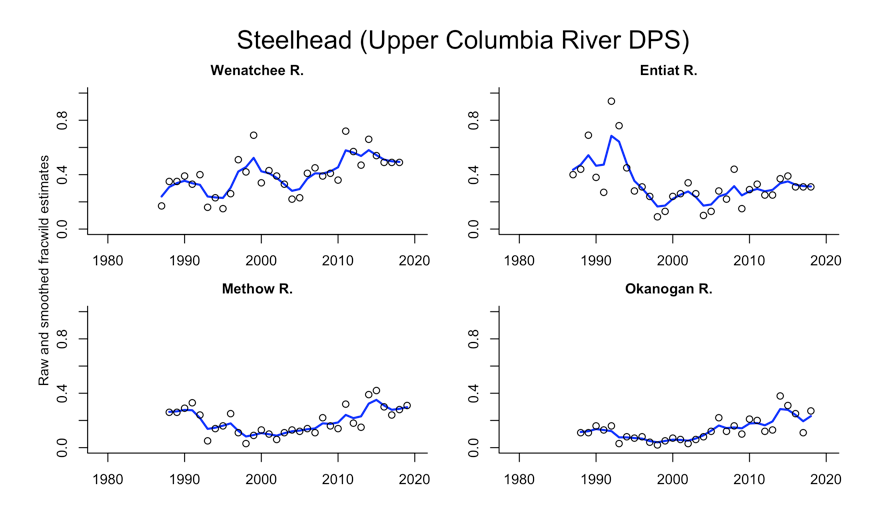
\includegraphics[width=2.92in,height=\textheight]{content/Interior_Columbia/../../media/image21.png}

}

\caption{\label{fig-UC-steelhead-smoothed-frac-wild}Smoothed trend in
the estimated fraction of the natural spawning population consisting of
fish if natural origin. Points show the annual raw estimates.}

\end{figure}

\begin{longtable}[]{@{}
  >{\raggedright\arraybackslash}p{(\columnwidth - 10\tabcolsep) * \real{0.1948}}
  >{\raggedright\arraybackslash}p{(\columnwidth - 10\tabcolsep) * \real{0.1558}}
  >{\raggedright\arraybackslash}p{(\columnwidth - 10\tabcolsep) * \real{0.1558}}
  >{\raggedright\arraybackslash}p{(\columnwidth - 10\tabcolsep) * \real{0.1558}}
  >{\raggedright\arraybackslash}p{(\columnwidth - 10\tabcolsep) * \real{0.1558}}
  >{\raggedright\arraybackslash}p{(\columnwidth - 10\tabcolsep) * \real{0.1558}}@{}}
\caption{Table . Upper Columbia Steelhead DPS Steelhead population risk
ratings integrated across the four VSP parameters. Viability key: HV,
highly viable; V, viable; M, maintained; and HR, high risk (does not
meet viability criteria).}\tabularnewline
\toprule()
\begin{minipage}[b]{\linewidth}\raggedright
Population
\end{minipage} & \begin{minipage}[b]{\linewidth}\raggedright
1995-1999
\end{minipage} & \begin{minipage}[b]{\linewidth}\raggedright
2000-2004
\end{minipage} & \begin{minipage}[b]{\linewidth}\raggedright
2005-2009
\end{minipage} & \begin{minipage}[b]{\linewidth}\raggedright
2010-2014
\end{minipage} & \begin{minipage}[b]{\linewidth}\raggedright
2015-2019
\end{minipage} \\
\midrule()
\endfirsthead
\toprule()
\begin{minipage}[b]{\linewidth}\raggedright
Population
\end{minipage} & \begin{minipage}[b]{\linewidth}\raggedright
1995-1999
\end{minipage} & \begin{minipage}[b]{\linewidth}\raggedright
2000-2004
\end{minipage} & \begin{minipage}[b]{\linewidth}\raggedright
2005-2009
\end{minipage} & \begin{minipage}[b]{\linewidth}\raggedright
2010-2014
\end{minipage} & \begin{minipage}[b]{\linewidth}\raggedright
2015-2019
\end{minipage} \\
\midrule()
\endhead
Wenatchee R. & 0.41 & 0.34 & 0.38 & 0.56 & 0.50 \\
Entiat R. & 0.21 & 0.24 & 0.24 & 0.30 & 0.33 \\
Methow R. & 0.13 & 0.11 & 0.15 & 0.24 & 0.31 \\
Okanogan R. & 0.05 & 0.06 & 0.14 & 0.21 & 0.24 \\
\bottomrule()
\end{longtable}

\hypertarget{non-treaty-harvest}{%
\section{Non-treaty Harvest}\label{non-treaty-harvest}}

Steelhead were historically taken in tribal and non-tribal gillnet
fisheries, and in recreational fisheries in the mainstem Columbia River
and in tributaries. In the 1970s, retention of steelhead in non-treaty
commercial fisheries was prohibited, and in the mid 1980s, tributary
recreational fisheries in Washington adopted mark-selective regulations.
There is incidental mortality associated with mark-selective
recreational fisheries. Sport fisheries targeting hatchery run steelhead
occur in the mainstem Columbia River and in several Upper Columbia River
tributaries. In recent years, Upper Columbia River exploitation rates
have been stable at around 1.5\%. As of 2012, rates are estimated over
two management intervals per year, Fall and Winter/Spring/Summer (Figure
17).

Figure . Harvest rates for non-treaty Upper Columbia steelhead. As of
2012, reporting is generated across two management periods, Fall (blue
line) and Winter/Spring/Summer (orange line), previously harvest rate
reporting was across all of the calendar year. TAC 2020.

\hypertarget{biological-viability-relative-to-recovery-goals}{%
\section{Biological viability relative to recovery
goals}\label{biological-viability-relative-to-recovery-goals}}

NOAA Fisheries adopted a recovery plan for upper Columbia River spring
Chinook salmon and steelhead in 2007 (FR 72 \#194, 57303−57307). The
plan was developed by the Upper Columbia Salmon Recovery Board (UCSRB)
and is available at:
https://www.fisheries.noaa.gov/resource/document/recovery-plan-upper-columbia-spring-chinook-salmon-and-steelhead.

Achieving recovery (delisting) of each ESU via sufficient improvement in
abundance, productivity, spatial structure, and diversity is the longer
term goal of the UC Recovery Plan. The UC Recovery Plan includes
specific quantitative criteria expressed relative to population
viability curves (ICTRT 2007). It includes two quantitative criteria for
assessing the viability of the steelhead DPS against the recovery
objective: ``The 12-year geometric mean (representing approximately
three generations) of abundance and productivity of naturally produced
steelhead within the Wenatchee, Entiat, and Methow populations must
reach a level that would have not less than a 5\% extinction-risk
(viability) over a 100 year period'' and ``at a minimum, the Upper
Columbia Steelhead DPS will maintain at least 3,000 naturally produced
spawners and a spawner:spawner ratio greater than 1:1 distributed among
the three populations.'' The minimum number of naturally produced
spawners (expressed as 12-year geometric means) should exceed 1,000 each
for the Wenatchee and Methow river populations and 500 each for the
Entiat and Okanogan river populations. The plan also established minimum
productivity thresholds. These natural spawner abundance criteria
replace the interim targets referenced in the 2005 BRT report. The
12-year geometric mean productivity should exceed 1.1 spawners per
parent spawner for the two larger populations (Wenatchee and Methow
Rivers), and 1.2 for the smaller Entiat River and Okanogan populations.

The ICTRT had recommended that at least two of the four extant
populations be targeted for highly viable status (less than 1\% risk of
extinction over 100 years) because of the relatively low number of
extant populations remaining in the DPS. The UC Recovery Plan adopted an
alternative approach for addressing the limited number of populations in
the DPS---5\% or less risk of extinction for at least three of the four
extant populations.

The UC Recovery Plan also calls for ``\ldots{} restoring the
distribution of naturally produced spring Chinook salmon and steelhead
to previously occupied areas where practical, and conserving their
genetic and phenotypic diversity.'' Specific criteria included in the UC
Recovery Plan reflect a combination of the criteria recommended by the
ICTRT (ICTRT 2007) and an earlier pre-TRT analytical project (Ford
\emph{et al.} 2001). The plan incorporates spatial structure criteria
specific to each steelhead population. For the Wenatchee River
population, the criteria require observed natural spawning in four of
the five major spawning areas as well as in at least one of the minor
spawning areas downstream of Tumwater Dam. In the Methow River, natural
spawning should be observed in three major spawning areas. In each case,
the major spawning areas should include a minimum of 5\% of the total
return to the system or 20 redds, whichever is greater. In the Entiat,
natural spawning should be observed in both historical major spawning
areas, with a distribution criteria similar to the Methow. In the
Okanogan, natural spawning should be observed within the two major
spawning areas and within at least two of the five minor spawning areas,
with a numerical distribution similar to the Methow, across the minor
spawning areas. The plan incorporates criteria for spatial structure and
diversity adopted from the ICTRT viability report. The mean score for
the three metrics representing natural rates and spatially mediated
processes should result in a moderate or lower risk in each of the three
populations and all threats defined as high risk must be addressed. In
addition, the mean score for the eight ICTRT metrics tracking natural
levels of variation should result in a moderate or lower risk score at
the population level.

Table . 5-year geometric mean of raw natural origin spawner counts. This
is the raw total spawner count times the fraction natural origin
estimate, if available. In parentheses, 5-year geometric mean of raw
total spawner counts is shown. A value only in parentheses means that a
total spawner count was available but no or only one estimate of natural
origin spawners available. The geometric mean was computed as the
product of counts raised to the power 1 over the number of counts
available (2 to 5). A minimum of 2 values were used to compute the
geometric mean. Percent change between the most recent two 5-year
periods is shown on the far right.

Population

Abundance and productivity metrics

Spatial structure and diversity metrics

Overall Risk Rating

ICTRT minimum

Natural spawning

ICTRT productivity

Integrated A/P risk

Natural processes

Diversity risk

Integrated SS/D risk

Wenatchee River

1,000

931

(sd. 667)

0.95

(0.06, 13/20)

Moderate

Low

High

High

High

Entiat River

500

140

(sd. 89)

0.433

(0.17, 20/20)

High

Moderate

High

High

High

Methow River

1,000

703

(sd. 297)

0.20

(0.22, 12/20)

High

Low

High

High

High

Okanogan River

750

297

(sd. 189)

0.09

(0.25, 19/20)

High

High

High

High

High

: Table . 5-year geometric mean of raw natural origin spawner counts.
This is the raw total spawner count times the fraction natural origin
estimate, if available. In parentheses, 5-year geometric mean of raw
total spawner counts is shown. A value only in parentheses means that a
total spawner count was available but no or only one estimate of natural
origin spawners available. The geometric mean was computed as the
product of counts raised to the power 1 over the number of counts
available (2 to 5). A minimum of 2 values were used to compute the
geometric mean. Percent change between the most recent two 5-year
periods is shown on the far right.

\hypertarget{updated-biological-risk-summary}{%
\section{Updated biological risk
summary}\label{updated-biological-risk-summary}}

Given the recent changes in hatchery practices in the Wenatchee River
and the potential for reduced hatchery contributions or increased
spatial separation of hatchery vs.~natural origin spawners, it is
possible that genetic composition could trend towards patterns
consistent with strong natural selection influences in the future.
Ongoing genetic sampling and analysis could provide information in the
future to determine if the diversity risk is abating. The proportions of
hatchery-origin returns in natural spawning areas remain high across the
DPS, especially in the Methow and Okanogan river populations. Tributary
habitat actions called for in the Upper Columbia Recovery Plan are
anticipated to be implemented over the next 25 years and the benefits of
some of those actions will require some time to be realized.

The most recent estimates (5-year geometric mean) of total and
natural-origin spawner abundance have declined since the last report,
largely erasing gains observed over the past two decades for all four
populations (Figure 12, Table 6). Recent declines are persistent and
large enough to result in small, but negative 15-year trends in
abundance for all four populations (Table 7). The abundance and
productivity viability rating for the Wenatchee River exceeds the
minimum threshold for 5\% extinction risk. The overall DPS viability
remains unchanged from the prior review, remaining at high risk driven
by low abundance and productivity relative to viability objectives and
diversity concerns (Table 9).

\begin{longtable}[]{@{}
  >{\raggedright\arraybackslash}p{(\columnwidth - 10\tabcolsep) * \real{0.2500}}
  >{\raggedright\arraybackslash}p{(\columnwidth - 10\tabcolsep) * \real{0.1528}}
  >{\raggedright\arraybackslash}p{(\columnwidth - 10\tabcolsep) * \real{0.1389}}
  >{\raggedright\arraybackslash}p{(\columnwidth - 10\tabcolsep) * \real{0.0833}}
  >{\raggedright\arraybackslash}p{(\columnwidth - 10\tabcolsep) * \real{0.1528}}
  >{\raggedright\arraybackslash}p{(\columnwidth - 10\tabcolsep) * \real{0.1667}}@{}}
\caption{Table . 15-year trends in log natural origin spawner abundance
computed from a linear regression applied to the smoothed natural origin
spawner log abundance estimate. Only populations with at least 4 wild
spawner estimates and with at least 2 data points (actual data not
estimates) in the first 5 years and last 5 years of the 15-year ranges
are shown.}\tabularnewline
\toprule()
\begin{minipage}[b]{\linewidth}\raggedright
\end{minipage} & \begin{minipage}[b]{\linewidth}\raggedright
\end{minipage} & \begin{minipage}[b]{\linewidth}\raggedright
\textbf{ Spatial struc ture/di versity risk}
\end{minipage} & \begin{minipage}[b]{\linewidth}\raggedright
\end{minipage} & \begin{minipage}[b]{\linewidth}\raggedright
\end{minipage} & \begin{minipage}[b]{\linewidth}\raggedright
\end{minipage} \\
\midrule()
\endfirsthead
\toprule()
\begin{minipage}[b]{\linewidth}\raggedright
\end{minipage} & \begin{minipage}[b]{\linewidth}\raggedright
\end{minipage} & \begin{minipage}[b]{\linewidth}\raggedright
\textbf{ Spatial struc ture/di versity risk}
\end{minipage} & \begin{minipage}[b]{\linewidth}\raggedright
\end{minipage} & \begin{minipage}[b]{\linewidth}\raggedright
\end{minipage} & \begin{minipage}[b]{\linewidth}\raggedright
\end{minipage} \\
\midrule()
\endhead
& & \textbf{Very low} & \begin{minipage}[t]{\linewidth}\raggedright
\begin{itemize}
\tightlist
\item
  *Lo w**
\end{itemize}
\end{minipage} & \textbf{Mo derate} & \textbf{High} \\
\textbf{Abundance/}

\textbf{productivity risk} & \textbf{Very low}

(\textless1\%) & \textbf{HV} & \textbf{H V} & \textbf{V} & \textbf{M} \\
& \textbf{Low}

(1--5\%) & \textbf{V} & \textbf{ V} & \textbf{V} & \textbf{M} \\
& \textbf{Mo derate}

(6--25\%) & \textbf{M} & \textbf{ M} & \textbf{M} & \textbf{HR}

\textbf{We natchee} \\
& \textbf{High}

(\textgreater25\%) & \textbf{HR} & \textbf{H R} & \textbf{HR} &
\begin{minipage}[t]{\linewidth}\raggedright
\textbf{HR}

\begin{itemize}
\item
  *Entiat**
\item
  *Methow**
\end{itemize}

\textbf{O kanogan}
\end{minipage} \\
\bottomrule()
\end{longtable}

\bookmarksetup{startatroot}

\hypertarget{upper-columbia-river-spring-chinook-salmon-esu}{%
\chapter{Upper Columbia River spring Chinook salmon
ESU}\label{upper-columbia-river-spring-chinook-salmon-esu}}

The Upper Columbia Spring-Run Chinook salmon ESU includes naturally
spawning spring-run Chinook salmon in the major tributaries entering the
Columbia River upstream of Rock Island Dam and associated hatchery
programs (85 FR 81822; Figure~\ref{fig-UCR-Spr-Chinook-spawning-areas}).
The ESU was listed as Endangered under the ESA in 1999 (affirmed in
2005, 2012 and 2016).

\begin{figure}

{\centering 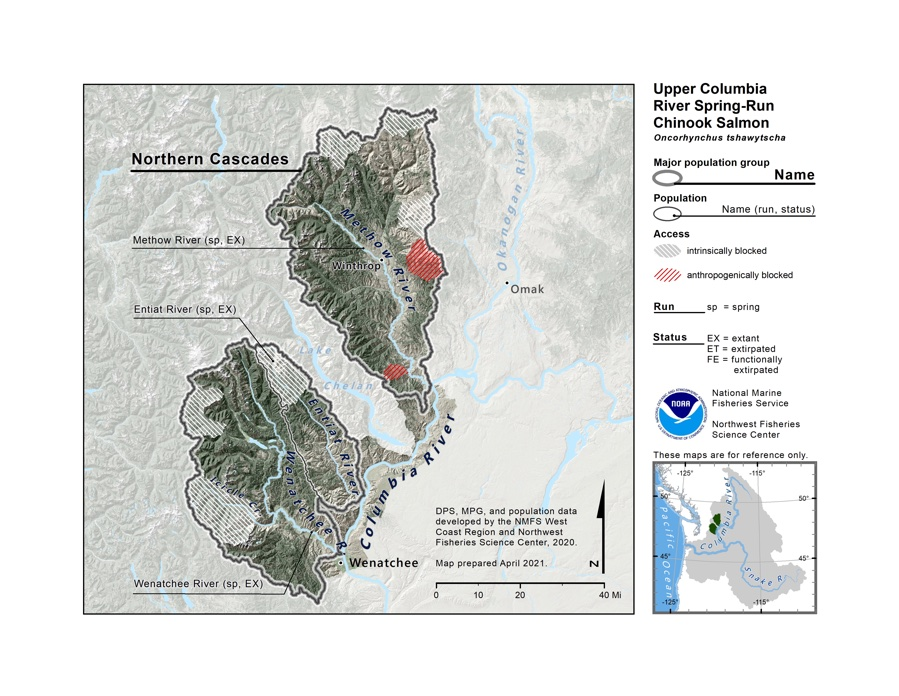
\includegraphics[width=3in,height=\textheight]{content/Interior_Columbia/../../media/image8.jpg}

}

\caption{\label{fig-UCR-Spr-Chinook-spawning-areas}Map of the Upper
Columbia River Chinook salmon ESU's spawning and rearing areas,
illustrating populations and major population groups.}

\end{figure}

\hypertarget{summary-of-previous-viability-conclusions-1}{%
\section{Summary of previous viability
conclusions}\label{summary-of-previous-viability-conclusions-1}}

\emph{2005}

In the 2005 review, a slight majority (53\%) of the cumulative votes
cast by the BRT members placed this ESU in the ``in danger of
extinction'' category, with the next category, ``likely to become
endangered'', receiving a substantial number of votes as well (45\%)
(Good \emph{et al.} 2005). The 2005 BRT review noted that Upper Columbia
Spring Chinook populations had ``rebounded somewhat from the critically
low levels'' observed in the 1998 review. Although the BRT considered
this an encouraging sign, they noted that the increase was largely
driven by returns in the two most recent spawning years available at the
time of the review. The BRT ratings were also influenced by the fact
that two out of the three extant populations in this ESU were subject to
extreme hatchery intervention measures in response to the extreme
downturn in returns during the 1990s. Good \emph{et al}. (2005) stated
that these measures were ``...a strong indication of the ongoing risks
to this ESU, although the associated hatchery programs may ultimately
play a role in helping to restore naturally self-sustaining
populations.''

\emph{2010 }

The viability of the ESU in 2010 was reported in Ford \emph{et al}.
(2011). At that time, the Upper Columbia Spring Chinook ESU was not
currently meeting the viability criteria (adapted from the ICTRT) in the
Upper Columbia Recovery Plan. Increases in natural origin abundance
relative to the extremely low spawning levels observed in the mid-1990s
were encouraging; however, average productivity levels remained
extremely low. Overall, the report concluded that the viability of the
Upper Columbia Spring Chinook salmon ESU had likely improved somewhat
since the time of the last BRT status review, but the ESU was still
clearly at moderate-to-high risk of extinction.

\emph{2015}

Estimates of natural origin spawner abundance increased relative to the
levels observed in the prior reviews for all three extant populations,
and productivities were higher for the Wenatchee and Entiat and
unchanged for the Methow (NWFSC 2015). However abundance and
productivity remained well below the viable thresholds called for in the
Upper Columbia Recovery Plan for all three populations. Based on the
information available for the 2015 review, the risk category for the
Upper Columbia Spring Chinook ESU remained unchanged from the prior
review. Although the viability of the ESU is improved relative to
measures available at the time of listing, all three populations remain
at high risk.

\hypertarget{description-of-new-data-available-for-this-review-1}{%
\section{Description of new data available for this
review}\label{description-of-new-data-available-for-this-review-1}}

Annual abundance estimates for each of the extant populations in this
ESU are generated based on expansions from redd surveys and carcass
sampling. Index area redd counts have been conducted in these river
systems since the late 1950's (Mullan \emph{et al.} 1992). Multiple pass
surveys in index areas complemented by supplemental surveys covering the
majority of spawning reaches have been conducted since the mid 1980's.
For more recent years, estimates of annual returns to the Wenatchee
River population also reflect counts and sampling data obtained at a
trap at the Tumwater Dam on the mainstem river downstream of spring
Chinook spawning areas. The data series for each population has been
updated to include return years through 2019. Recent year estimates of
spawner abundance, hatchery and natural origin proportions and age
composition were provided by the Washington Department of Fish and
Wildlife, recruits per spawner data for these populations was provided
by WDFW and distributed through the Coordinated Assessments data web
portal, and smolt to adult return rate data were estimated from PIT tag
detections and distributed by the Columbia River Data Access in Real
Time data portal{[}\^{}3{]}.

\emph{Smolt to Adult Return and Recruits per Spawner Rates}

Smolt to Adult Return (SAR) estimates (Bonneville to Bonneville) for all
three Upper Columbia River Spring Chinook salmon population data series
are generated by the Columbia River Data Access in Real Time (CBR \&
Washington 2020) project using PIT tag detections from all release
locations within each population basin (Columbia River DART \emph{et
al.} 2020). The indices represent cumulative marine, nearshore and
estuary survival. The SAR series includes estimates for the range of
brood years 2002-2015 (Figure 4). Over the period of record, the
geometric mean SAR for the Entiat and Methow populations
(\textasciitilde3\%) represents a low, but reasonable marine survival,
with the Wenatchee SAR of \textasciitilde1.5\% being on the low end, as
2\% is roughly a replacement rate. Recruits per Spawner (R/S) indices
are reported as available from the StreamNet Coordinated Assessments
data portal (see footnote). All populations in the ESU have low
(\textless{} 1.0) R/S values, implying that the natural replacement rate
is not keeping up with all sources of mortality across the life-cycle.

\begin{figure}

{\centering 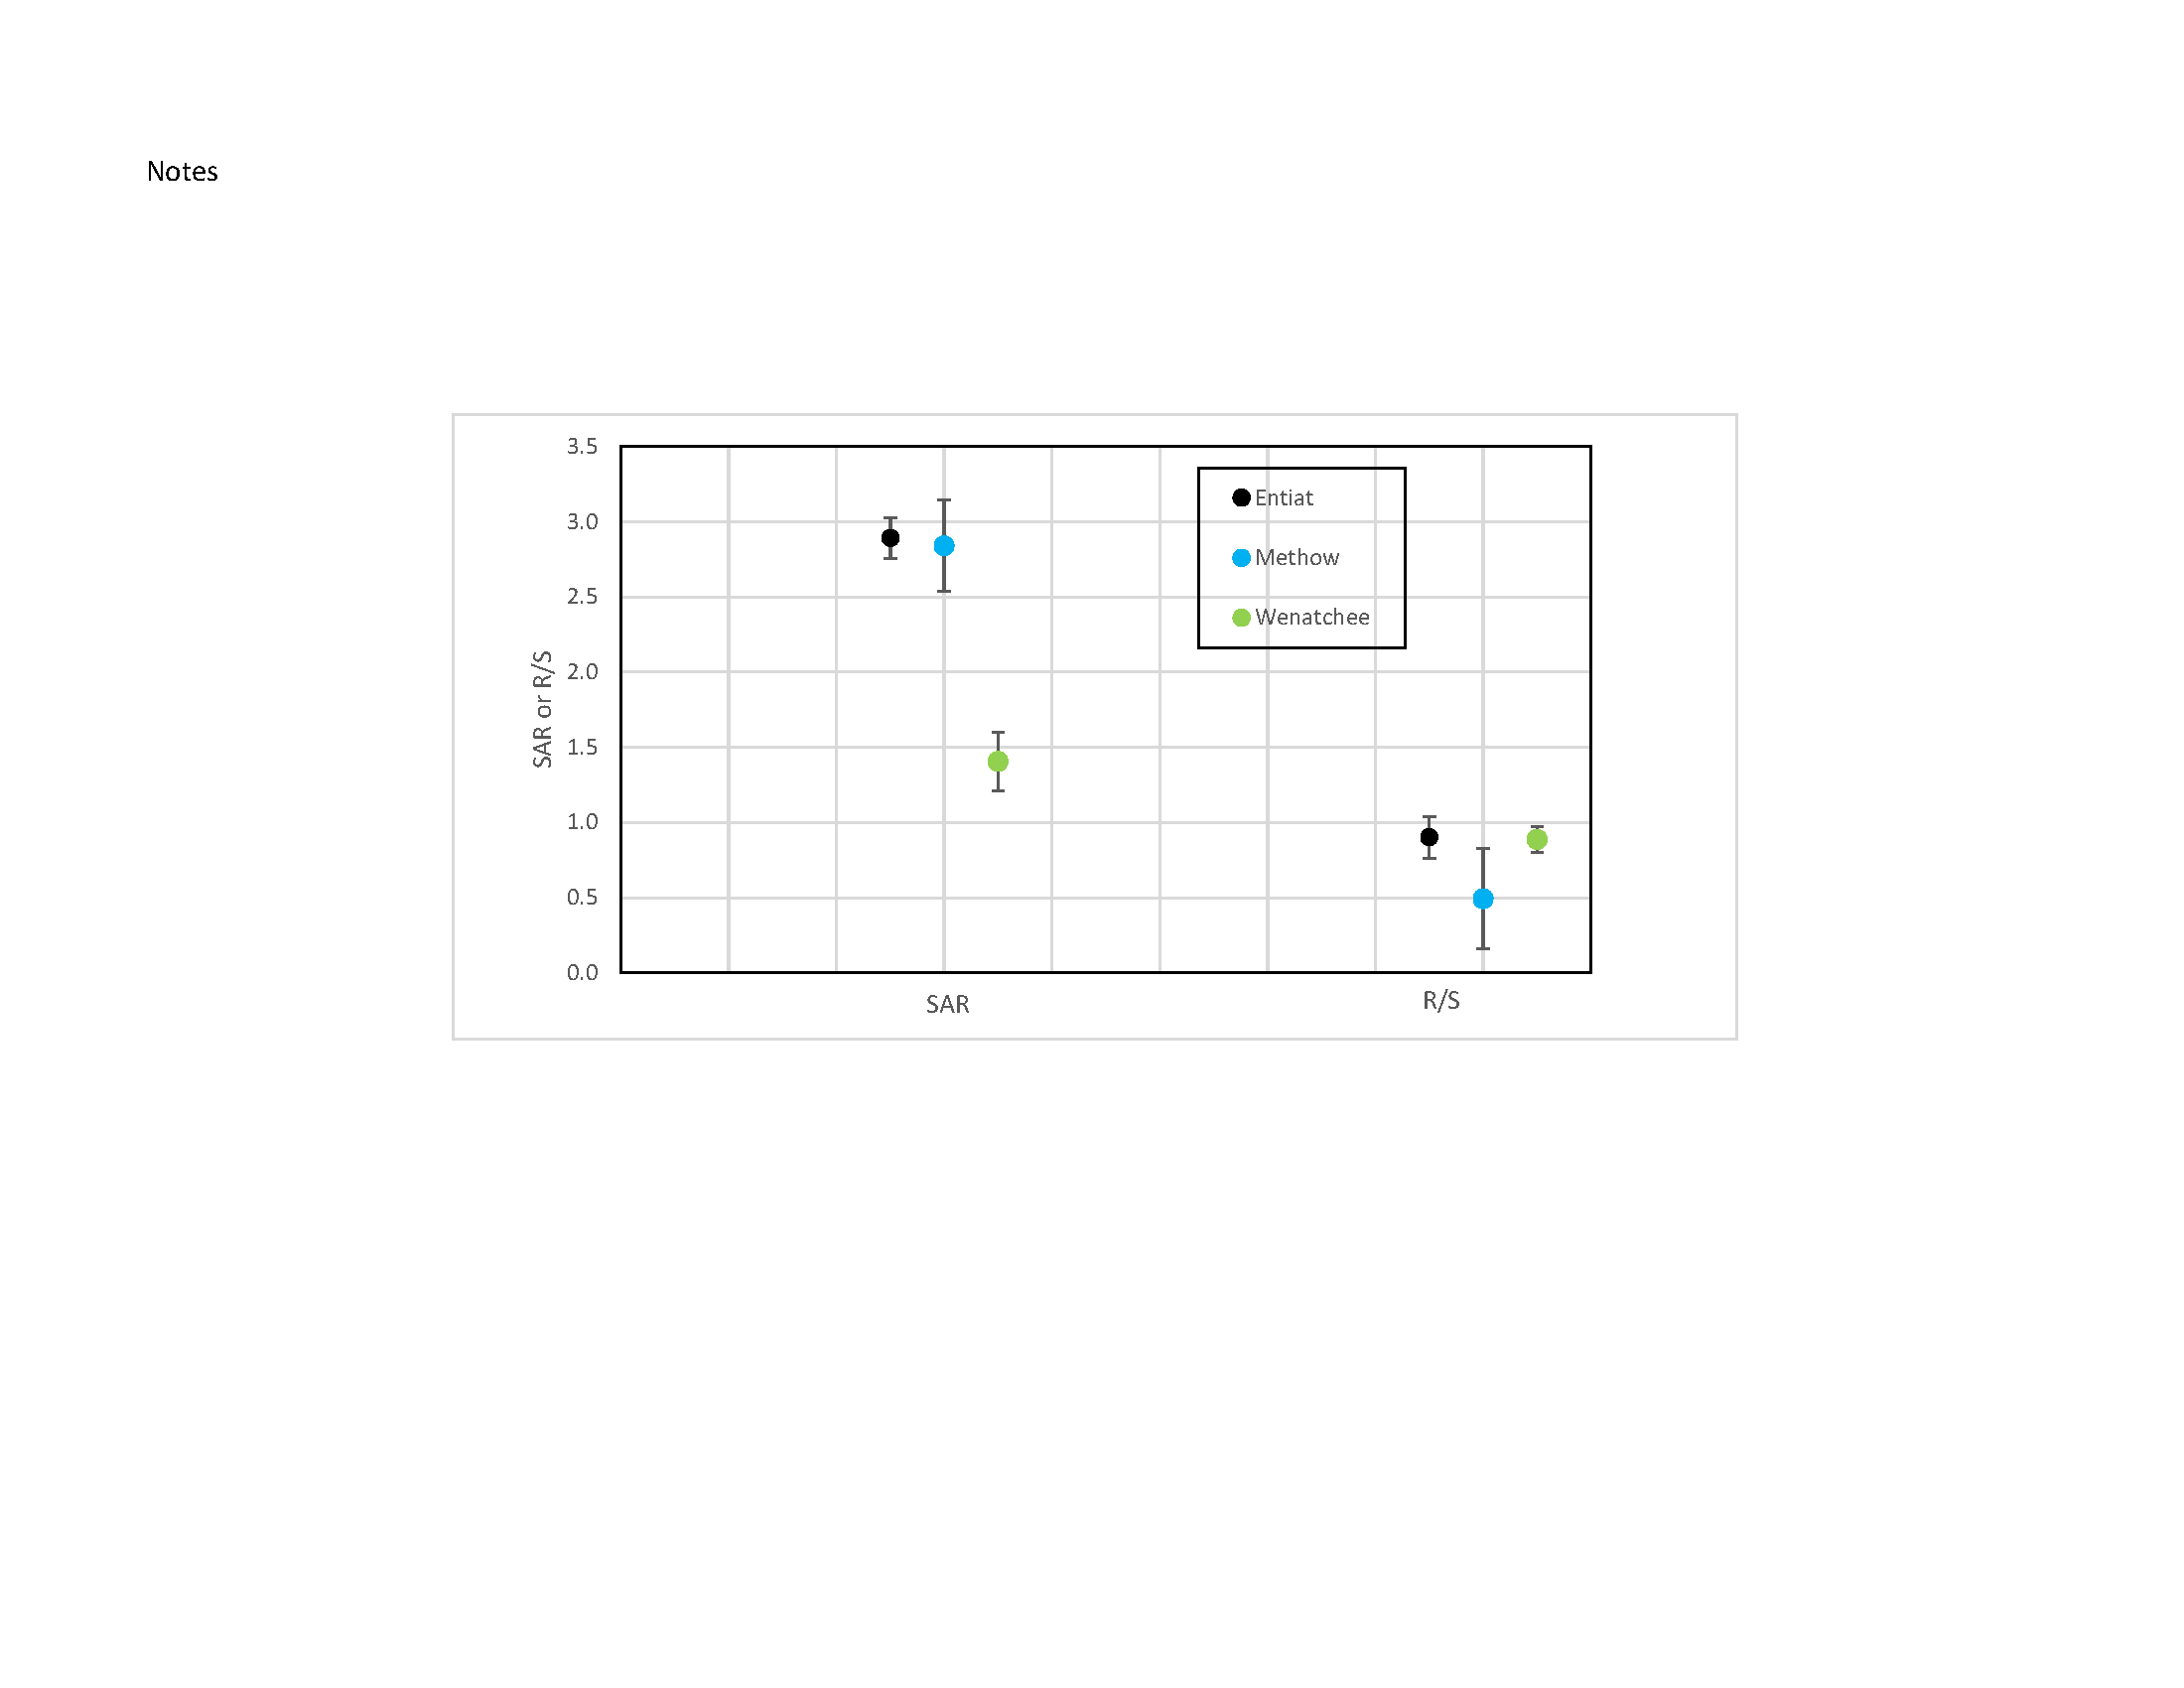
\includegraphics[width=4.65in,height=\textheight]{content/Interior_Columbia/../../media/image9.png}

}

\caption{\label{fig-UC-Spr-Chinook-Smolt-to-Adult}Smolt to Adult Return
and Recruits per Spawner for each of the populations in the ESU.
Geometric means of SAR (\%) and R/S (fish/fish) are shown for each
population, along with the standard error of the estimate (whiskers
represent +/- one standard error). The time period included in the SAR
or R/S indices is the past 20 years, depending on data availability.}

\end{figure}

\hypertarget{ocean-condition-indices}{%
\subsection{Ocean Condition Indices}\label{ocean-condition-indices}}

Upper Columbia spring Chinook salmon are a component of the Columbia
River spring Chinook run that is believed to occupy mid-shelf waters
during the early ocean life history phase. Aggregate annual returns of
Columbia River Spring Chinook are correlated with a range of ocean
condition indices including measures of broad scale physical conditions,
local biological indicators, and local physical factors (Peterson
\emph{et al.} 2014a). Several indicators, either individually or in
combination, correlate well with spring Chinook salmon adult returns
with a lag of 1 to 2 years. However, for each specific indicator or
combination, there are anomalous years that fall outside of the apparent
relationships. Work is continuing to further understand the
relationships among physical and biological `drivers' and annual levels
of ocean survival for salmonid species in the ocean environment. After
accounting for age at return at time of ocean entry, the annual pattern
in the Upper Columbia spring Chinook ESU SAR index generally corresponds
to the composite rankings across ocean indicators available for early
ocean years starting in the late 1990s (Peterson \emph{et al.} 2014b).
Indicators of ocean condition are highly correlated with each other, and
exhibit strong temporal autocorrelation (Figure 129) (Peterson \emph{et
al.} 2019). As a result, when indicators point to conditions that result
in poor ocean productivity for salmonid populations, they do so as a
suite of indicators, and for runs of `good' or `bad' years (see Habitat
chapter). Historically, ocean conditions cycled between periods of high
and low productivity. However, global climate change is likely to
disrupt this pattern, in general, leading to a preponderance of low
productivity years, with an unknown temporal distribution (Crozier
\emph{et al.} 2019b). Recent (2015-2019) ensemble ocean indicators
rankings include four of the worst seven years in the past 20, meaning
that an entire Chinook salmon generation has been subjected to poor
ocean productivity conditions (Figure 129).

\hypertarget{abundance-and-productivity-1}{%
\section{Abundance and
productivity}\label{abundance-and-productivity-1}}

Updated data series on spawner abundance, age structure and
hatchery/natural proportions were used to generate current assessments
of abundance and productivity at the population level. Evaluations were
done using both a set of metrics similar to those used in prior
Biological Review Team (BRT) reviews (see Methods) as well as a set
corresponding to the specific viability criteria based on ICTRT
recommendations for this ESU. The BRT level metrics were consistently
done across all ESUs and DPSs to facilitate comparisons across domains.
Assessments using the ICTRT metrics are described in the TRT and
Recovery Plan Criteria section below. The ICTRT abundance and
productivity metrics are measured over longer time frames to dampen the
effects of annual variations and they use annual natural origin age
composition to calculate brood year recruitment when sampling levels
meet regional fishery agency criteria.

Annual spawning escapements for all three of the extant Upper Columbia
spring Chinook populations showed steep declines beginning in the late
1980s, leading to extremely low abundance levels in the mid-1990s
(Figure 5, Table 2). The steep downward trend reflects the extremely low
return rates for natural production from the 1990-94 brood years (Figure
6). Estimated replacement rates were consistently below 1.0 even at low
parent spawner levels throughout the 1990s. Steeply declining trends
across indices of total spawner abundance were a major consideration in
the 1998 BRT risk assessment prior to listing of the ESU. Using the
updated data series for this review, the short-term (5 year) trend in
wild spawners has been strongly negative for all three extant
populations (Table 2). Longer term (15 year) trends are also negative
for all three populations, although the 95\% confidence intervals in
each case include 0 (Table 3). In general, both total and natural origin
escapements for all three populations increased sharply from 1999
through 2002 and have shown substantial year to year variations in the
years following, with peaks around 2001 and 2010 and declines after
2010. Average natural origin returns remain well below ICTRT minimum
threshold levels.

\begin{figure}

{\centering 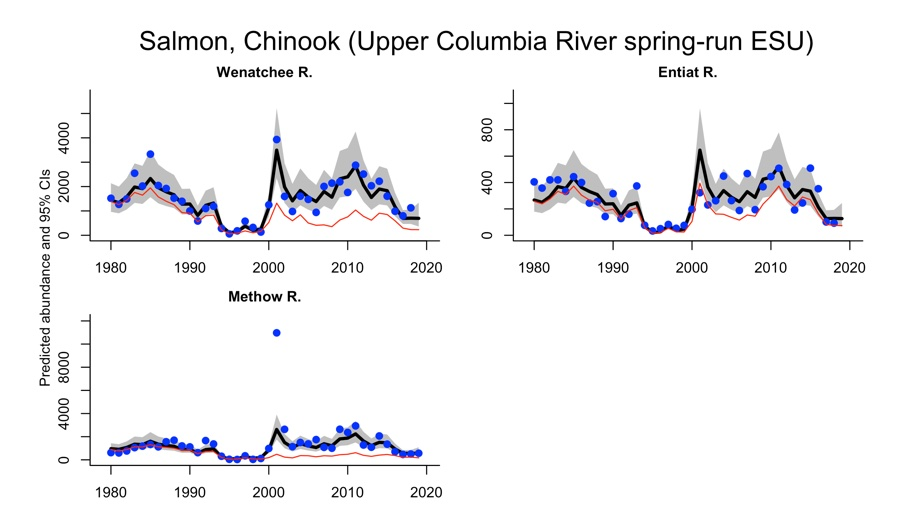
\includegraphics[width=3in,height=\textheight]{content/Interior_Columbia/../../media/image10.jpg}

}

\caption{\label{fig-UC-Spr-Chinook-smoothed-trends}Smoothed trend in
estimated total (thick black line, with 95\% confidence internal in
gray) and natural (thin red line) population spawning abundance. In
portions of a time series where a population has no annual estimates but
smoothed spawning abundance is estimated from correlations with other
populations the smoothed estimate is shown in light gray. Points show
the annual raw spawning abundance estimates. For some trends the
smoothed estimate may be influenced by earlier data points not included
in the plot.}

\end{figure}

The annual natural return per spawner series for each population
directly reflects the patterns in natural origin abundance and was only
positive during a period of strong population increase Figure 6). Brood
year escapements with positive return per spawner values are associated
with those years leading up to the peaks in natural origin spawner
returns in each series. Using the R/S and SAR indicators by population
(Figure 4), it is possible to generate an indicator of fresh water
productivity (FWPI) as a ratio of R/S and SAR. This quantity can be
thought of as an indicator of smolts per spawner, and thus, the overall
population productivity in the freshwater environment. FWPI for Upper
Columbia Spring Chinook populations are low (\textless100, Figure 7),
confirming areas of recovery action focus such as pre-spawn mortality
and juvenile rearing habitat condition. The initial risk assessment for
this ESU (ICTRT 2007) found that achieving natural origin abundance and
productivity levels above the threshold viability curve corresponding to
5\% risk in extinction will require substantial improvements in survival
and/or natural production capacity. The long-term population
productivity data indicates that this assessment is still valid.

\begin{figure}

{\centering 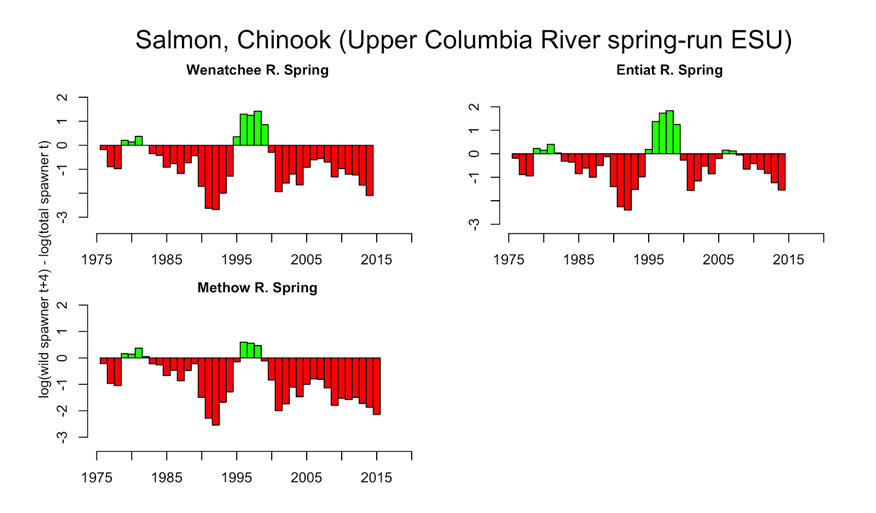
\includegraphics[width=2.92in,height=\textheight]{content/Interior_Columbia/../../media/image11.png}

}

\caption{\label{fig-UC-Spr-Chinook-productivity-trends}Trends in
population productivity, estimated as the log of the smoothed natural
spawning abundance in year \emph{t} divided by the smoothed natural
spawning abundance in year \emph{t}- 4. Spawning years on x axis.}

\end{figure}

\begin{figure}

{\centering 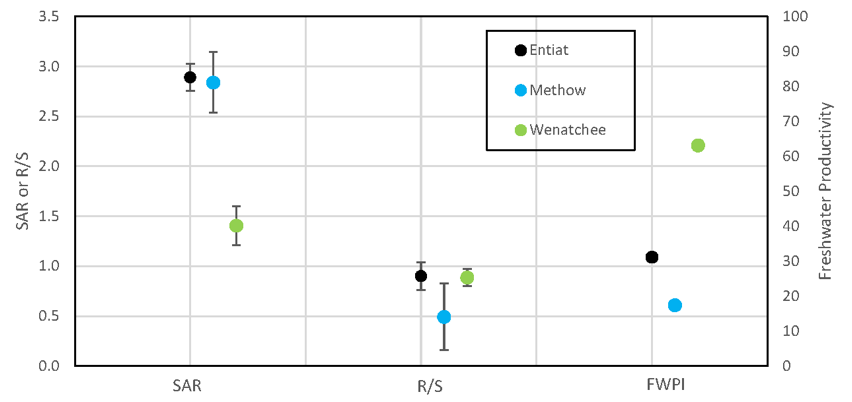
\includegraphics[width=2.84in,height=\textheight]{content/Interior_Columbia/../../media/image12.png}

}

\caption{\label{fig-UC-Spr-Chinook-Smolt-to-Adult-Productivity}Smolt to
Adult Return, Recruits per Spawner, and Freshwater Productivity Index
(FWPI) for each of the populations in the ESU. Geometric means of SAR
and R/S are shown for each population, along with the standard error of
the estimate (whiskers represent +/- one standard error). The time
period included in the SAR or R/S indices is the past 20 years,
depending on data.}

\end{figure}

\begin{longtable}[]{@{}
  >{\raggedleft\arraybackslash}p{(\columnwidth - 16\tabcolsep) * \real{0.1238}}
  >{\centering\arraybackslash}p{(\columnwidth - 16\tabcolsep) * \real{0.1048}}
  >{\raggedleft\arraybackslash}p{(\columnwidth - 16\tabcolsep) * \real{0.1143}}
  >{\raggedleft\arraybackslash}p{(\columnwidth - 16\tabcolsep) * \real{0.1143}}
  >{\raggedleft\arraybackslash}p{(\columnwidth - 16\tabcolsep) * \real{0.1143}}
  >{\raggedleft\arraybackslash}p{(\columnwidth - 16\tabcolsep) * \real{0.1143}}
  >{\raggedleft\arraybackslash}p{(\columnwidth - 16\tabcolsep) * \real{0.1143}}
  >{\raggedleft\arraybackslash}p{(\columnwidth - 16\tabcolsep) * \real{0.1143}}
  >{\centering\arraybackslash}p{(\columnwidth - 16\tabcolsep) * \real{0.0857}}@{}}
\caption{Table . 5-year mean of fraction natural origin (sum of all
estimates divided by the number of estimates). Blanks mean no estimate
available in that 5-year range.}\tabularnewline
\toprule()
\begin{minipage}[b]{\linewidth}\raggedleft
Population
\end{minipage} & \begin{minipage}[b]{\linewidth}\centering
MPG
\end{minipage} & \begin{minipage}[b]{\linewidth}\raggedleft
1990-1994
\end{minipage} & \begin{minipage}[b]{\linewidth}\raggedleft
1995-1999
\end{minipage} & \begin{minipage}[b]{\linewidth}\raggedleft
2000-2004
\end{minipage} & \begin{minipage}[b]{\linewidth}\raggedleft
2005-2009
\end{minipage} & \begin{minipage}[b]{\linewidth}\raggedleft
2010-2014
\end{minipage} & \begin{minipage}[b]{\linewidth}\raggedleft
2015-2019
\end{minipage} & \begin{minipage}[b]{\linewidth}\centering
\% Change
\end{minipage} \\
\midrule()
\endfirsthead
\toprule()
\begin{minipage}[b]{\linewidth}\raggedleft
Population
\end{minipage} & \begin{minipage}[b]{\linewidth}\centering
MPG
\end{minipage} & \begin{minipage}[b]{\linewidth}\raggedleft
1990-1994
\end{minipage} & \begin{minipage}[b]{\linewidth}\raggedleft
1995-1999
\end{minipage} & \begin{minipage}[b]{\linewidth}\raggedleft
2000-2004
\end{minipage} & \begin{minipage}[b]{\linewidth}\raggedleft
2005-2009
\end{minipage} & \begin{minipage}[b]{\linewidth}\raggedleft
2010-2014
\end{minipage} & \begin{minipage}[b]{\linewidth}\raggedleft
2015-2019
\end{minipage} & \begin{minipage}[b]{\linewidth}\centering
\% Change
\end{minipage} \\
\midrule()
\endhead
Wenatchee R Spring & . North Cascades & 380 (735) & 99 (192) & 668
(1652) & 379 (1671) & 874 (2247) & 443 (1092) & -49 (-51) \\
Entiat R. Spring & North Cascades & 153 (179) & 37 (56) & 148 (280) &
129 (278) & 256 (333) & 137 (202) & -46 (-39) \\
Methow R. Spring & North Cascades & 726 (867) & 44 (75) & 292 (2171) &
379 (1470) & 448 (1820) & 232 (659) & -48 (-64) \\
\bottomrule()
\end{longtable}

\begin{longtable}[]{@{}
  >{\raggedright\arraybackslash}p{(\columnwidth - 6\tabcolsep) * \real{0.2800}}
  >{\raggedright\arraybackslash}p{(\columnwidth - 6\tabcolsep) * \real{0.2133}}
  >{\raggedright\arraybackslash}p{(\columnwidth - 6\tabcolsep) * \real{0.2400}}
  >{\raggedright\arraybackslash}p{(\columnwidth - 6\tabcolsep) * \real{0.2400}}@{}}
\caption{Table . Upper Columbia spring Chinook salmon ESU population
viability status summary. Current abundance and productivity estimates
are geometric means (most recent 10 years for abundance and 20 years for
productivity). Standard deviation of annual abundance, standard error
and number of qualifying estimates for productivities in
parentheses.}\tabularnewline
\toprule()
\begin{minipage}[b]{\linewidth}\raggedright
Population
\end{minipage} & \begin{minipage}[b]{\linewidth}\raggedright
MPG
\end{minipage} & \begin{minipage}[b]{\linewidth}\raggedright
1990-2005
\end{minipage} & \begin{minipage}[b]{\linewidth}\raggedright
2004-2019
\end{minipage} \\
\midrule()
\endfirsthead
\toprule()
\begin{minipage}[b]{\linewidth}\raggedright
Population
\end{minipage} & \begin{minipage}[b]{\linewidth}\raggedright
MPG
\end{minipage} & \begin{minipage}[b]{\linewidth}\raggedright
1990-2005
\end{minipage} & \begin{minipage}[b]{\linewidth}\raggedright
2004-2019
\end{minipage} \\
\midrule()
\endhead
Wenatchee R. Spring & North Cascades & 0.03 (-0.09, 0.14) & -0.03
(-0.09, 0.02) \\
Entiat R. Spring & North Cascades & 0.03 (-0.09, 0.15) & -0.03 (-0.09,
0.03) \\
Methow R. Spring & North Cascades & -0.05 (-0.15, 0.06) & -0.03 (-0.06,
0.01) \\
\bottomrule()
\end{longtable}

\hypertarget{non-treaty-harvest-1}{%
\subsection{Non-treaty Harvest}\label{non-treaty-harvest-1}}

Spring Chinook salmon from the upper Columbia basin migrate offshore in
marine water and where impacts in ocean salmon fisheries are too low to
be quantified. The only significant harvest in salmon fisheries occurs
in the mainstem Columbia River in tribal and non-tribal fisheries
directed at hatchery spring Chinook salmon from the Columbia and
Willamette Rivers. Exploitation rates have remained relatively low,
generally below the target rate of 2\% (Figure 8).

Figure . Non-treaty harvest rate for upper Columbia River spring Chinook
salmon. Data from the Columbia River Technical Advisory Committee (TAC
(U.S. v Oregon Technical Advisory Committee) 2020).

\hypertarget{spatial-structure-and-diversity-1}{%
\section{Spatial structure and
diversity}\label{spatial-structure-and-diversity-1}}

The proportions of natural origin contributions to spawning in the
Wenatchee and Methow populations have trended downwards from 1990 to
2008 (Figure 9, Table 4), reflecting the large increase in releases and
subsequent returns from the directed supplementation programs in those
two drainages (Hillman \emph{et al.} 2015). Natural origin fractions
increased from 2009 to 2017, reflecting increasing natural origin
abundance trends and changes to hatchery management, before declining
again in the two years. There is currently no direct spring run hatchery
supplementation program in the Entiat River, though the summer run
releases do have the potential to impact the spring run through redd
superimposition. Prior to 2011, hatchery-origin spawners in the Entiat
River system are predominately strays from Entiat NFH releases. The
Entiat NFH spring Chinook release program was discontinued in 2007, and
the upward trend in proportional natural origin since then can be
attributed to that closure. In recent years, hatchery supplementation
returns from the adjacent Wenatchee River program have also strayed into
the Entiat (Ford \emph{et al.} 2015). The nearby Eastbank Hatchery
facility is used for rearing the Wenatchee River supplementation stock
prior to transfer to the Chiwawa acclimation pond. It is possible that
some of the returns from that program are homing on the Eastbank
facility and then straying into the Entiat River, the nearest spawning
area.

\begin{figure}

{\centering 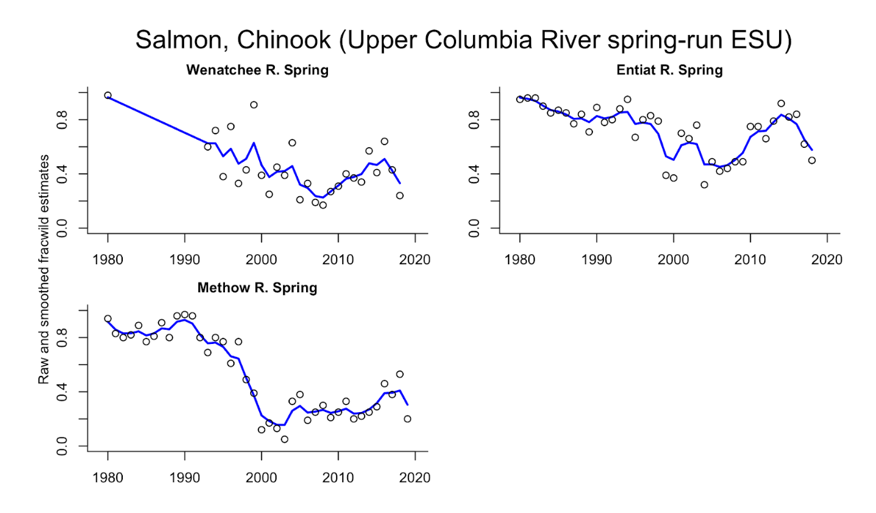
\includegraphics[width=2.92in,height=\textheight]{content/Interior_Columbia/../../media/image13.png}

}

\caption{\label{fig-UC-Spr-Chinook-smoothed-frac-wild}Smoothed trend in
the estimated fraction of the natural spawning population consisting of
fish if natural origin. Points show the annual raw estimates.}

\end{figure}

\begin{longtable}[]{@{}
  >{\raggedright\arraybackslash}p{(\columnwidth - 10\tabcolsep) * \real{0.2346}}
  >{\raggedright\arraybackslash}p{(\columnwidth - 10\tabcolsep) * \real{0.1481}}
  >{\raggedright\arraybackslash}p{(\columnwidth - 10\tabcolsep) * \real{0.1481}}
  >{\raggedright\arraybackslash}p{(\columnwidth - 10\tabcolsep) * \real{0.1481}}
  >{\raggedright\arraybackslash}p{(\columnwidth - 10\tabcolsep) * \real{0.1481}}
  >{\raggedright\arraybackslash}p{(\columnwidth - 10\tabcolsep) * \real{0.1481}}@{}}
\caption{Table . 5-year geometric mean of raw natural spawner counts.
This is the raw total spawner count times the fraction natural estimate,
if available. In parentheses, 5-year geometric mean of raw total spawner
counts is shown. A value only in parentheses means that a total spawner
count was available but no or only one estimate of natural spawners
available. The geometric mean was computed as the product of counts
raised to the power 1 over the number of counts available (2 to 5). A
minimum of 2 values was used to compute the geometric mean. Percent
change between the most recent two 5-year periods is shown on the far
right.}\tabularnewline
\toprule()
\begin{minipage}[b]{\linewidth}\raggedright
Population
\end{minipage} & \begin{minipage}[b]{\linewidth}\raggedright
1995-1999
\end{minipage} & \begin{minipage}[b]{\linewidth}\raggedright
2000-2004
\end{minipage} & \begin{minipage}[b]{\linewidth}\raggedright
2005-2009
\end{minipage} & \begin{minipage}[b]{\linewidth}\raggedright
2010-2014
\end{minipage} & \begin{minipage}[b]{\linewidth}\raggedright
2015-2019
\end{minipage} \\
\midrule()
\endfirsthead
\toprule()
\begin{minipage}[b]{\linewidth}\raggedright
Population
\end{minipage} & \begin{minipage}[b]{\linewidth}\raggedright
1995-1999
\end{minipage} & \begin{minipage}[b]{\linewidth}\raggedright
2000-2004
\end{minipage} & \begin{minipage}[b]{\linewidth}\raggedright
2005-2009
\end{minipage} & \begin{minipage}[b]{\linewidth}\raggedright
2010-2014
\end{minipage} & \begin{minipage}[b]{\linewidth}\raggedright
2015-2019
\end{minipage} \\
\midrule()
\endhead
Wenatchee R. Spring & 0.56 & 0.42 & 0.23 & 0.40 & 0.43 \\
Entiat R. Spring & 0.70 & 0.56 & 0.47 & 0.77 & 0.70 \\
Methow R. Spring & 0.61 & 0.16 & 0.27 & 0.25 & 0.37 \\
\bottomrule()
\end{longtable}

\hypertarget{biological-viability-relative-to-recovery-goals-1}{%
\section{Biological viability relative to recovery
goals}\label{biological-viability-relative-to-recovery-goals-1}}

NOAA Fisheries (National Marine Fisheries Service adopted a recovery
plan for Upper Columbia Spring Chinook and steelhead in 2007 (FR 72
\#194. 57303-57307). The Plan was developed by the Upper Columbia Salmon
Recovery Board (UCSRB) and is available through their website
(http://www.ucsrb.com/). The Upper Columbia Salmon Recovery Plan's
overall goal is ``...to achieve recovery and delisting of spring Chinook
salmon and steelhead by ensuring the long-term persistence of viable
populations of naturally produced fish distributed across their native
range.''

Two incremental levels of recovery objectives are incorporated into the
Upper Columbia Salmon Recovery Plan. Increasing natural production
sufficiently to upgrade each Upper Columbia River ESU from
``endangered'' to ``threatened'' status is stated as an initial
objective. The Plan includes three specific quantitative
reclassification criteria expressed relative to population viability
curves (ICTRT 2007a). Abundance and productivity of natural origin
spring Chinook salmon within each of the extant Upper Columbia
populations, measured as 8-year geometric means (representing
approximately two generations), must fall above the viability curve
representing the minimum combinations projecting to a 10\% risk of
extinction over 100 years. In addition, the plan incorporates explicit
criteria for spatial structure and diversity adopted from the ICTRT
viability report. The mean score for the three metrics representing
natural rates and spatially mediated processes should result in a
moderate or lower risk in each of the three populations and all threats
defined as high risk must be addressed. In addition, the mean score for
the eight ICTRT metrics tracking natural levels of variation should
result in a moderate or lower risk score at the population level.

Achieving recovery (delisting) of each ESU via sufficient improvement in
the abundance, productivity, spatial structure and diversity is the
longer-term goal of the UCSRB Plan. The Plan includes two specific
quantitative criteria for assessing the status of the Spring Chinook ESU
against the recovery objective; ``The 12-year geometric mean
(representing approximately three generations) of abundance and
productivity of naturally produced spring Chinook within the Wenatchee,
Entiat and Methow populations must reach a level that would have not
less than a 5\% extinction-risk (viability) over a 100 year period'' and
``at a minimum, the Upper Columbia Spring Chinook ESU will maintain at
least 4,500 naturally produced spawners and a spawner:spawner ratio
greater than 1:1 distributed among the three populations''. The minimum
number of naturally produced spawners (expressed as 12 year geometric
means) should exceed 2,000 each for the Wenatchee and Methow River
populations and 500 within the Entiat River. Minimum productivity
thresholds were also established in the Plan. The 12-year geometric mean
productivity should exceed 1.2 spawners per parent spawner for the two
larger populations (Wenatchee and Methow Rivers), and 1.4 for the
smaller Entiat River population. The ICTRT had recommended that at least
two of the three extant populations be targeted for highly viable status
(less than 1\% risk of extinction over 100 years) because of the
relatively low number of extant populations remaining in the ESU. The UC
Plan adopted an alternative approach for addressing the limited number
of populations in the ESU -- 5\% or less risk of extinction for all
three extant populations.

The Upper Columbia Salmon Recovery Plan also calls for '\ldots{}
restoring the distribution of naturally produced spring Chinook salmon
and steelhead to previously occupied areas where practical; and
conserving their genetic and phenotypic diversity.'' Specific criteria
included in the UCSRB Plan reflect a combination of the specific
criteria recommended by the ICTRT (ICTRT 2007) and in the earlier QAR
effort (Ford \emph{et al.} 2001). The Plan incorporates spatial
structure criteria specific to each spring Chinook salmon population.
For the Wenatchee River population, the criteria call for observed
natural spawning in four of the five major spawning areas as well as in
at least one of the minor spawning areas downstream of Tumwater Dam. In
the Methow River, natural spawning should be observed in three major
spawning areas. In each case, the major spawning areas should include a
minimum of 5\% of the total return to the system or 20 redds, whichever
is greater. The Entiat River Spring Chinook population includes a single
historical major spawning area.

\begin{longtable}[]{@{}
  >{\raggedright\arraybackslash}p{(\columnwidth - 16\tabcolsep) * \real{0.1486}}
  >{\raggedright\arraybackslash}p{(\columnwidth - 16\tabcolsep) * \real{0.0946}}
  >{\raggedright\arraybackslash}p{(\columnwidth - 16\tabcolsep) * \real{0.0946}}
  >{\raggedright\arraybackslash}p{(\columnwidth - 16\tabcolsep) * \real{0.1081}}
  >{\raggedright\arraybackslash}p{(\columnwidth - 16\tabcolsep) * \real{0.0946}}
  >{\raggedright\arraybackslash}p{(\columnwidth - 16\tabcolsep) * \real{0.0946}}
  >{\raggedright\arraybackslash}p{(\columnwidth - 16\tabcolsep) * \real{0.0811}}
  >{\raggedright\arraybackslash}p{(\columnwidth - 16\tabcolsep) * \real{0.1081}}
  >{\raggedright\arraybackslash}p{(\columnwidth - 16\tabcolsep) * \real{0.0811}}@{}}
\caption{Table . 15-year trends in log wild spawner abundance computed
from a linear regression applied to the smoothed wild spawner log
abundance estimate. Only populations with at least 4 wild spawner
estimates from 1980 to 2014 are shown and with at least 2 data points in
the first 5 years and last 5 years of the 15-year
period.}\tabularnewline
\toprule()
\begin{minipage}[b]{\linewidth}\raggedright
Po pulation
\end{minipage} & \begin{minipage}[b]{\linewidth}\raggedright
Ab unda nce/ Prod ucti vity Met rics
\end{minipage} & \begin{minipage}[b]{\linewidth}\raggedright
\end{minipage} & \begin{minipage}[b]{\linewidth}\raggedright
\end{minipage} & \begin{minipage}[b]{\linewidth}\raggedright
\end{minipage} & \begin{minipage}[b]{\linewidth}\raggedright
Spa tial S truc ture and D iver sity Met rics
\end{minipage} & \begin{minipage}[b]{\linewidth}\raggedright
\end{minipage} & \begin{minipage}[b]{\linewidth}\raggedright
\end{minipage} & \begin{minipage}[b]{\linewidth}\raggedright
O ver all R isk Rat ing
\end{minipage} \\
\midrule()
\endfirsthead
\toprule()
\begin{minipage}[b]{\linewidth}\raggedright
Po pulation
\end{minipage} & \begin{minipage}[b]{\linewidth}\raggedright
Ab unda nce/ Prod ucti vity Met rics
\end{minipage} & \begin{minipage}[b]{\linewidth}\raggedright
\end{minipage} & \begin{minipage}[b]{\linewidth}\raggedright
\end{minipage} & \begin{minipage}[b]{\linewidth}\raggedright
\end{minipage} & \begin{minipage}[b]{\linewidth}\raggedright
Spa tial S truc ture and D iver sity Met rics
\end{minipage} & \begin{minipage}[b]{\linewidth}\raggedright
\end{minipage} & \begin{minipage}[b]{\linewidth}\raggedright
\end{minipage} & \begin{minipage}[b]{\linewidth}\raggedright
O ver all R isk Rat ing
\end{minipage} \\
\midrule()
\endhead
& \emph{I CTRT Th resh old} & \emph{Nat ural S pawn ing} &
\begin{minipage}[t]{\linewidth}\raggedright
\begin{itemize}
\tightlist
\item
  ICTRT Pro ducti vity*
\end{itemize}
\end{minipage} & \emph{In tegr ated A/P R isk} & \emph{Nat ural Pr oces
ses} & \begin{minipage}[t]{\linewidth}\raggedright
\begin{itemize}
\tightlist
\item
  Div ers ity Ri sk*
\end{itemize}
\end{minipage} & \begin{minipage}[t]{\linewidth}\raggedright
\begin{itemize}
\tightlist
\item
  Integ rated SS/D Risk*
\end{itemize}
\end{minipage} & \\
W enatchee River & 2 ,000 & 630

(sd. 261) & 0.89

( 0.09, 1 7/20) & High & Low & H igh & High & H igh \\
Entiat River & 500 & 193

(sd. 126) & 0.90

( 0.14, 1 9/20) & High & Mode rate & H igh & High & H igh \\
Methow River & 2 ,000 & 323

(sd. 251) & 0.49

( 0.33, 1 9/20) & High & Low & H igh & High & H igh \\
\bottomrule()
\end{longtable}

\hypertarget{recovery-update}{%
\section{Recovery Update}\label{recovery-update}}

The UCSRB Plan calls for meeting or exceeding the same basic spatial
structure and diversity criteria adopted from the ICTRT viability report
for recovery.

Overall abundance and productivity (A/P) remains rated at high risk for
the each of the three extant populations in this MPG/ESU (Table 5). The
10-year geometric mean abundance of adult natural-origin spawners has
not changed by more than 25\% relative to the levels reported in the
2015 status update. Natural origin escapements still remains well below
the corresponding ICTRT thresholds for all populations. The combinations
of current abundance and productivity for each population result in a
high risk rating when compared to the ICTRT viability curves.

The composite spatial structure/diversity (SS/D) risks for all three of
the extant populations in this MPG are rated at high (Table 5). The
spatial processes component of the SS/D risk is low for the Wenatchee
and Methow river populations and moderate for the Entiat River (due to a
loss of production in lower section which increases effective distance
to other populations). All three of the extant populations in this MPG
are rated at high risk for diversity, driven primarily by chronically
high proportions of hatchery-origin spawners in natural spawning areas
and lack of genetic diversity among the natural-origin spawners (ICTRT
2007).

Based on the combined ratings for A/P and SS/D, all three of the extant
populations of Upper Columbia spring Chinook salmon remain rated at high
overall risk (Table 5).

\hypertarget{updated-biological-risk-summary-1}{%
\section{Updated biological risk
summary}\label{updated-biological-risk-summary-1}}

Current estimates of natural origin spawner abundance decreased
substantially relative to the levels observed in the prior review for
all three extant populations. Productivities also continued to be very
low and both abundance and productivity remained well below the viable
thresholds called for in the Upper Columbia Recovery Plan for all three
populations. Short-term patterns in those indicators appear to be
largely driven by year-to year fluctuations in survival rates in areas
outside of these watersheds, in particular a recent run of poor ocean
condition years. All three populations continued to be rated at low risk
for spatial structure but at high risk for diversity criteria.
Large-scale supplementation efforts in the Methow and Wenatchee Rivers
are ongoing, intended to counter short-term demographic risks given
current average survival levels and the associated year-to-year
variability. Under the current recovery plan, habitat protection and
restoration actions are being implemented that are directed at key
limiting factors.

Given the high degree of year-to-year variability in life stage
survivals and the time lags resulting from the 5-year life cycle of the
populations, it is not possible to detect incremental gains from habitat
actions implemented to date in population level measures of adult
abundance or productivity. Efforts are underway to develop life stage
specific estimates of performance (survival and capacities) and to use a
life cycle model framework to evaluate progress (Zabel \& Jordan 2020,
chapter 6). Based on the information available for this review, the risk
category for the Upper Columbia Spring Chinook ESU remains unchanged
from the prior review (NWFSC 2015). Although the viability of the ESU
remains improved relative to measures available at the time of listing,
all three populations remain at high risk.

\bookmarksetup{startatroot}

\hypertarget{snake-river-springsummer-run-chinook-salmon-esu}{%
\chapter{Snake River Spring/summer-Run Chinook salmon
ESU}\label{snake-river-springsummer-run-chinook-salmon-esu}}

The Snake River Spring-Summer Chinook salmon ESU includes all naturally
spawned populations of spring/summer-run Chinook salmon in the mainstem
Snake River and the Tucannon River, Grande Ronde River, Imnaha River,
and Salmon River subbasins, as well as fifteen artificial propagation
programs (85 FR 81822, Figure~\ref{fig-SnR-SS-spawning-areas}). The ESU
was first listed under the ESA in 1992, and the listing was reaffirmed
in 2005 and 2012.

\begin{figure}

{\centering 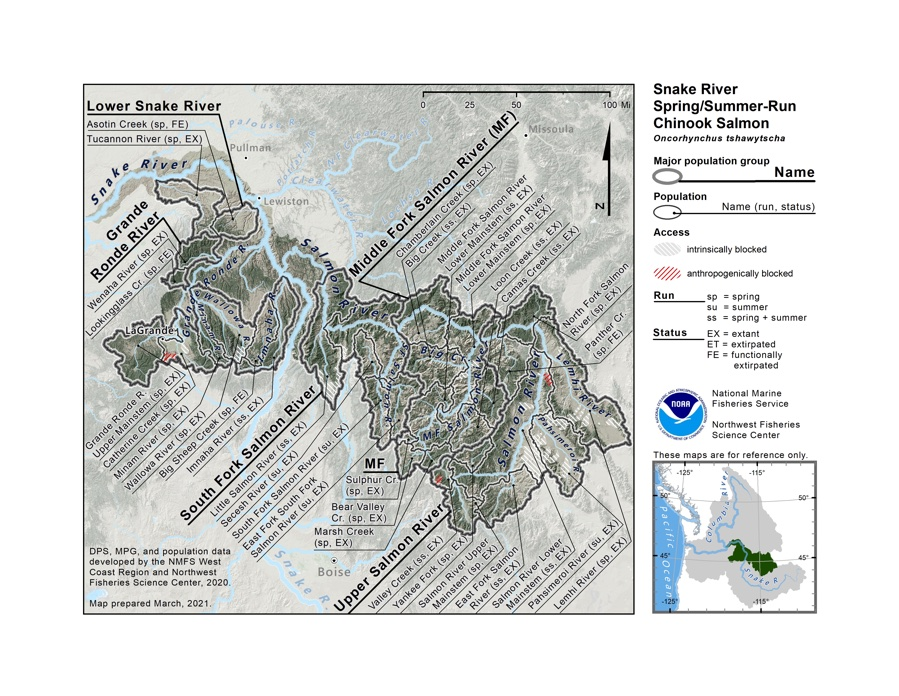
\includegraphics[width=3in,height=\textheight]{content/Interior_Columbia/../../media/image22.jpg}

}

\caption{\label{fig-SnR-SS-spawning-areas}The Snake River
spring/summer-run Chinook salmon ESU spawning and rearing areas,
illustrating populations and major population groups.}

\end{figure}

\hypertarget{summary-of-previous-viability-conclusions-2}{%
\section{Summary of previous viability
conclusions}\label{summary-of-previous-viability-conclusions-2}}

\emph{2005}

The 2005 BRT report evaluated the viability of Snake River spring/summer
Chinook using data on returns through 2001, with the majority of BRT
risk rating points being assigned to the most likely to be endangered
category (Good et al. 2005). The BRT noted that although there were a
number of extant spawning aggregations within this ESU, a substantial
number of historical spawning populations have been lost. The most
serious risk factor for the ESU was low natural productivity (spawner to
spawner return rates) and the associated decline in abundance to
extremely low levels relative to historical returns. Large increases in
escapement estimates for many (but not all) areas for the 2001 return
year were considered encouraging by the BRT. However the BRT also
acknowledged that return levels were highly variable and that abundance
should be measured over at least an 8 year period and that by this
measure the then recent abundance levels across the ESU fall short of
interim objectives. The BRT was concerned about the high level of
production/mitigation and supplementation hatchery programs across the
ESU, noting that these programs represented ongoing risks to natural
populations and made it difficult to assess trends in natural
productivity and growth rates. The phasing out of the non-native Rapid
River-origin hatchery program in the Grande Ronde Basin was viewed as a
positive action.

\emph{2010}

Ford et al. (2011) concluded that population level viability ratings
remained at high risk across all MPGs within the ESU; although natural
spawning abundance estimates had increased, all populations remained
below minimum natural origin abundance thresholds. Relatively low
natural production rates and spawning levels below minimum abundance
thresholds remained a major concern across the ESU. The ability of
populations to be self-sustaining through normal periods of relatively
low ocean survival remained uncertain. Factors cited by the 2005 BRT
(Good et al. 2005) remained as concerns or key uncertainties for several
populations. Overall, the new information considered in 2010 did not
indicate a change in the biological risk category since the time of the
prior BRT status review in 2005.

\emph{2015}

NWFSC (2015) concluded that the majority of populations in the Snake
River spring/summer Chinook salmon ESU remained at high overall risk.
Natural origin abundance had increased over the levels reported in the
prior review for most populations in this ESU, although the increases
were not substantial enough to change viability ratings. Relatively high
ocean survivals in recent years were a major factor in recent abundance
patterns. Ten populations increased in both abundance and productivity,
seven increased in abundance while their updated productivity estimates
decreased, two populations decreased in abundance and increased in
productivity. Spatial structure ratings remain unchanged from the prior
reviews, with low or moderate risk levels for the majority of
populations in the ESU.

\hypertarget{description-of-new-data-available-for-this-review-2}{%
\section{Description of new data available for this
review}\label{description-of-new-data-available-for-this-review-2}}

The previous ESA status review (NWFSC 2015) analyzed spawner abundance
data series for most populations in this ESU using expansions from index
area redd counts and weir estimates (ICTRT 2010). The current ICTRT data
series extends the time period of record through at least the 2018 or
2019 return year for populations across all of the MPGs in the
Spring/Summer Chinook ESU. Data and analyses used in this assessment
were obtained primarily from state and tribal fisheries agencies. ODFW,
WDFW and IDFG updated annual estimates of spawning escapement,
hatchery/wild spawner fractions and age composition for most
populations, often incorporating data generated by regional projects
conducted by the Nez Perce, Umatilla and Shoshone Bannock tribal
fisheries departments. In several cases the primary source for
information on a population was an ongoing tribal sampling program
(e.g., the Didson sonar based program in the Secesh River and the mark
recapture weir sampling project in Johnson Creek -- both conducted by
the Nez Perce Tribal Fisheries department). A major advance since the
data compilation efforts leading to the 2015 ESA status review has been
the cooperative efforts of regional fish managers to maintain regionally
compatible databases using standardized formats and methods to promote
efficiency and access to population level estimates of key viability
indicators including spawning abundance, hatchery/natural proportions
and age structure through the Coordinated Assessments Program.

Efforts to refine and document the estimates for individual populations
have continued. In most cases, updates to estimated escapements or
hatchery/wild spawner proportions for prior years have been relatively
minor. Notable additions and changes include incorporation of additional
spawner survey and weir count data provided by the Shoshone -Bannock
Tribal Fisheries Department into population level spawner estimates for
the Yankee Fork and Panther Creek.

PIT tag detection based population abundance estimates for populations
above Lower Granite Dam have been generated for return years 2010-2019
based on a state-space patch occupancy model (DABOM) that partitions the
natural origin run at large passing Lower Granite Dam into 28 population
groups (Kinzer et al. 2020). By combining PBT based identification of
phenotypically unmarked hatchery origin fish, PIT tag based escapement
data can be used to more robustly estimate natural origin population
abundance. This approach adds valuable information to the robust
population estimation process that has been in place for decades based
on redd and weir counts. For example, by incorporating data from sex
markers and scale ageing, estimates of sex ratio
(Figure~\ref{fig-SnR-DABOM}) and age structure can be made for each of
the patches in the population estimation model

\begin{figure}

{\centering 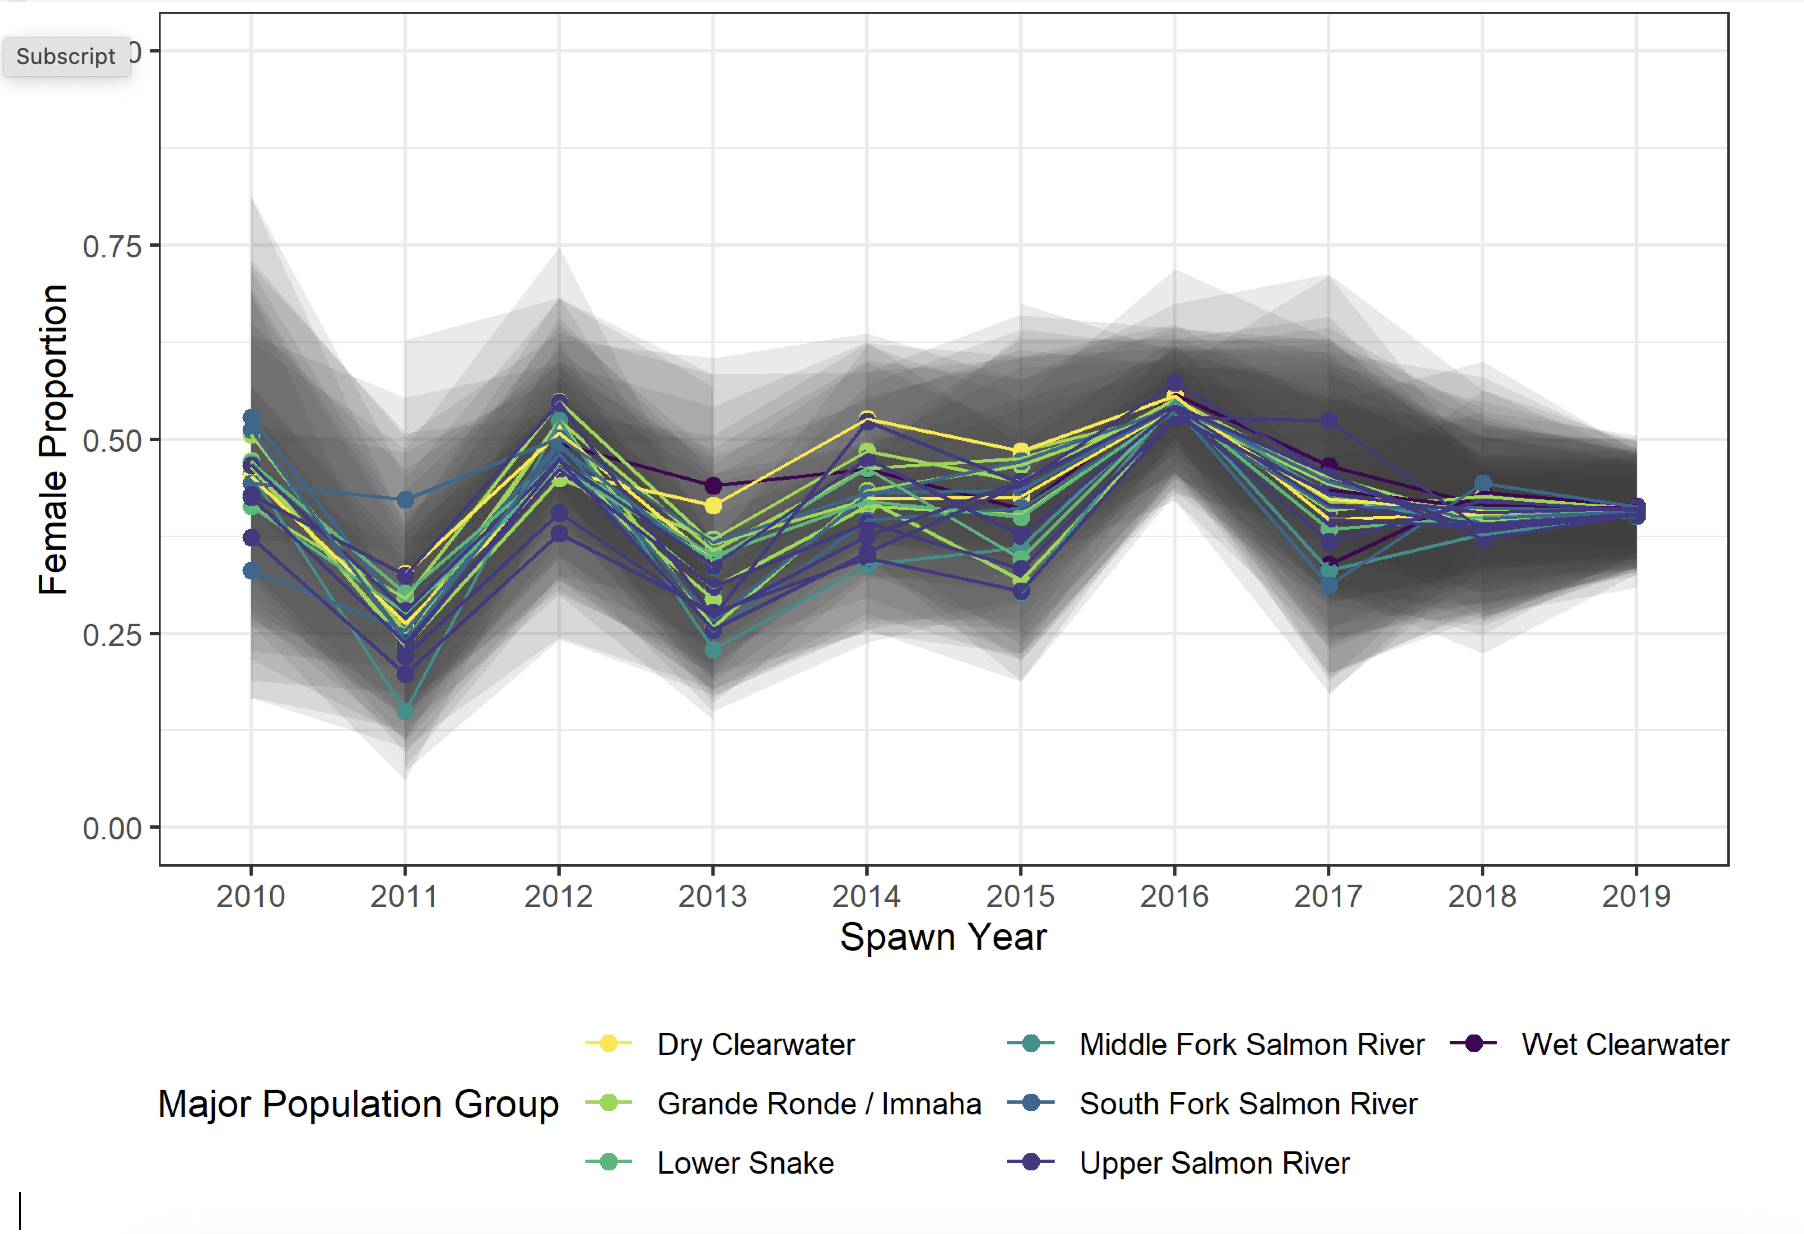
\includegraphics[width=6.01in,height=\textheight]{content/Interior_Columbia/../../media/image23.png}

}

\caption{\label{fig-SnR-DABOM}Natural origin spring/summer Chinook
female proportion (95\% confidence intervals shown in grey) by year and
population (grouped by MPG) as estimated from the state space patch
occupancy model, DABOM. Note that the figure includes non-listed
population groups from the Clearwater River basin, reproduced directly
from IPTDSW 2020.}

\end{figure}

\emph{Population genetic structure}

Sampling of adult Snake River spring/summer Chinook at Lower Granite Dam
and subsequent detections of PIT tags in ICTRT population spawning areas
has allowed the development of a large genetic data set based on SNP
markers (\textbf{iptdsw\_-stream\_2020?}). A neighbor-joining tree
(Figure~\ref{fig-SnR-SS-neighbor-joining-tree}) created from PIT tagged
adults over the spawning years 2010-2019, when combined with reference
GSI baseline samples across the ESU,confirms most of the expected
population structure, with the notable exception of the samples from
fish spawning in the Little Salmon River grouping genetically with the
Upper South Fork Clearwater samples (\textbf{iptdsw\_-stream\_2020?}).

\begin{figure}

{\centering 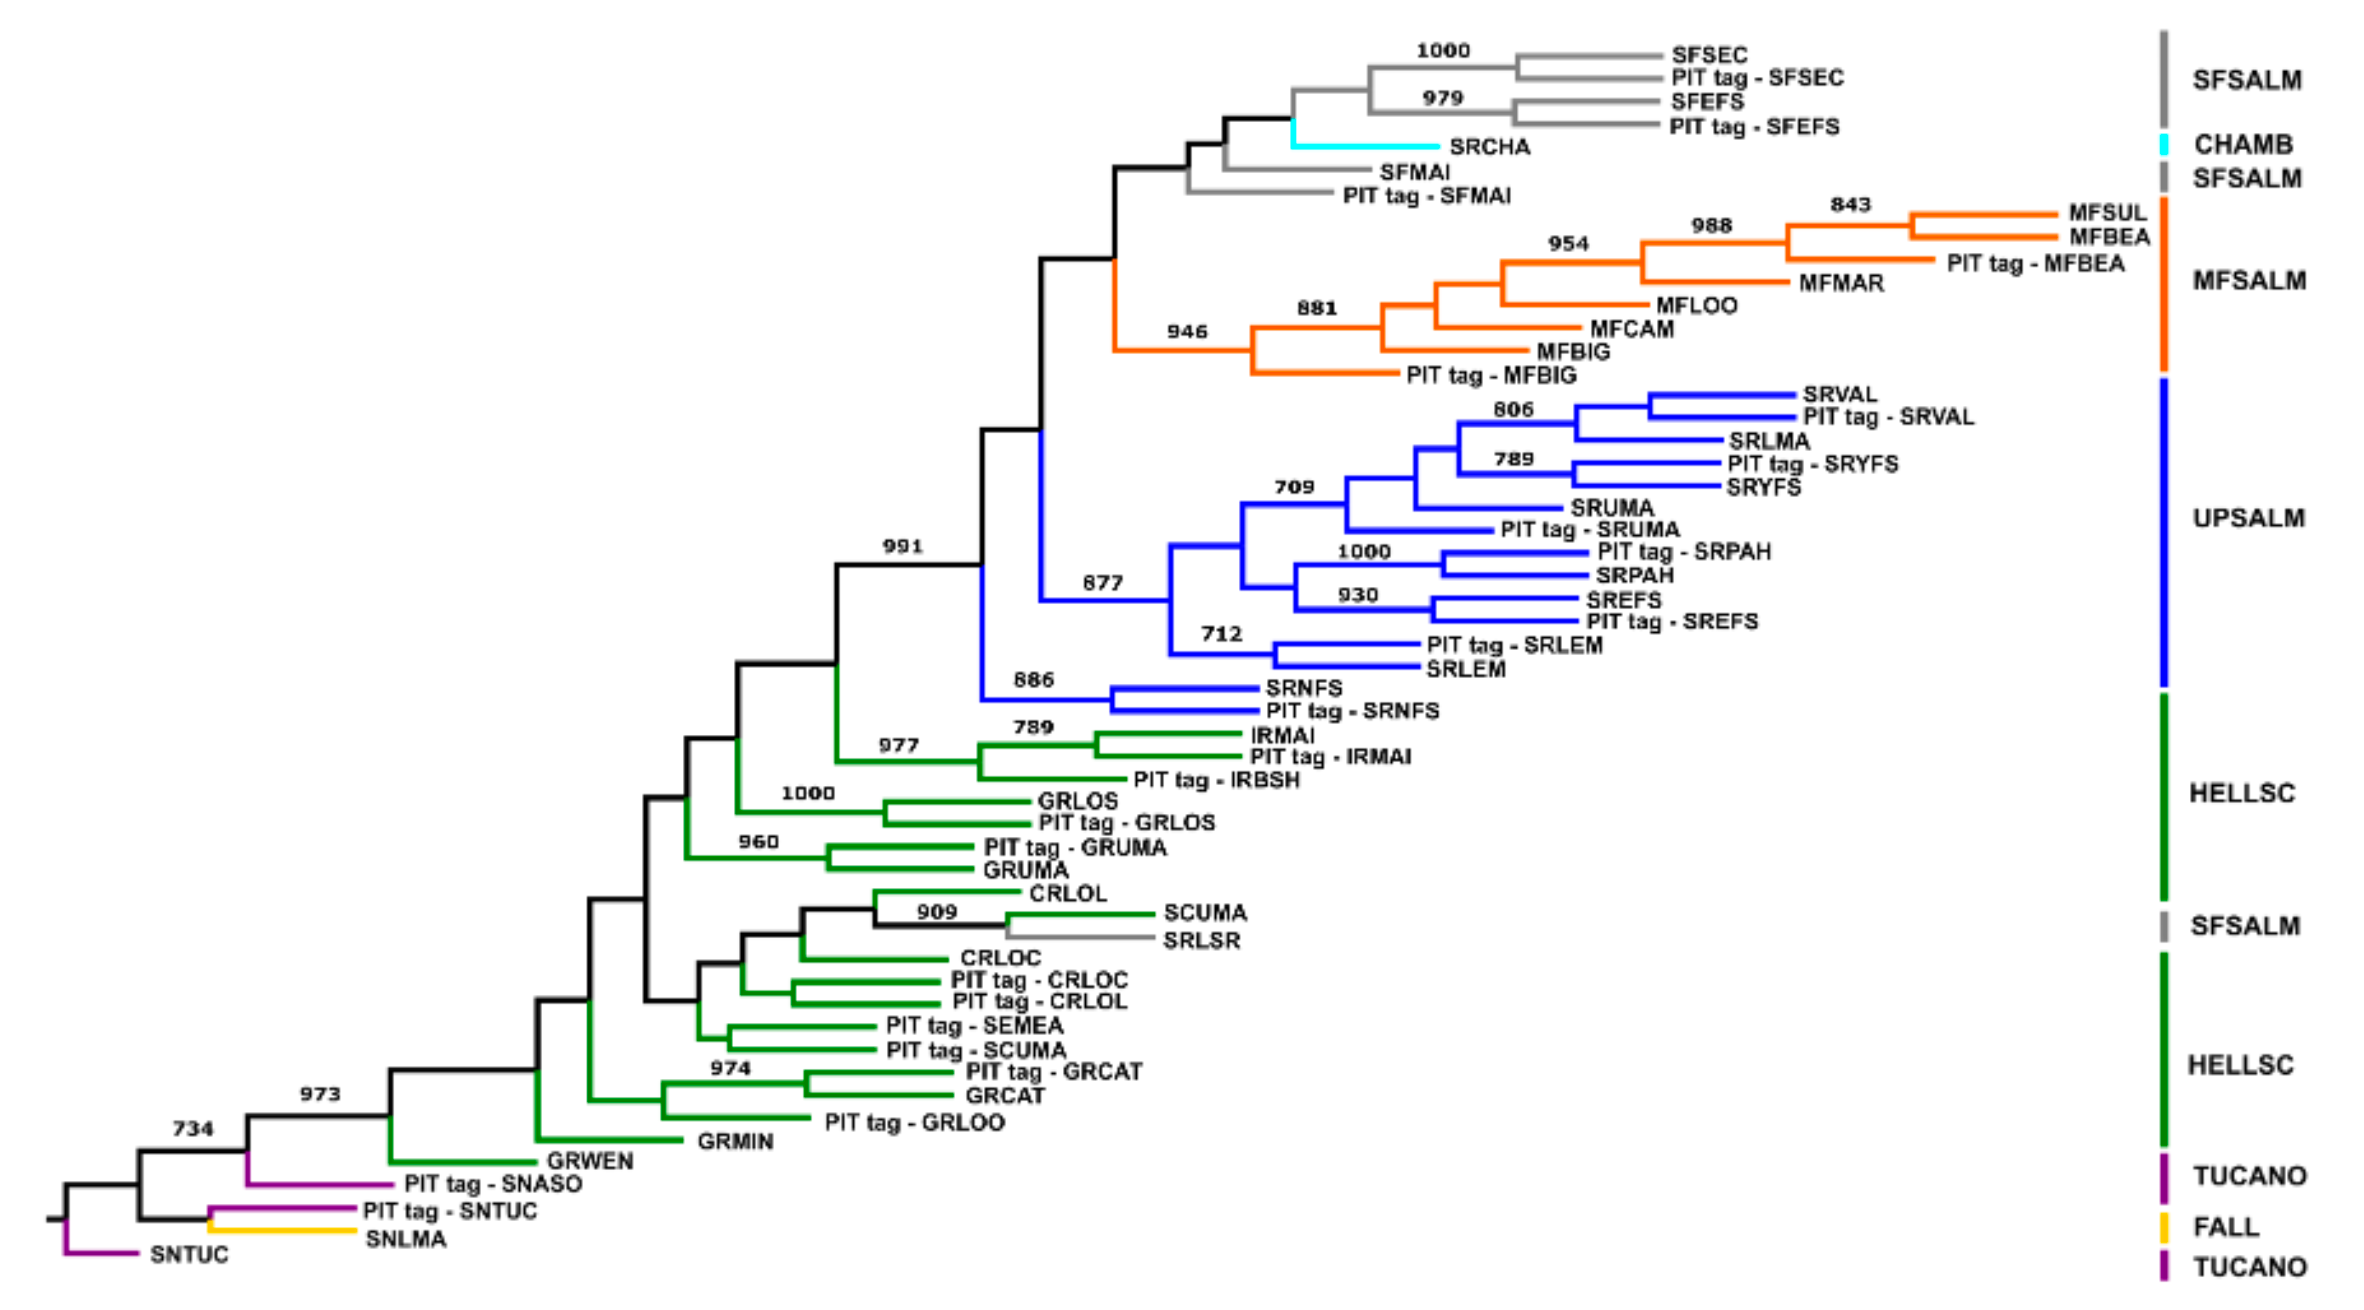
\includegraphics[width=7.88in,height=\textheight]{content/Interior_Columbia/../../media/image24.png}

}

\caption{\label{fig-SnR-SS-neighbor-joining-tree}A neighbor-joining tree
for Snake River Chinook Salmon populations included in the GSI baseline
version 3.1 and collections of PIT tagged returning adults for
SY2010-2019 based on Cavalii-Sforza Edwards chord distance. Bootstrap
support greater than 70\% based on 1,000 replicated are reported. Figure
reproduced from Kinzer et al.~2020.}

\end{figure}

\emph{Spatial structure}

ICTRT criteria for evaluating spatial structure within populations are
based on observing evidence of spawning usage across defined spawning
areas within populations, with an emphasis on historically relatively
large contiguous reaches (major and minor spawning areas). Redd surveys
were conducted by co-managers (NPT, SBT, ODFW, WDFW, IDFG) and the
geolocated redds were aligned with ICTRT identified major and minor
spawning area over the 2015-2019 run years (Felts et al. 2020).
Monitoring occurred in 29 major spawning areas, 13 of which were rated
as occupied, while monitoring of eight minor spawning areas resulted in
only one being rated as occupied. However, non-occupied ratings of mSA
and MSA does not equate to only no spawning as a ``unoccupied'' rating
can also result from patchy spawning not distributed across the entire
reach.

\emph{Ocean Condition Indices}

Snake River spring/summer Chinook salmon are a component of the Columbia
River run that is believed to occupy mid-shelf waters during the early
ocean life history phase. Aggregate annual returns of Columbia River
Spring Chinook are correlated with a range of ocean condition indices
including measures of broad scale physical conditions, local biological
indicators, and local physical factors (Figure 129) (Peterson \emph{et
al.} 2014a). Several indicators, either individually or in combination,
correlate well with spring Chinook salmon adult returns with a lag of 1
to 2 years. However, for each specific indicator or combination, there
are anomalous years that fall outside of the apparent relationships.
Work is continuing to further understand the relationships among
physical and biological `drivers' and annual levels of ocean survival
for salmonid species in the ocean environment. After accounting for age
at return at time of ocean entry, the annual pattern in the Snake River
spring/summer Chinook ESU SAR index generally corresponds to the
composite rankings across ocean indicators available for early ocean
years starting in the late 1990s (Peterson \emph{et al}. 2014).
Indicators of ocean condition are highly correlated with each other, and
exhibit strong temporal autocorrelation (Figure 129, Peterson et al.
(2019)). As a result, when indicators point to conditions that result in
poor ocean productivity for salmonid populations, they do so as a suite
of indicators, and for runs of `good' or `bad' years (see Habitat
chapter). Historically, ocean conditions cycled between periods of high
and low productivity. However, global climate change is likely to
disrupt this pattern, in general, leading to a preponderance of low
productivity years, with an unknown temporal distribution (Crozier et
al. 2020). Recent (2015-2019) ensemble ocean indicators rankings include
four of the worst seven years in the past 20, meaning that an entire
Chinook generation has been subjected to poor ocean productivity
conditions.

\hypertarget{abundance-and-productivity-2}{%
\section{Abundance and
productivity}\label{abundance-and-productivity-2}}

Updated data series on spawner abundance, age structure and
hatchery/natural proportions were used to generate current assessments
of abundance and productivity at the population level. Evaluations were
done using both a set of metrics corresponding to those used in prior
ESA status reviews as well as a set corresponding to the specific
viability criteria based on ICTRT recommendations for this ESU. The
viability review metrics were done consistently across all ESUs and DPSs
to facilitate comparisons across domains. Assessments using the ICTRT
metrics are described in the TRT and Recovery Plan Criteria section
below. The ICTRT abundance and productivity metrics are measured over
longer time frames to dampen the effects of annual variations and they
use annual natural origin age composition to calculate brood year
recruitment when sampling levels meet agency criteria.

Estimates of the annual abundance of natural origin spawners within each
of 27 Snake River Spring Summer Chinook ESU populations are summarized
in five year increments (Table~\ref{tbl-SnR-SS-5-yr-geomeans}) and are
illustrated in Figure~\ref{fig-SnR-SS-smoothed-trends}. The most recent
five year geometric mean abundance estimates for 26 out of the 27
populations are lower than the corresponding estimates for the previous
five year period by varying degrees, the estimate for the
27\textsuperscript{th} population was a slight increase from a very low
abundance in the prior five year period. The entire ESU abundance data
shows a consistent and marked pattern of declining population size, with
the recent five year abundance levels for the 27 populations declining
by an average of 55\%. Medium-term (15 year) population trends in total
spawner abundance were positive over the period 1990 to 2005 for all of
the population natural origin abundance series, and are all declining
over the more recent time interval (2004-2019;
Table~\ref{tbl-SnR-SS-15-yr-trends},
Figure~\ref{fig-SnR-SS-smoothed-trends}). The consistent and sharp
declines for all populations in the ESU are concerning as the abundances
for some populations are approaching similar levels to those of the
early 1990s when the ESU was listed.

\begin{figure}

{\centering 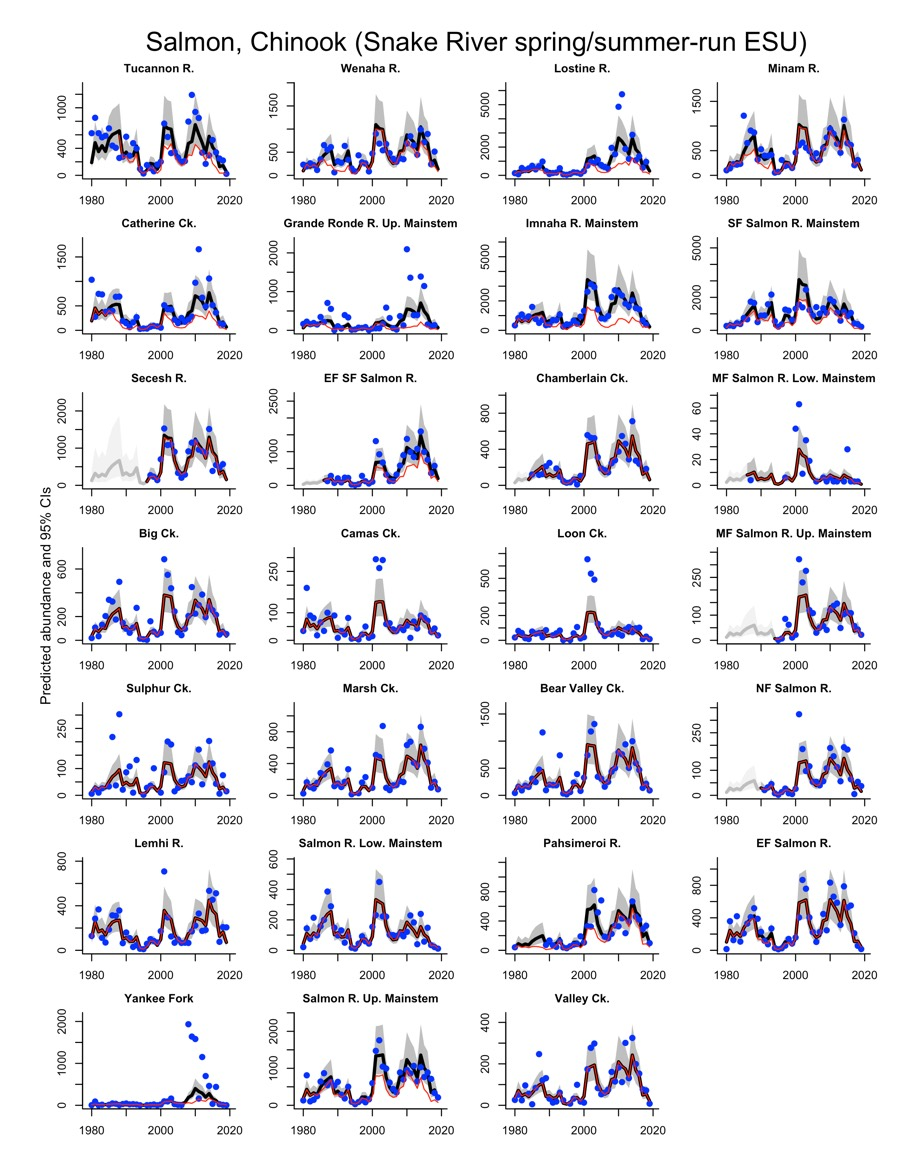
\includegraphics[width=3in,height=\textheight]{content/Interior_Columbia/../../media/image25.jpg}

}

\caption{\label{fig-SnR-SS-smoothed-trends}Smoothed trend in estimated
total (thick black line, with 95\% confidence internal in gray) and
natural (thin red line) population spawning abundance. In portions of a
time series where a population has no annual estimates but smoothed
spawning abundance is estimated from correlations with other populations
the smoothed estimate is shown in light gray. Points show the annual raw
spawning abundance estimates. For some trends the smoothed estimate may
be influenced by earlier data points not included in the plot.}

\end{figure}

\begin{figure}

{\centering 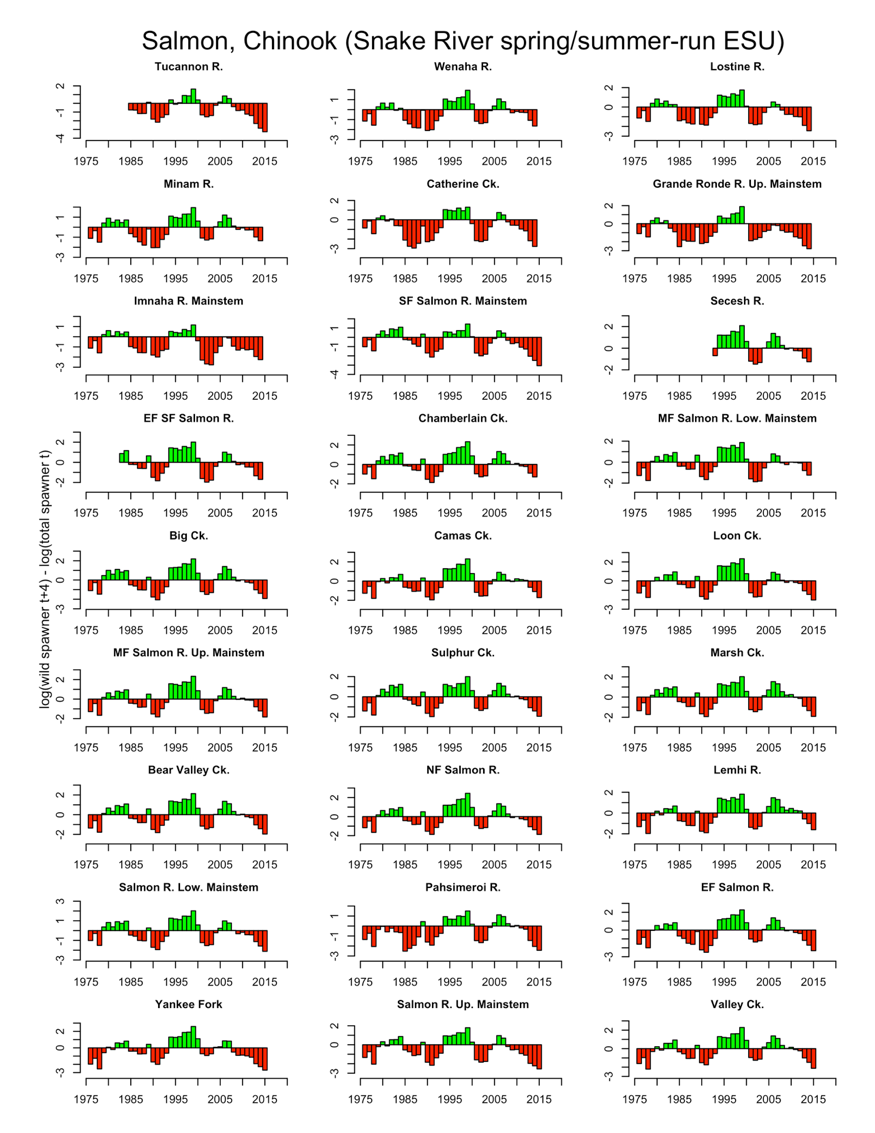
\includegraphics[width=2.92in,height=\textheight]{content/Interior_Columbia/../../media/image26.png}

}

\caption{\label{fig-SnR-SS-productivity-trends}Trends in population
productivity, estimated as the log of the smoothed natural spawning
abundance in year \emph{t} divided by the smoothed natural spawning
abundance in year \emph{t}- 4. Spawning years on x axis.}

\end{figure}

\hypertarget{tbl-SnR-SS-5-yr-geomeans}{}
\begin{longtable}[]{@{}
  >{\raggedright\arraybackslash}p{(\columnwidth - 16\tabcolsep) * \real{0.2081}}
  >{\raggedright\arraybackslash}p{(\columnwidth - 16\tabcolsep) * \real{0.1477}}
  >{\raggedright\arraybackslash}p{(\columnwidth - 16\tabcolsep) * \real{0.0872}}
  >{\raggedright\arraybackslash}p{(\columnwidth - 16\tabcolsep) * \real{0.0805}}
  >{\raggedright\arraybackslash}p{(\columnwidth - 16\tabcolsep) * \real{0.0872}}
  >{\raggedright\arraybackslash}p{(\columnwidth - 16\tabcolsep) * \real{0.0872}}
  >{\raggedright\arraybackslash}p{(\columnwidth - 16\tabcolsep) * \real{0.0940}}
  >{\raggedright\arraybackslash}p{(\columnwidth - 16\tabcolsep) * \real{0.0805}}
  >{\raggedright\arraybackslash}p{(\columnwidth - 16\tabcolsep) * \real{0.0805}}@{}}
\caption{\label{tbl-SnR-SS-5-yr-geomeans}5-year geometric mean of raw
natural spawner counts. This is the raw total spawner count times the
fraction natural estimate, if available. In parentheses, 5-year
geometric mean of raw total spawner counts is shown. A value only in
parentheses means that a total spawner count was available but no or
only one estimate of natural spawners available. The geometric mean was
computed as the product of counts raised to the power 1 over the number
of counts available (2 to 5). A minimum of 2 values were used to compute
the geometric mean. Percent change between the most recent two 5-year
periods is shown on the far right.}\tabularnewline
\toprule()
\begin{minipage}[b]{\linewidth}\raggedright
Population
\end{minipage} & \begin{minipage}[b]{\linewidth}\raggedright
MPG
\end{minipage} & \begin{minipage}[b]{\linewidth}\raggedright
1990-1994
\end{minipage} & \begin{minipage}[b]{\linewidth}\raggedright
1995-1999
\end{minipage} & \begin{minipage}[b]{\linewidth}\raggedright
2000-2004
\end{minipage} & \begin{minipage}[b]{\linewidth}\raggedright
2005-2009
\end{minipage} & \begin{minipage}[b]{\linewidth}\raggedright
2010-2014
\end{minipage} & \begin{minipage}[b]{\linewidth}\raggedright
2015-2019
\end{minipage} & \begin{minipage}[b]{\linewidth}\raggedright
\% Change
\end{minipage} \\
\midrule()
\endfirsthead
\toprule()
\begin{minipage}[b]{\linewidth}\raggedright
Population
\end{minipage} & \begin{minipage}[b]{\linewidth}\raggedright
MPG
\end{minipage} & \begin{minipage}[b]{\linewidth}\raggedright
1990-1994
\end{minipage} & \begin{minipage}[b]{\linewidth}\raggedright
1995-1999
\end{minipage} & \begin{minipage}[b]{\linewidth}\raggedright
2000-2004
\end{minipage} & \begin{minipage}[b]{\linewidth}\raggedright
2005-2009
\end{minipage} & \begin{minipage}[b]{\linewidth}\raggedright
2010-2014
\end{minipage} & \begin{minipage}[b]{\linewidth}\raggedright
2015-2019
\end{minipage} & \begin{minipage}[b]{\linewidth}\raggedright
\% Change
\end{minipage} \\
\midrule()
\endhead
Tucannon R. & Low. Snake & 230 (314) & 34 (84) & 226 (398) & 276 (403) &
285 (422) & 47 (185) & -84 (-56) \\
Wenaha R. & Grande Ronde/Imnaha & 71 (305) & 164 (186) & 612 (638) & 354
(364) & 507 (698) & 383 (529) & -24 (-24) \\
Lostine R. & Grande Ronde/Imnaha & 82 (159) & 105 (108) & 398 (711) &
340 (899) & 1024 (2807) & 366 (925) & -64 (-67) \\
Minam R. & Grande Ronde/Imnaha & 110 (284) & 162 (166) & 541 (552) & 449
(460) & 684 (765) & 375 (401) & -45 (-48) \\
Catherine Ck. & Grande Ronde/Imnaha & 0 (102) & 59 (59) & 124 (256) & 71
(209) & 430 (890) & 85 (237) & -80 (-73) \\
Grande Ronde R. Up. Mainstem & Grande Ronde/Imnaha & 33 (96) & 32 (32) &
54 (103) & 22 (109) & 155 (906) & 51 (218) & -67 (-76) \\
Imnaha R. Mainstem & Grande Ronde/Imnaha & 214 (551) & 270 (536) & 938
(2142) & 286 (1308) & 685 (2055) & 352 (866) & -49 (-58) \\
SF Salmon R. Mainstem & SF Salmon & 690 (1089) & 344 (602) & 968 (1540)
& 628 (1128) & 913 (1184) & 160 (497) & -82 (-58) \\
Secesh R. & SF Salmon & (NA) & 187 (206) & 997 (1028) & 435 (459) & 1043
(1064) & 468 (489) & -55 (-54) \\
EF SF Salmon R. & SF Salmon & 116 (116) & 49 (50) & 369 (487) & 129
(308) & 709 (1147) & 359 (629) & -49 (-45) \\
Chamberlain Ck. & MF Salmon & 121 (121) & 35 (35) & 468 (468) & 198
(198) & 454 (454) & 228 (228) & -50 (-50) \\
MF Salmon R. Low. Mainstem & MF Salmon & (NA) & (NA) & 28 (28) & 4 (4) &
4 (4) & 5 (5) & 25 (25) \\
Big Ck. & MF Salmon & 76 (76) & 29 (29) & 302 (302) & 121 (121) & 270
(270) & 99 (99) & -63 (-63) \\
Camas Ck. & MF Salmon & 20 (20) & 13 (13) & 115 (115) & 43 (43) & 42
(42) & 42 (42) & 0 (0) \\
Loon Ck. & MF Salmon & 25 (25) & 21 (21) & 225 (225) & 54 (54) & 65 (65)
& 31 (31) & -52 (-52) \\
MF Salmon R. Up. Mainstem & MF Salmon & (NA) & 13 (13) & 140 (140) & 52
(52) & 104 (104) & 58 (58) & -44 (-44) \\
Sulphur Ck. & MF Salmon & 59 (59) & 21 (21) & 55 (55) & 49 (49) & 112
(112) & 32 (32) & -71 (-71) \\
Marsh Ck. & MF Salmon & 102 (102) & 99 (99) & 285 (285) & 126 (126) &
563 (563) & 197 (197) & -65 (-65) \\
Bear Valley Ck. & MF Salmon & 177 (177) & 95 (95) & 662 (662) & 305
(305) & 777 (777) & 236 (236) & -70 (-70) \\
NF Salmon R. & Up. Salmon & 22 (22) & 8 (8) & 112 (112) & 59 (59) & 129
(129) & 41 (41) & -68 (-68) \\
Lemhi R. & Up. Salmon & 51 (51) & 51 (51) & 198 (198) & 86 (86) & 262
(262) & 238 (238) & -9 (-9) \\
Salmon R. Low. Mainstem & Up. Salmon & 63 (63) & 41 (41) & 239 (239) &
99 (99) & 137 (137) & 37 (37) & -73 (-73) \\
Pahsimeroi R. & Up. Salmon & 22 (73) & 45 (73) & 173 (343) & 209 (275) &
360 (387) & 132 (283) & -63 (-27) \\
EF Salmon R. & Up. Salmon & 69 (108) & 34 (46) & 442 (442) & 224 (224) &
602 (602) & 138 (138) & -77 (-77) \\
Yankee Fork & Up. Salmon & 16 (16) & 6 (6) & 60 (60) & 25 (120) & 169
(623) & 22 (24) & -87 (-96) \\
Salmon R. Up. Mainstem & Up. Salmon & 227 (275) & 68 (86) & 671 (1100) &
326 (566) & 628 (898) & 170 (509) & -73 (-43) \\
Valley Ck. & Up. Salmon & 26 (26) & 26 (26) & 109 (109) & 85 (85) & 192
(192) & 67 (67) & -65 (-65) \\
\bottomrule()
\end{longtable}

\hypertarget{tbl-SnR-SS-15-yr-trends}{}
\begin{longtable}[]{@{}
  >{\raggedright\arraybackslash}p{(\columnwidth - 6\tabcolsep) * \real{0.3131}}
  >{\raggedright\arraybackslash}p{(\columnwidth - 6\tabcolsep) * \real{0.2222}}
  >{\raggedright\arraybackslash}p{(\columnwidth - 6\tabcolsep) * \real{0.2121}}
  >{\raggedright\arraybackslash}p{(\columnwidth - 6\tabcolsep) * \real{0.2323}}@{}}
\caption{\label{tbl-SnR-SS-15-yr-trends}15-year trends in log natural
spawner abundance computed from a linear regression applied to the
smoothed wild spawner log abundance estimate. Only populations with at
least 4 wild spawner estimates from 1980 to 2014 are shown and with at
least 2 data points in the first 5 years and last 5 years of the 15-year
period.}\tabularnewline
\toprule()
\begin{minipage}[b]{\linewidth}\raggedright
Population
\end{minipage} & \begin{minipage}[b]{\linewidth}\raggedright
MPG
\end{minipage} & \begin{minipage}[b]{\linewidth}\raggedright
1990-2005
\end{minipage} & \begin{minipage}[b]{\linewidth}\raggedright
2004-2019
\end{minipage} \\
\midrule()
\endfirsthead
\toprule()
\begin{minipage}[b]{\linewidth}\raggedright
Population
\end{minipage} & \begin{minipage}[b]{\linewidth}\raggedright
MPG
\end{minipage} & \begin{minipage}[b]{\linewidth}\raggedright
1990-2005
\end{minipage} & \begin{minipage}[b]{\linewidth}\raggedright
2004-2019
\end{minipage} \\
\midrule()
\endhead
Tucannon R. & Low. Snake & 0.04 (-0.07, 0.15) & -0.13 (-0.23, -0.04) \\
Wenaha R. & Grande Ronde/Imnaha & 0.17 (0.08, 0.26) & -0.04 (-0.11,
0.02) \\
Lostine R. & Grande Ronde/Imnaha & 0.12 (0.03, 0.21) & 0 (-0.09,
0.09) \\
Minam R. & Grande Ronde/Imnaha & 0.12 (0.03, 0.21) & -0.03 (-0.1,
0.03) \\
Catherine Ck. & Grande Ronde/Imnaha & 0.11 (0.03, 0.2) & -0.01 (-0.12,
0.1) \\
Grande Ronde R. Up. Mainstem & Grande Ronde/Imnaha & 0.08 (-0.01, 0.17)
& 0.01 (-0.06, 0.09) \\
Imnaha R. Mainstem & Grande Ronde/Imnaha & 0.1 (0.01, 0.19) & -0.02
(-0.09, 0.05) \\
SF Salmon R. Mainstem & SF Salmon & 0.07 (-0.03, 0.16) & -0.12 (-0.21,
-0.03) \\
Secesh R. & SF Salmon & & -0.02 (-0.09, 0.05) \\
EF SF Salmon R. & SF Salmon & 0.11 (0, 0.21) & 0.05 (-0.03, 0.13) \\
Chamberlain Ck. & MF Salmon & 0.11 (0, 0.21) & -0.02 (-0.09, 0.05) \\
MF Salmon R. Low. Mainstem & MF Salmon & & -0.08 (-0.14, -0.02) \\
Big Ck. & MF Salmon & 0.1 (-0.01, 0.21) & -0.03 (-0.11, 0.04) \\
Camas Ck. & MF Salmon & 0.11 (0, 0.22) & -0.03 (-0.09, 0.03) \\
Loon Ck. & MF Salmon & 0.14 (0.03, 0.25) & -0.08 (-0.14, -0.01) \\
MF Salmon R. Up. Mainstem & MF Salmon & & -0.03 (-0.1, 0.04) \\
Sulphur Ck. & MF Salmon & 0.07 (-0.03, 0.17) & -0.03 (-0.11, 0.04) \\
Marsh Ck. & MF Salmon & 0.08 (-0.02, 0.19) & 0.01 (-0.07, 0.09) \\
Bear Valley Ck. & MF Salmon & 0.11 (0.01, 0.21) & -0.03 (-0.11, 0.04) \\
NF Salmon R. & Up. Salmon & 0.13 (0.02, 0.24) & -0.03 (-0.11, 0.04) \\
Lemhi R. & Up. Salmon & 0.09 (-0.02, 0.19) & 0.04 (-0.03, 0.11) \\
Salmon R. Low. Mainstem & Up. Salmon & 0.08 (-0.02, 0.19) & -0.09
(-0.16, -0.02) \\
Pahsimeroi R. & Up. Salmon & 0.16 (0.07, 0.25) & -0.02 (-0.12, 0.07) \\
EF Salmon R. & Up. Salmon & 0.14 (0.03, 0.26) & -0.05 (-0.14, 0.03) \\
Yankee Fork & Up. Salmon & 0.14 (0.02, 0.25) & -0.02 (-0.11, 0.06) \\
Salmon R. Up. Mainstem & Up. Salmon & 0.08 (-0.02, 0.18) & -0.06 (-0.14,
0.02) \\
Valley Ck. & Up. Salmon & 0.12 (0.01, 0.22) & -0.03 (-0.1, 0.05) \\
\bottomrule()
\end{longtable}

Smolt to adult return survival estimates (SARs) are generated by the
Columbia River Data Access in Real Time (CBR and UW 2020) project using
PIT tag detections from all release locations within each population
basin (Columbia River DART, 2020). The SAR indices represent cumulative
marine, nearshore and estuary survival. shows the geometric mean of R/S
and SAR indices for the stocks available across five MPGs in the ESU. In
general, these broad-brush descriptors of population processes indicate
relatively poor ocean survival for the Salmon River MPGs and relatively
poor freshwater productivity for the Grande Ronde and Lower Snake River
MPGs. Using the R/S and SAR indicators by population, it is possible to
generate an indicator of fresh water productivity (FWPI) as a ratio of
R/S and SAR. This quantity can be thought of as an indicator of smolts
per spawner, and thus, the overall population productivity in the
freshwater environment. An FWPI score of \textgreater100 should indicate
healthy fresh water productivity (roughly 100 smolts per female). The
initial assessment by the (\textbf{noauthor\_ictrt\_2007?}) ICTRT (2007)
identified significant abundance/productivity gaps for this ESU. In
general, populations within Grande Ronde and Lower Snake River MPG are
still showing the lowest productivity.

\begin{figure}

{\centering 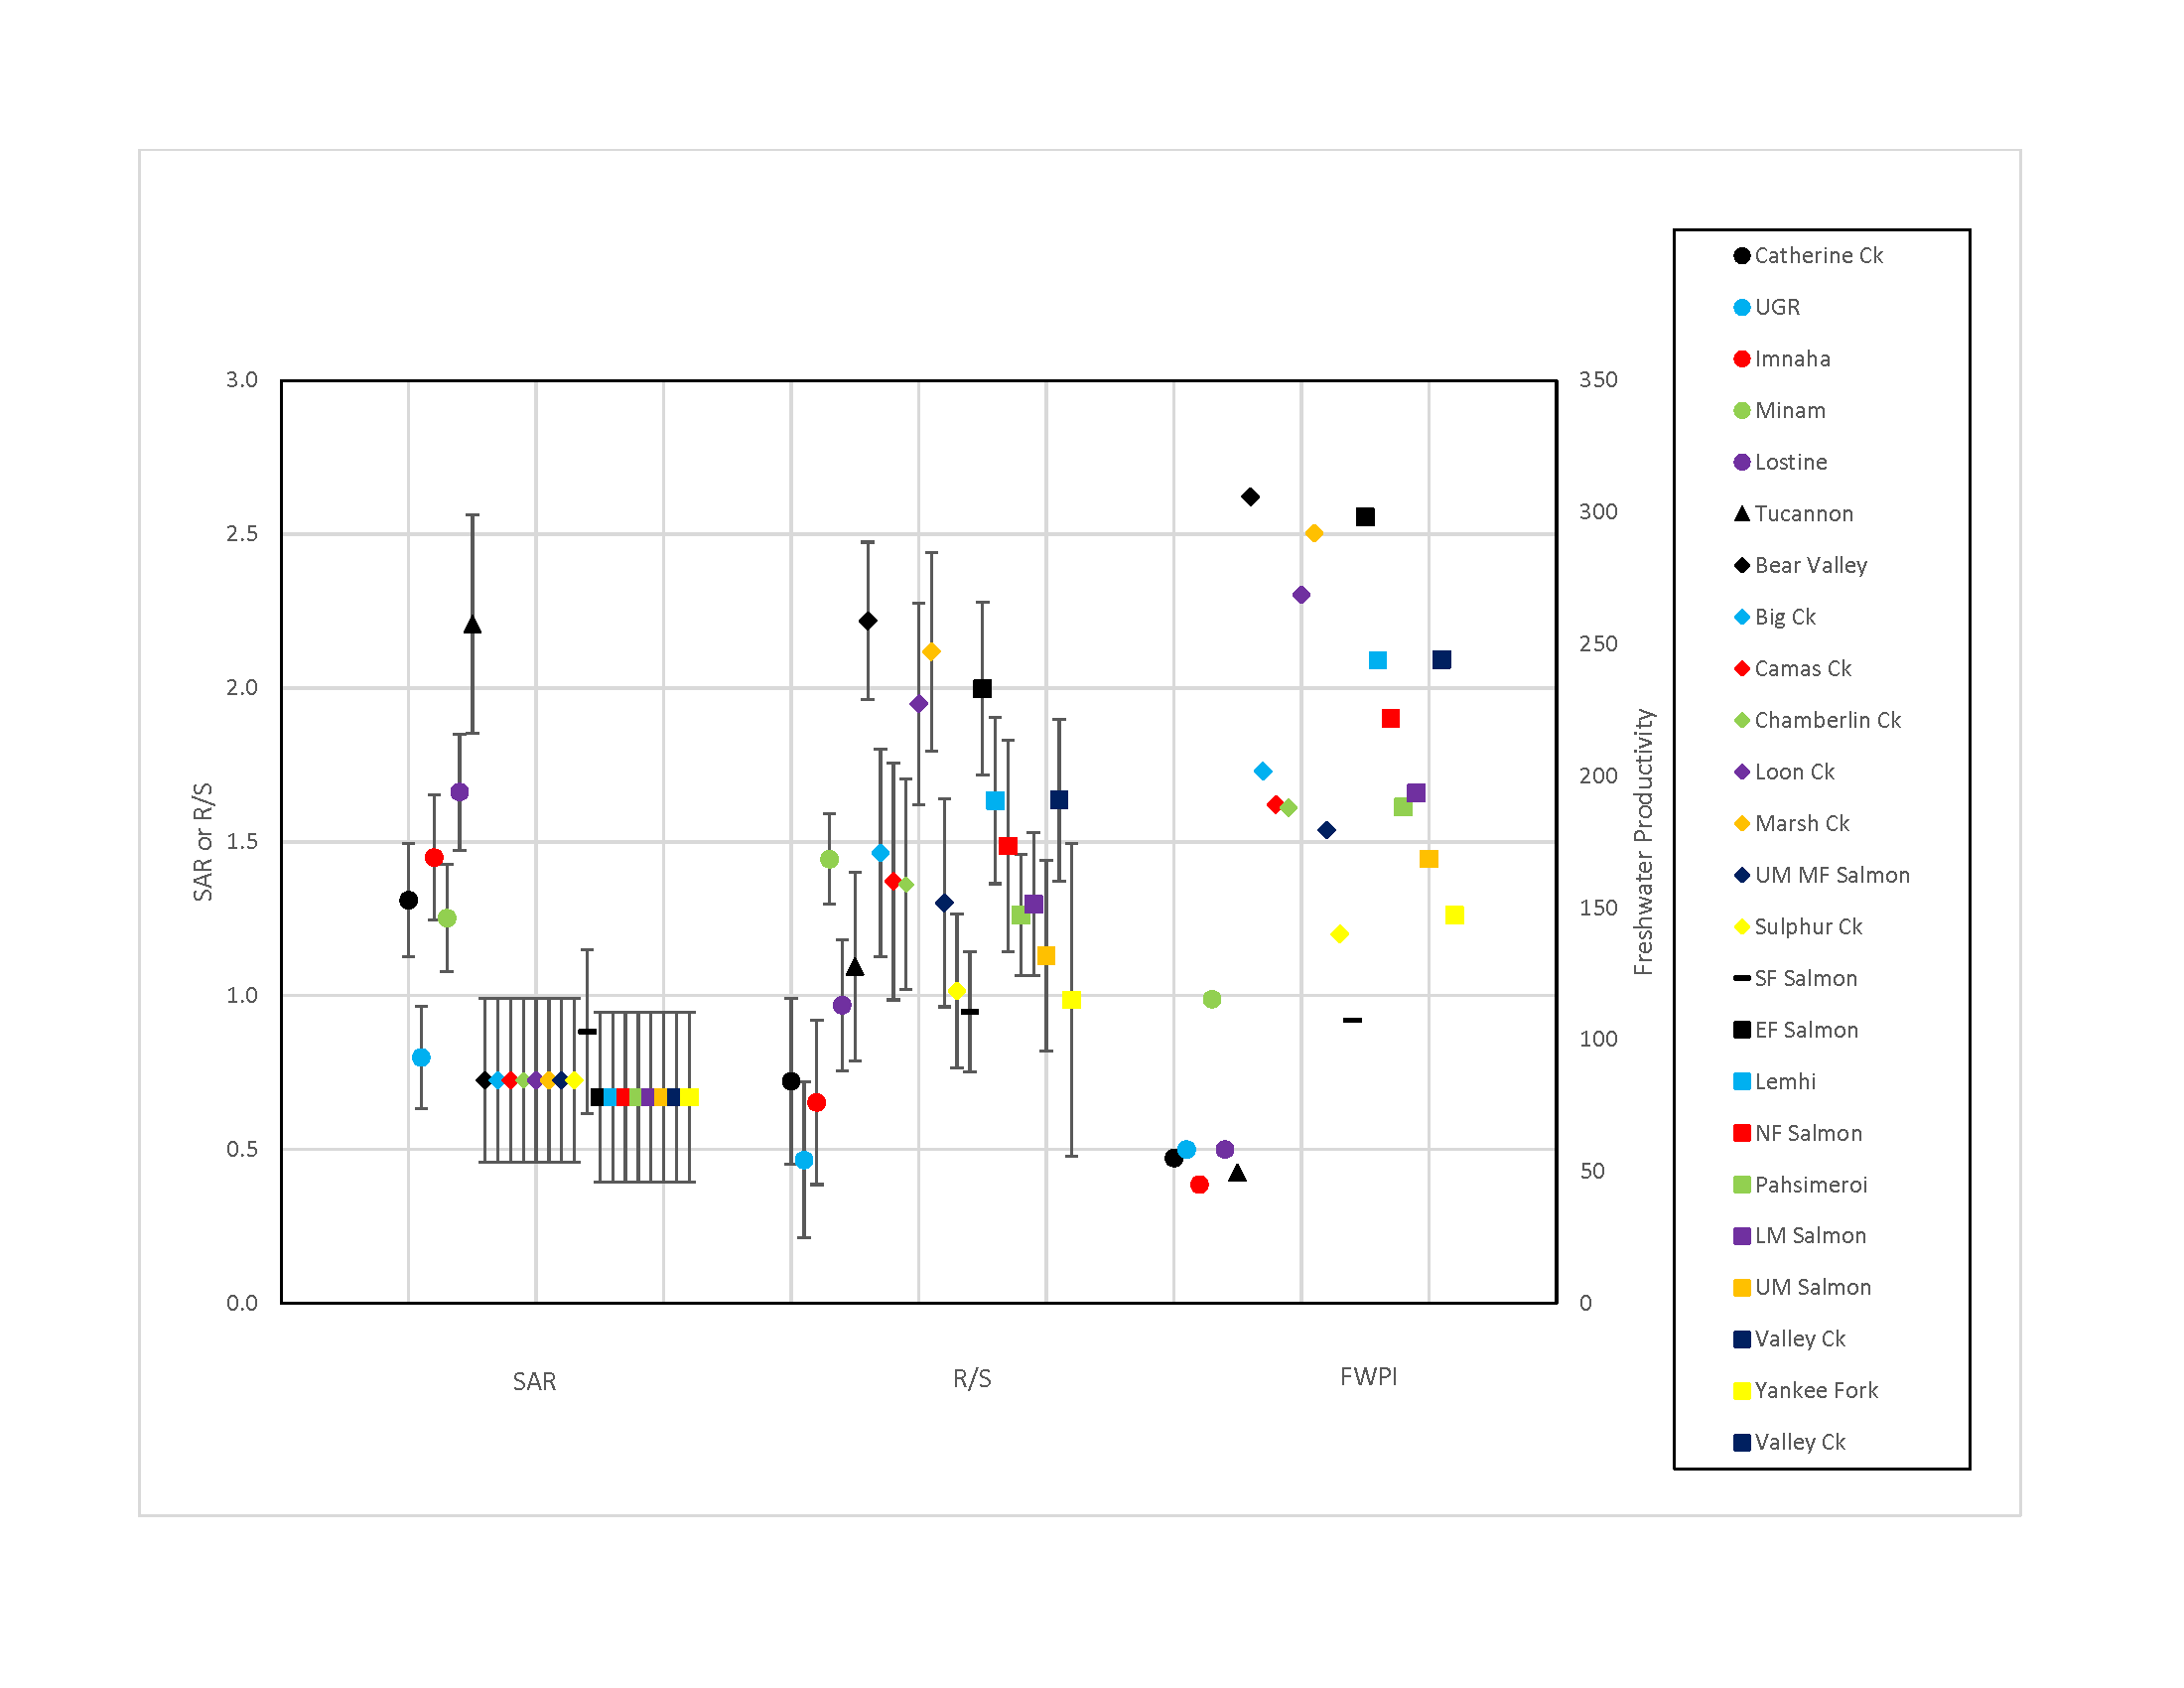
\includegraphics[width=7.33in,height=\textheight]{content/Interior_Columbia/../../media/image27.png}

}

\caption{\label{fig-SnR-SS-smolt-to-adults}Smolt to Adult Return,
Recruits per Spawner, and Freshwater Productivity Index (FWPI) for each
of the populations in the ESU. Geometric means of SAR and R/S are shown
for each population, along with the standard error of the estimate
(whiskers represent +/- one standard error). The time period included in
the SAR or R/S indices is the past 20 years, depending on data
availability. The FWPI is constructed as a ratio of the geomean R/S and
SAR, and can be thought of as a measure of smolts per spawner.}

\end{figure}

\hypertarget{non-treaty-harvest-2}{%
\section{Non-treaty Harvest}\label{non-treaty-harvest-2}}

Harvest impacts on the spring component of this ESU are essentially the
same as those on the Upper Columbia River
(Figure~\ref{fig-SnR-SS-non-treaty-exploitation}). Harvest occurs in the
lower portion of the mainstem Columbia River. Mainstem Columbia River
fisheries represent the majority of harvest impacts on this ESU. In some
years additional harvest in the Snake River basin on specific
populations within the ESU occurs. Snake River summer Chinook share the
ocean distribution patterns of the upper basin spring runs and are only
subject to significant harvest in the mainstem Columbia River. Harvest
of summer Chinook has been more constrained than that of spring Chinook
with consequently lower exploitation rates on the summer component of
this ESU. However, the overall pattern of exploitation rates calculated
by the TAC is nearly identical to that of the Upper Columbia River
spring Chinook.

\begin{figure}

{\centering 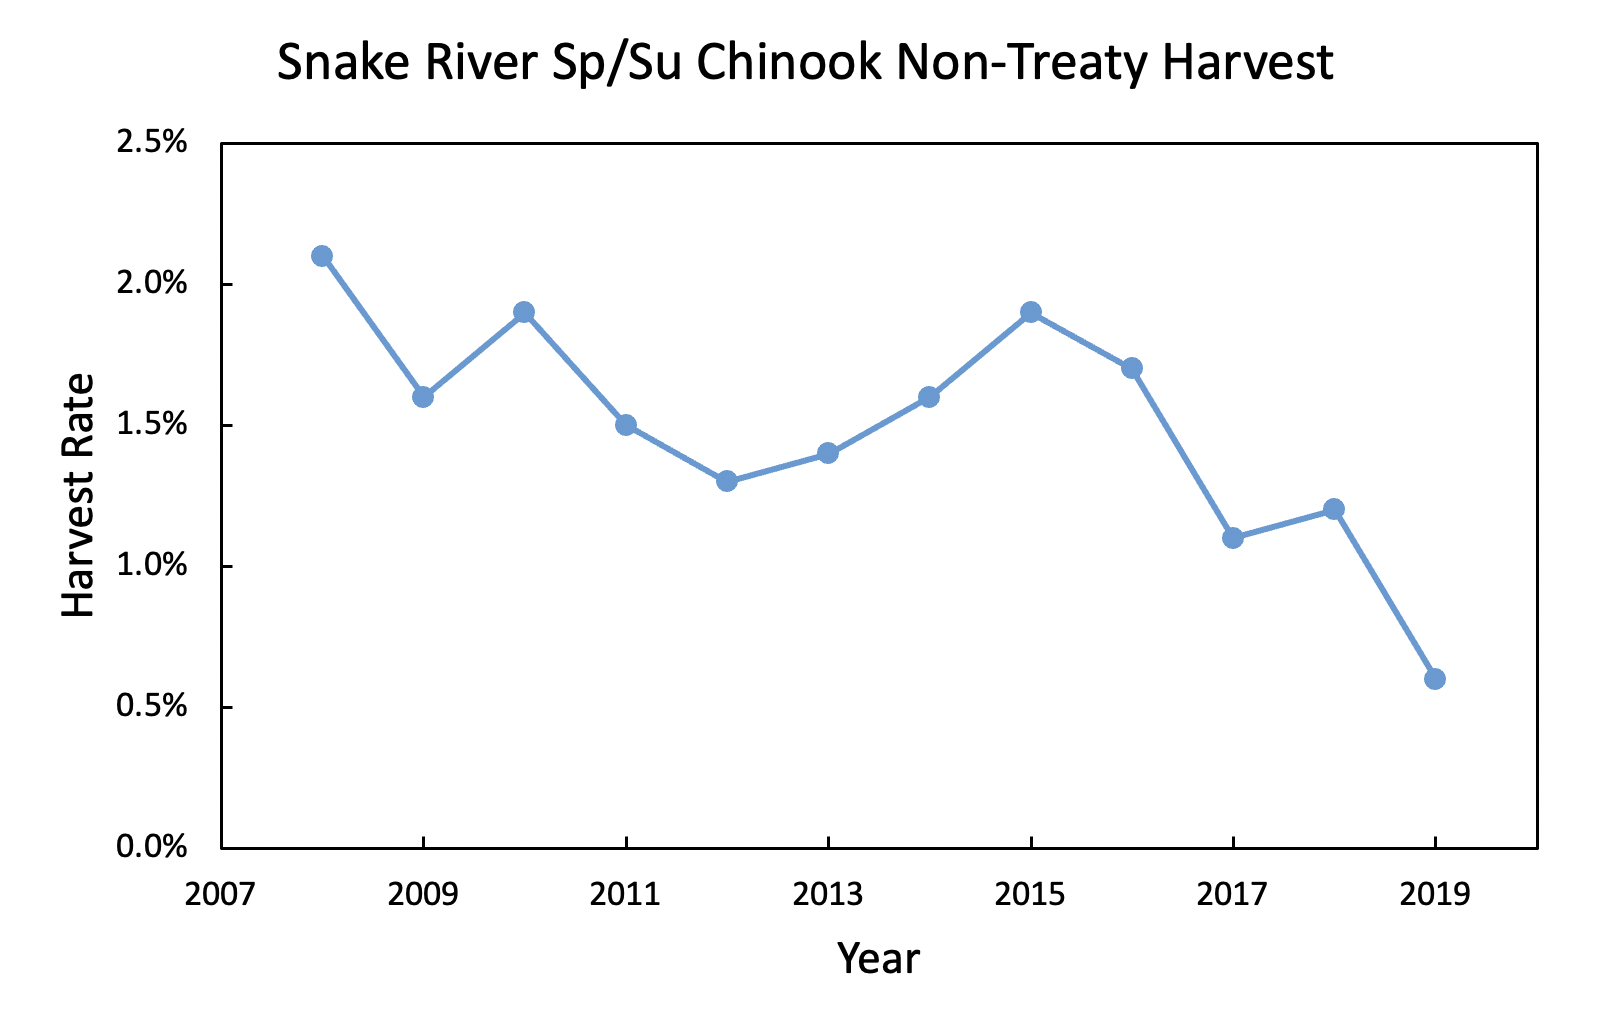
\includegraphics[width=5.39in,height=\textheight]{content/Interior_Columbia/../../media/image27b.png}

}

\caption{\label{fig-SnR-SS-non-treaty-exploitation}Non-treaty
exploitation rates for Snake River spring/summer Chinook salmon in the
mainstem Columbia River fisheries. Data from the Columbia River
Technical Advisory Team (TAC 2015).(TAC 2020)}

\end{figure}

\hypertarget{spatial-structure-and-diversity-2}{%
\section{Spatial structure and
diversity}\label{spatial-structure-and-diversity-2}}

Current estimates of spatial structure and diversity ratings for Snake
River Spring/Summer Chinook populations are summarized in Table 14. The
ICTRT ratings for spatial structure remain unchanged. Most population
abundance estimates are based on redd or weir counts conducted across
reaches within or across major spawning areas. Recent survey results are
consistent with records for the years analyzed by the ICTRT.

The proportion of hatchery origin spawners within populations varies
considerably across MPGs (Figure~\ref{fig-SnR-SS-smoothed-frac-wild},
Table~\ref{tbl-SnR-SS-5-yr-fracwild}). All five extant populations in
the Grande Ronde River basin had relatively high hatchery spawner
proportions in the 1990s, reflecting the large scale use of out of basin
stock (Rapid River) in local releases during that period. Managers
transitioned the release programs to incorporate local natural origin
brood stock in the mid 1990s. Currently five of the six extant natural
population tributaries as well as Lookingglass Creek (with an extripated
natal population) have targeted hatchery releases. During that
transition, returning hatchery origin fish from the Rapid River releases
were actively removed prior to spawning. Returns from natural origin
broodstock increased as the specific in-basin programs reached their
smolt production objectives. The current local broodstock based hatchery
programs in three of the basins are designed to supplement natural
spawning while contributing to meeting mitigation objectives. Releases
into Lookingglass Creek, an extirpated population, are a conventional
segregated program. The historical Lookingglass Creek run is believed to
have been extirpated as a result of the out of basin hatchery program.
The current program uses broodstock that originated from Catherine
Creek. The Minam and Wenaha River populations do not have direct
supplementation programs. The Imnaha River, an adjacent river basin to
the Grande Ronde, is also in this MPG, has an ongoing integrated
hatchery program that incorporates natural origin broodstock.

The single current extant population in the Lower Snake River MPG, the
Tucannon River, has an ongoing supplementation program, and hatchery
returns have constituted about a third of spawning in natural areas in
recent years. Mark recapture estimates compared to redd count and
carcass recoveries indicate that prespawn mortalities in the Tucannon
River have been relatively high in recent years. Efforts are underway to
further quantify and to identify potential direct causes (Bumgarner and
Dedloff 2015). Hatchery proportions for populations in the Middle Fork
Salmon MPG are based on carcass recoveries and remain very low,
indicating negligible straying rates as there are no direct release
programs in this river basin.

Three of the four South Fork Salmon MPG populations have ongoing
hatchery programs. Hatchery proportions for the two of the three
populations in the South Fork Salmon River with active hatchery programs
decreased marginally in the most recent five year update. The Secesh
River continues to show low hatchery proportions reflecting some
straying from the programs in the adjacent populations. Integrated
hatchery programs are now being implemented in parallel to ongoing
production (segregated) operations in the South Fork and East Fork of
the South Fork Salmon River facilities. The ICTRT included a fourth
population in the neighboring Little Salmon River drainage in this MPG.
This population includes returns from large scale hatchery releases
although some of its side tributary spawning areas likely have low
hatchery contributions. Direct estimates of natural origin spawners for
this population are limited to weir passage counts for the Rapid River
tributary.

In the Upper Salmon River MPG, four of the seven populations with
sufficient information to directly estimate hatchery contributions had
very low hatchery proportions (Lemhi River, East Fork Salmon River,
Valley Creek and the Lower Mainstem Salmon River). The most recent five
year mean for the Pahsimeroi River was also relatively low. Both of the
hatchery facilities in this MPG are operating parallel integrated and
segregated programs. Two of the other populations in this MPG are the
subject of active hatchery release programs as reflected in their
respective average spawner proportions. Hatchery contributions to
spawning in the bulk of the habitat used by the Upper Salmon River
population are regulated by managing passage at Sawtooth weir, located
on the mainstem Salmon River near the downstream extent of spawning.
Releases of any origin fish (integrated/segregated) has occurred above
the weirs at both the USR and PAH facilities to meet escapement goals
due to recent low returns. Clearly, pHOS in these populations will be
impacted, but operating agreement balances the risks associated with
introgression with depensation at very low run sizes. Hatchery
proportions within the Yankee Fork population have increased
substantially in recent years, reflecting returns from a large scale
supplementation effort conducted by the Shosonne Bannock tribal
fisheries department. In some recent years the program has augmented
ongoing smolt releases with adult plants in the Yankee Fork and egg
boxes in Panther Creek, when there are surplus returns from the Sawtooth
Hatchery program in the Upper Salmon River Denny and Blackadar (2015).
Recent efforts to evaluate the origin of the Panther Creek spawning
population has shown a mixture of potentially long term occupants (close
to MFSR) and clear hatchery origin stocks (SFSR, Rapid River, USR, and
PAH).

\begin{figure}

{\centering 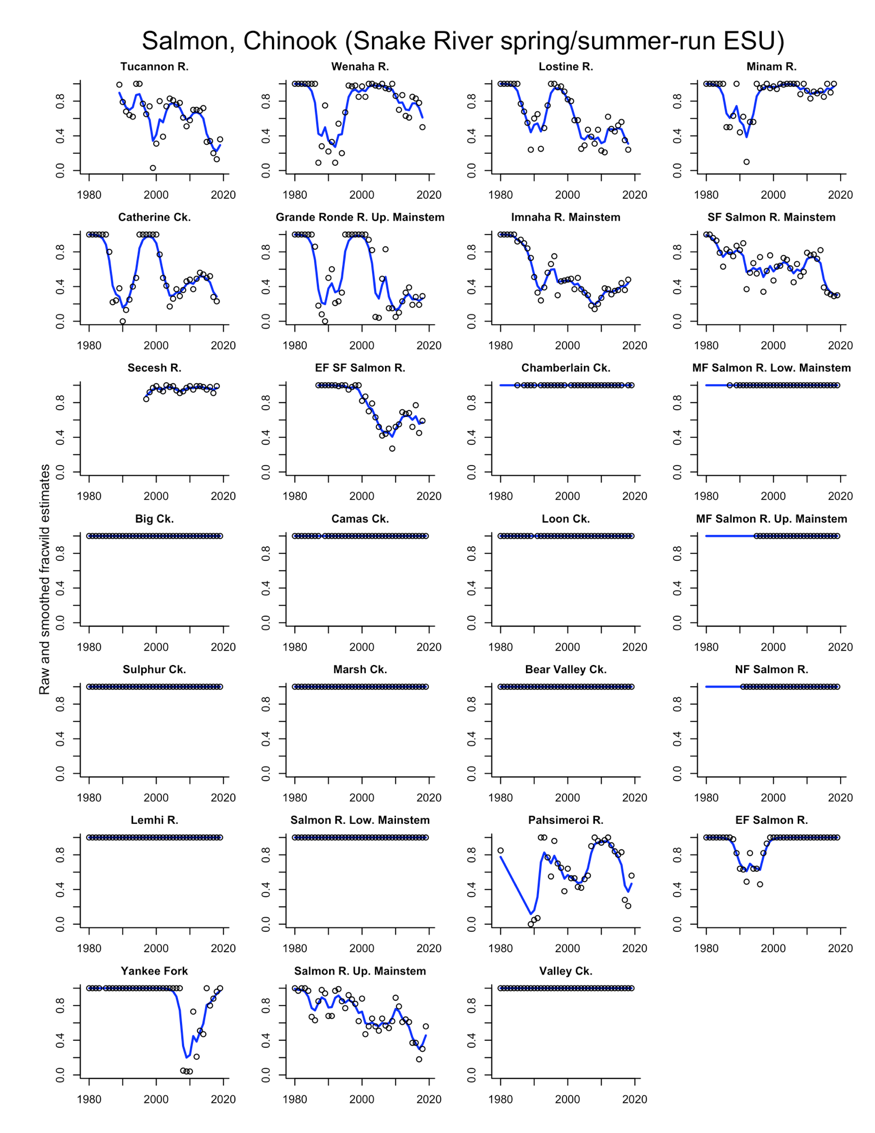
\includegraphics[width=2.92in,height=\textheight]{content/Interior_Columbia/../../media/image28.png}

}

\caption{\label{fig-SnR-SS-smoothed-frac-wild}Smoothed trend in the
estimated fraction of the natural spawning population consisting of fish
if natural origin. Points show the annual raw estimates.}

\end{figure}

\hypertarget{tbl-SnR-SS-5-yr-fracwild}{}
\begin{longtable}[]{@{}
  >{\raggedright\arraybackslash}p{(\columnwidth - 10\tabcolsep) * \real{0.3263}}
  >{\raggedright\arraybackslash}p{(\columnwidth - 10\tabcolsep) * \real{0.1263}}
  >{\raggedright\arraybackslash}p{(\columnwidth - 10\tabcolsep) * \real{0.1263}}
  >{\raggedright\arraybackslash}p{(\columnwidth - 10\tabcolsep) * \real{0.1263}}
  >{\raggedright\arraybackslash}p{(\columnwidth - 10\tabcolsep) * \real{0.1263}}
  >{\raggedright\arraybackslash}p{(\columnwidth - 10\tabcolsep) * \real{0.1263}}@{}}
\caption{\label{tbl-SnR-SS-5-yr-fracwild}5-year mean of fraction natural
origin spawners (sum of all estimates divided by the number of
estimates). Blanks mean no estimate available in that 5-year
range.}\tabularnewline
\toprule()
\begin{minipage}[b]{\linewidth}\raggedright
Population
\end{minipage} & \begin{minipage}[b]{\linewidth}\raggedright
1995-1999
\end{minipage} & \begin{minipage}[b]{\linewidth}\raggedright
2000-2004
\end{minipage} & \begin{minipage}[b]{\linewidth}\raggedright
2005-2009
\end{minipage} & \begin{minipage}[b]{\linewidth}\raggedright
2010-2014
\end{minipage} & \begin{minipage}[b]{\linewidth}\raggedright
2015-2019
\end{minipage} \\
\midrule()
\endfirsthead
\toprule()
\begin{minipage}[b]{\linewidth}\raggedright
Population
\end{minipage} & \begin{minipage}[b]{\linewidth}\raggedright
1995-1999
\end{minipage} & \begin{minipage}[b]{\linewidth}\raggedright
2000-2004
\end{minipage} & \begin{minipage}[b]{\linewidth}\raggedright
2005-2009
\end{minipage} & \begin{minipage}[b]{\linewidth}\raggedright
2010-2014
\end{minipage} & \begin{minipage}[b]{\linewidth}\raggedright
2015-2019
\end{minipage} \\
\midrule()
\endhead
Tucannon R. & 0.64 & 0.61 & 0.69 & 0.68 & 0.27 \\
Wenaha R. & 0.89 & 0.96 & 0.97 & 0.73 & 0.74 \\
Lostine R. & 0.97 & 0.61 & 0.39 & 0.40 & 0.42 \\
Minam R. & 0.97 & 0.98 & 0.98 & 0.89 & 0.94 \\
Catherine Ck. & 1.00 & 0.57 & 0.35 & 0.49 & 0.38 \\
Grande Ronde R. Up. Mainstem & 1.00 & 0.76 & 0.33 & 0.22 & 0.24 \\
Imnaha R. Mainstem & 0.53 & 0.44 & 0.23 & 0.34 & 0.41 \\
SF Salmon R. Mainstem & 0.59 & 0.64 & 0.56 & 0.77 & 0.32 \\
Secesh R. & 0.91 & 0.97 & 0.95 & 0.98 & 0.96 \\
EF SF Salmon R. & 0.99 & 0.76 & 0.43 & 0.62 & 0.58 \\
Chamberlain Ck. & 1.00 & 1.00 & 1.00 & 1.00 & 1.00 \\
MF Salmon R. Low. Mainstem & 1.00 & 1.00 & 1.00 & 1.00 & 1.00 \\
Big Ck. & 1.00 & 1.00 & 1.00 & 1.00 & 1.00 \\
Camas Ck. & 1.00 & 1.00 & 1.00 & 1.00 & 1.00 \\
Loon Ck. & 1.00 & 1.00 & 1.00 & 1.00 & 1.00 \\
MF Salmon R. Up. Mainstem & 1.00 & 1.00 & 1.00 & 1.00 & 1.00 \\
Sulphur Ck. & 1.00 & 1.00 & 1.00 & 1.00 & 1.00 \\
Marsh Ck. & 1.00 & 1.00 & 1.00 & 1.00 & 1.00 \\
Bear Valley Ck. & 1.00 & 1.00 & 1.00 & 1.00 & 1.00 \\
NF Salmon R. & 1.00 & 1.00 & 1.00 & 1.00 & 1.00 \\
Lemhi R. & 1.00 & 1.00 & 1.00 & 1.00 & 1.00 \\
Salmon R. Low. Mainstem & 1.00 & 1.00 & 1.00 & 1.00 & 1.00 \\
Pahsimeroi R. & 0.65 & 0.51 & 0.79 & 0.93 & 0.54 \\
EF Salmon R. & 0.77 & 1.00 & 1.00 & 1.00 & 1.00 \\
Yankee Fork & 1.00 & 1.00 & 0.52 & 0.39 & 0.93 \\
Salmon R. Up. Mainstem & 0.80 & 0.62 & 0.58 & 0.71 & 0.36 \\
Valley Ck. & 1.00 & 1.00 & 1.00 & 1.00 & 1.00 \\
\bottomrule()
\end{longtable}

\hypertarget{biological-viability-relative-to-recovery-goals-2}{%
\section{Biological viability relative to recovery
goals}\label{biological-viability-relative-to-recovery-goals-2}}

The ICTRT identified 27 extant and 4 extirpated populations of Snake
River Spring/Summer Chinook salmon that historically used the accessible
tributary and upper mainstem habitats within the Snake River drainages
(ICTRT 2003). The populations are aggregated into five extant Major
Population Groupings (MPGs) based on genetic, environmental and life
history characteristics. The Lower Snake River MPG includes the Tucannon
River and Asotin Creek (extirpated) populations. The Grande Ronde/Imnaha
River MPG includes six populations within the Grande Ronde River
drainage and two in the Imnaha River. Three populations within the South
Fork Salmon River drainage and a fourth in the Little Salmon River form
an additional MPG. Chamberlain Creek along with six populations in the
Middle Fork drainage constitute the next upstream MPG. The Upper Salmon
River MPG includes several major tributary populations along with two
mainstem sections also classified as independent populations. In 2017
NOAA Fisheries completed a recovery plan for Snake River spring/summer
Chinook salmon and Snake River Basin steelhead \{NMFS, 2017 \#2520\}.

Recovery Plan Criteria

The recovery criteria are hierarchical in nature, with ESU/DPS level
criteria being based on the viability of natural origin Chinook salmon
assessed at the population level. The population level assessments are
based on a set of metrics designed to evaluate risk across the four
viable salmonid population (VSP) elements -- abundance, productivity,
spatial structure and diversity (McElhany et al. 2000). The Recovery
Plans adopt the ICTRT approach for comparing estimates of current
natural origin abundance (measured as a 10 year geometric mean of
natural origin spawners) and productivity (estimate of return per
spawner at low to moderate parent spawning abundance) against predefined
viability curves. The Recovery Plan also applies the ICTRT criteria
(metrics and example risk thresholds) for assessing the spatial
structure and diversity risks based on current information representing
each specific population.

The ICTRT recommended that each extant MPG should include viable
populations totaling at least half of the populations historically
present, with all major life history groups represented. In addition,
the viable populations within an MPG should include proportional
representation of large and very large populations historically present.
The Recovery Plan uses the MPG scenarios and also suggests that at least
one population in a viable MPG should meet criteria for Highly Viable.
Within any particular MPG, there may be several specific combinations of
populations that could satisfy these criteria. The Recovery Plan
outlines example scenarios that would satisfy the criteria for all
extant MPGs. In each case the remaining populations in an MPG should be
at or above maintained status.

\emph{Lower Snake River MPG:} This MPG historically contained two
populations, and one, Asotin Creek, is currently considered extirpated.
The Recovery Plan basic criteria would call for both populations being
restored to viable status. The Recovery Plan recommends the priority of
restoring the Tucannon River to highly viable status, and then
evaluating the potential for reintroducing production in Asotin Creek as
recovery progresses.

\emph{Grande Ronde MPG}: This MGP had eight historical populations, two
of which are currently considered functionally extirpated. The basic
Recovery Plan criteria call for a minimum of 4 populations at viable or
highly viable status. The potential scenario would include viable
populations in the Imnaha River (run timing), the Lostine/Wallowa River
(large size) and at least one from each of the following pairs:
Catherine Creek or Upper Grande Ronde (large size populations); and
Minam River or Wenaha River.

\emph{South Fork MPG}: Two of the four historical populations in this
MPG should be restored to viable or highly viable status. The Recovery
Plan recommends that the populations in the South Fork drainages should
be given priority relative to meeting MPG viability objectives given the
relatively small size and the high level of potential hatchery
integration for the Little Salmon River population.

\emph{Middle Fork MPG}: The Recovery Plan criteria call for at least
five of the nine populations in this MPG to be rated as viable, with at
least one demonstrating highly viable status. The base example recovery
scenario includes Chamberlain Creek (geographic position), Big Creek
(large size category), Bear Valley Creek, Marsh Creek, and either Loon
Creek or Camas Creek.

\emph{Upper Salmon MPG}: This MPG included nine historical populations
one of which, Panther Creek, is considered functionally extirpated. The
base example recovery scenario for this MPG includes the Pahsimeroi
River (summer Chinook life history); the Lemhi River and Upper Salmon
Mainstem (very large size category); East Fork Salmon River (large size
category) and Valley Creek. The continued, and building presence of a
spawning population in Panther Creek argues for its role in recovery
scenarios to be reconsidered.

\textbf{Table 14. Snake River spring/summer Chinook populations.}
\textbf{Summary of status relative to the ICTRT viability criteria,
grouped by MPG. Natural spawning abundance: most recent 10 year
geometric mean (range). ICTRT productivity: 20 year geometric mean for
parent escapements below 75\% of population threshold. Current abundance
and productivity estimates are geometric means. Range in annual
abundance, standard error and number of qualifying estimates for
productivities in parentheses. Populations with no abundance and
productivity data are given a default High A/P Risk rating.}

\begin{longtable}[]{@{}
  >{\raggedright\arraybackslash}p{(\columnwidth - 16\tabcolsep) * \real{0.0523}}
  >{\raggedright\arraybackslash}p{(\columnwidth - 16\tabcolsep) * \real{0.0174}}
  >{\raggedright\arraybackslash}p{(\columnwidth - 16\tabcolsep) * \real{0.0368}}
  >{\raggedright\arraybackslash}p{(\columnwidth - 16\tabcolsep) * \real{0.0368}}
  >{\raggedright\arraybackslash}p{(\columnwidth - 16\tabcolsep) * \real{0.0252}}
  >{\raggedright\arraybackslash}p{(\columnwidth - 16\tabcolsep) * \real{0.0252}}
  >{\raggedright\arraybackslash}p{(\columnwidth - 16\tabcolsep) * \real{0.0252}}
  >{\raggedright\arraybackslash}p{(\columnwidth - 16\tabcolsep) * \real{0.2597}}
  >{\raggedright\arraybackslash}p{(\columnwidth - 16\tabcolsep) * \real{0.5078}}@{}}
\toprule()
\begin{minipage}[b]{\linewidth}\raggedright
\end{minipage} & \begin{minipage}[b]{\linewidth}\raggedright
\end{minipage} & \begin{minipage}[b]{\linewidth}\raggedright
\end{minipage} & \begin{minipage}[b]{\linewidth}\raggedright
\end{minipage} & \begin{minipage}[b]{\linewidth}\raggedright
\end{minipage} & \begin{minipage}[b]{\linewidth}\raggedright
\end{minipage} & \begin{minipage}[b]{\linewidth}\raggedright
\end{minipage} & \begin{minipage}[b]{\linewidth}\raggedright
Population \textbar{} Abundance/Productivity Metrics \textbar{}
\textbar{} \textbar{} \textbar{} Spatial Structure and Diversity Metrics
\textbar{} \textbar{} \textbar{} Overall Risk Rating \textbar{}
\textbar{}
\end{minipage} & \begin{minipage}[b]{\linewidth}\raggedright
\begin{verbatim}
             |                  |            |            |            |           |                                                                                                                                                                          |
\end{verbatim}
\end{minipage} \\
\midrule()
\endhead
& & & & & & & & \emph{ICTRT Threshold} \textbar{} \emph{Natural
Spawning} \textbar{} \emph{ICTRT Productivity} \textbar{}
\emph{Integrated A/P Risk} \textbar{} \emph{Natural Processes}
\textbar{} \emph{Diversity Risk} \textbar{} \emph{Integrated SS/D Risk}
\textbar{} \textbar{} \textbar{} \\
Lower Snake River MPG & & & & & & & & \\
Tucannon River & 750 & 116

(sd 205) & 1.09

(0.31 1 7/20) & H igh & Low & Mo der ate & Mode rate & High \\
Grande Rond e/Imnaha MPG & & & & & & & & \\
Wenaha River & 750 & 437

(sd 191) & 1.21

(0.16 1 5/20) & H igh & Low & Mo der ate & Mode rate & High \\
Lostine /Wallowa R. & 1, 000 & 654

(sd 400) & 0.97

(0.21 1 8/20) & H igh & Low & Mo der ate & Mode rate & High \\
Minam R. & 750 & 544

(sd 256) & 1.44

(0.15 1 5/20) & Mo der ate & Low & Mo der ate & Mode rate & Ma inta
ined \\
C atherine Creek & 1, 000 & 200

(sd 207) & 0.76

(0.27 2 0/20) & H igh & Mo der ate & Mo der ate & Mode rate & High \\
Upper Gr. Ronde R. & 1, 000 & 80

(sd 157) & 0.47

(0.25 2 0/20) & H igh & H igh & Mo der ate & High & High \\
Imnaha River & 750 & 513

(sd 214) & 0.65

(0.27 1 4/20) & H igh & Low & Mo der ate & Mode rate & High \\
South Fork MPG & & & & & & & & \\
South Fork Mainstem & 1, 000 & 381

(sd 514) & 0.96

(0.20 1 2/20) & H igh & Low & Mo der ate & Mode rate & High \\
Secesh River & 750 & 472

(sd 396) & & H igh & Low & Low & Low & High \\
East F - Johnson Cr. & 1, 000 & 483

(sd 265) & & H igh & Low & Low & Low & High \\
Little Salmon River & 750 & \begin{minipage}[t]{\linewidth}\raggedright
\begin{itemize}
\tightlist
\item
  Insf. data*
\end{itemize}
\end{minipage} & & & Low & Low & Low & High \\
Middle Fork MPG & & & & & & & & \\
Cha mberlain Creek & 750 & 342

(sd 171) & 1.36

(0.34 1 7/20) & H igh & Low & Low & Low & High \\
Big Creek & 1, 000 & 163

(sd 114) & 1.47

(0.34 2 0/20) & H igh & V ery Low & Mo der ate & Mode rate & High \\
Loon Creek & 500 & 45

(sd 37) & 1.95

(0.33 1 3/20) & H igh & Low & Mo der ate & Mode rate & High \\
Camas Creek & 500 & 42

(sd 27) & 1.37

(0.42 1 7/20) & H igh & Low & Mo der ate & Mode rate & High \\
Lower Main. MF & 500 & \begin{minipage}[t]{\linewidth}\raggedright
\begin{itemize}
\tightlist
\item
  Insf. data*
\end{itemize}
\end{minipage} & \begin{minipage}[t]{\linewidth}\raggedright
\begin{itemize}
\tightlist
\item
  Insf. data*
\end{itemize}
\end{minipage} & & Mo der ate & Mo der ate & Mode rate & High \\
Upper Main. MF & 750 & 71

(sd 43) & 1.30

(0.34 1 7/20) & H igh & Low & Mo der ate & Mode rate & High \\
Sulphur Creek & 500 & 67

(sd 65) & 1.02

(0.25 1 3/20) & H igh & Low & Mo der ate & Mode rate & High \\
Marsh Creek & 500 & 333

(sd 262) & 2.11

(0.32 7/20) & Mo der ate & Low & Low & Low & Ma inta ined \\
Bear Valley Creek & 750 & 428

(sd 327) & 2.22

(0.26 1 3/20) & Mo der ate & V ery Low & Low & Low & Ma inta ined \\
Upper Salmon River MPG & & & & & & & & \\
Salmon Lower Main & 2, 000 & 71

(sd 87) & 1.30

(0.23 2 0/20) & H igh & Low & Low & Low & High \\
Salmon Upper Main & 1, 000 & 326

(sd 270) & 1.13

(0.31 1 8/20) & H igh & Low & Low & Low & High \\
Pa hsimeroi River & 1, 000 & 218

(sd 168) & 1.26

(0.20 2 0/20) & H igh & Mo der ate & H igh & High & High \\
Lemhi River & 2, 000 & 250

(sd 159) & 1.63

(0.28 1 9/20) & H igh & H igh & H igh & High & High \\
Valley Creek & 500 & 113

(sd 100) & 1.63

(0.26 1 7/20) & H igh & Low & Mo der ate & Mode rate & High \\
Salmon East Fork & 1, 000 & 288

(sd 291) & 2.00

(0.28 1 7/20) & H igh & Low & H igh & high & High \\
Yankee Fork & 500 & 62

(sd 139) & 0.99

(0.51 1 7/20) & H igh & Mo der ate & H igh & High & High \\
North Fork & 500 & \begin{minipage}[t]{\linewidth}\raggedright
\begin{itemize}
\tightlist
\item
  Insf. data*
\end{itemize}
\end{minipage} & \begin{minipage}[t]{\linewidth}\raggedright
\begin{itemize}
\tightlist
\item
  Insf. data*
\end{itemize}
\end{minipage} & & Low & Low & Low & High \\
Panther Creek & 750 & \begin{minipage}[t]{\linewidth}\raggedright
\begin{itemize}
\tightlist
\item
  Insf. data*
\end{itemize}
\end{minipage} & \begin{minipage}[t]{\linewidth}\raggedright
\begin{itemize}
\tightlist
\item
  Insf. data*
\end{itemize}
\end{minipage} & & & & & See text \\
\bottomrule()
\end{longtable}

\hypertarget{updated-biological-risk-summary-2}{%
\section{Updated biological risk
summary}\label{updated-biological-risk-summary-2}}

The majority of populations in the Snake River spring/summer Chinook
salmon ESU remained at high overall risk, with three populations (Minam,
Bear Valley and Marsh Creek) improving to an overall rating of
maintained due to an increase in abundance/productivity when measured
over a 10-20 year period (Table 14). However, natural origin abundance
has generally decreased over the levels reported in the prior review for
most populations in this ESU, in many cases sharply. Relatively low
ocean survivals in recent years were likely a major factor in recent
abundance patterns. All but three populations in this ESU remained at
high risk for abundance and productivity.

Spatial structure ratings remain unchanged from the prior reviews, with
low or moderate risk levels for the majority of populations in the ESU.
Four populations from three MPGs (Catherine Creek and Upper Grande
Ronde, Lemhi River and Lower Middle Fork Mainstem) remain at high risk
for spatial structure loss. Three of the four extant MPGs in this ESU
have populations that are undergoing active supplementation with local
broodstock hatchery programs. In most cases those programs evolved from
mitigation efforts and include some form of sliding scale management
guidelines designed to maximize potential benefits in low abundance
years and reduce potential negative impacts at higher spawning levels.
Efforts to evaluate key assumptions and impacts are underway for several
programs, but it appears likely that these programs reduce risk of
extinction in the short term.

In summary, while there have been improvements in abundance/productivity
in several populations relative to the time of listing, the majority of
populations experienced sharp declines in abundance in the recent 5-year
period, primarily due to variation in ocean survival. If ocean survival
rates remain low, the ESU's viability will clearly become much more
tenuous, although if survivals improve in the near term it is likely the
populations could rebound quickly. Overall, at this time we conclude
that this ESU continues to be at moderate-to-high risk.

\bookmarksetup{startatroot}

\hypertarget{references}{%
\chapter*{References}\label{references}}
\addcontentsline{toc}{chapter}{References}

\markboth{References}{References}

\hypertarget{refs}{}
\begin{CSLReferences}{1}{0}
\leavevmode\vadjust pre{\hypertarget{ref-bumgarner_lyons_2015}{}}%
Bumgarner, J. D., and J. Dedloff. 2015. Lyons {Ferry} {Hatchery} complex
summer steelhead evaluations. 2012 {Run} {Year}. {Annual} {Report}.
\emph{Testing}. Washington Department of Fish \{and\} Wildlife. Report
prepared for U.S. Fish; Wildlife Lower Snake River Compensation Plan
Office. July 2015TEST.

\leavevmode\vadjust pre{\hypertarget{ref-cbr_columbia_2020}{}}%
CBR, and UW. 2020. Columbia {River} {Data} {Access} in {Real} {Time}.
Available at \url{http://www.cbr.washington.edu/dart}.

\leavevmode\vadjust pre{\hypertarget{ref-crozier_snake_2020}{}}%
Crozier, L. G., J. E. Siegel, L. E. Wiesebron, E. M. Trujillo, B. J.
Burke, B. P. Sandford, and D. L. Widener. 2020.
\href{https://doi.org/10.1371/journal.pone.0238886.}{Snake {River}
sockeye and {Chinook} salmon in a changing climate: {Implications} for
upstream migration survival during recent extreme and future climates}.
PLoS ONE 15(9):0238886.

\leavevmode\vadjust pre{\hypertarget{ref-denny_yankee_2015}{}}%
Denny, L., and R. J. Blackadar. 2015. Yankee {Fork} {Salmon} {River}
{Chinook} salmon run report. Prepared for U.S. Fish; Wildlife Service
Lower Snake River Compensation Plan OfficeTEST.

\leavevmode\vadjust pre{\hypertarget{ref-felts_idaho_2020}{}}%
Felts, E., B. Barnett, M. Davison, C. McClure, J. Poole, R. Hand, M.
Peterson, and E. Brown. 2020. Idaho adult {Chinook} salmon monitoring.
Idaho Department of Fish; GameTEST.

\leavevmode\vadjust pre{\hypertarget{ref-ford_status_2011}{}}%
Ford, M., T. Cooney, P. McElhany, N. J. Sands, L. Weitkamp, J. J. Hard,
M. McClure, R. Kope, J. M. Myers, A. Albaugh, K. Barnas, D. Teel, P.
Moran, and J. Cowen. 2011. Status review update for {Pacific} salmon and
steelhead listed under the {Endangered} {Species} {Act}: {Northwest}.
NOAA Technical Memorandum NWFSC 113:1--281.

\leavevmode\vadjust pre{\hypertarget{ref-good_updated_2005}{}}%
Good, T. P., R. S. Waples, and P. Adams. 2005. Updated status of
federally listed {ESUs} of {West} {Coast} salmon and steelhead. NOAA
Technical Memorandum NMFS-NWFSC-66TEST.

\leavevmode\vadjust pre{\hypertarget{ref-gregory_yankee_2013}{}}%
Gregory, J. S., and C. L. Wood. 2013. Yankee {Fork} drainage fisheries
summary and analysis. {Final} {Report} to {Bureau} of {Reclamation}.

\leavevmode\vadjust pre{\hypertarget{ref-hard_status_2007}{}}%
Hard, J. J., J. M. Myers, M. J. Ford, R. G. Kope, G. R. Pess, R. S.
Waples, G. A. Winans, B. A. Berejikian, F. W. Waknitz, P. B. Adams, P.
A. Bisson, D. E. Campton, and R. Reisenbichler. 2007. Status review of
{Puget} {Sound} steelhead ({Oncorhynchus} mykiss. NOAA Tech. Memo.,
NMFS-NWFSC-81.

\leavevmode\vadjust pre{\hypertarget{ref-ictrt_independent_2003}{}}%
ICTRT. 2003. Independent {Populations} of {Chinook}, {Steelhead}, and
{Sockeye} for {Listed} {Evolutionarily} {Significant} {Units} {Within}
the {Interior} {Columbia} {River} {Domain}.

\leavevmode\vadjust pre{\hypertarget{ref-ictrt_current_2010}{}}%
ICTRT. 2010. Current status reviews: {Interior} {Columbia} basin {ESUs}
and {DPSs}. Snake River Basin ESUs/DPS. Interior Columbia Recovery
TeamTEST.

\leavevmode\vadjust pre{\hypertarget{ref-kinzer_-stream_2020}{}}%
Kinzer, R., R. Orme, M. Campbell, J. Hargrove, and K. See. 2020.
In-stream {PIT}-tag detection systems workgroup report to {NOAA}
{Fisheries} for 5-{Year} {ESA} {Status} {Review}: {Snake} {River}
{Basin} {Steelhead} and {Chinook} {Salmon} {Population} {Abundance},
{Life} {History}, and {Diversity} {Metrics} {Calculated} from
{In}-stream {PIT}-{Tag} {Observations} ({SY2010}-{SY2019}). IPTDSW
(In-stream PIT-tag detection systems workgroup)TEST. Available at
\url{https://collaboration.idfg.idaho.gov/FisheriesTechnicalReports/NMFS\%20Status\%20Assessment\%20Report\%20Snake\%20River\%20Basin.pdf}.

\leavevmode\vadjust pre{\hypertarget{ref-mcelhany_viable_2000}{}}%
McElhany, P., M. H. Ruckelshaus, M. J. Ford, T. C. Wainwright, and E. P.
Bjorkstedt. 2000. Viable {Salmonid} {Populations} and the {Recovery} of
{Evolutionarily} {Significant} {Units}. NOAA Technical Memorandum
NMFS-NWFSC-42.

\leavevmode\vadjust pre{\hypertarget{ref-nwfsc_status_2015}{}}%
NWFSC. 2015. Status review update for {Pacific} salmon and steelhead
listed under the {Endangered} {Species} {Act}: {Pacific} {Northwest}.
Available at
\url{https://www.nwfsc.noaa.gov/assets/11/8623_03072016_124156_Ford-NWSalmonBioStatusReviewUpdate-Dec\%2021-2015\%20v2.pdf.}

\leavevmode\vadjust pre{\hypertarget{ref-peterson_ocean_2019}{}}%
Peterson, W. T., J. L. Fisher, C. A. Morgan, S. M. Zeman, B. J. Burke,
and K. C. Jacobson. 2019. Ocean ecosystem indicators of salmon marine
survival in the {Northern} {California} current. Available at
\url{https://www.cbfish.org/Document.mvc/Viewer/P178560.}

\leavevmode\vadjust pre{\hypertarget{ref-stout_scientific_2012}{}}%
Stout, H. A., P. Lawson, D. Bottom, T. Cooney, M. Ford, C. Jordan, R.
Kope, L. Kruzic, G. Pess, G. Reeves, M. Scheuerell, T. Wainwright, R.
Waples, L. Weitkamp, J. Williams, and T. Williams. 2012. Scientific
conclusions of the status review for {Oregon} coast coho salmon
({Oncorhynchus} kisutch. NOAA Technical Memorandum NMFS-NWFSC-118.

\leavevmode\vadjust pre{\hypertarget{ref-winans_dam_2018}{}}%
Winans, G. A., M. B. Allen, J. Baker, E. Lesko, F. Shrier, B. Strobel,
and J. Myers. 2018.
\href{https://doi.org/10.1371/journal.pone.0197571.}{Dam trout:
{Genetic} variability in {Oncorhynchus} mykiss above and below barriers
in three {Columbia} {River} systems prior to restoring migrational
access}. PLoS ONE 13(5):0197571.

\end{CSLReferences}


\backmatter

\end{document}
